%% (Master) Thesis template
% Template version used: v1.4
%
% Largely adapted from Adrian Nievergelt's template for the ADPS
% (lecture notes) project.


%% We use the memoir class because it offers a many easy to use features.
\documentclass[11pt,a4paper,titlepage]{memoir}

%% Packages
%% ========

%% LaTeX Font encoding -- DO NOT CHANGE
\usepackage[OT1]{fontenc}

%% Babel provides support for languages.  'english' uses British
%% English hyphenation and text snippets like "Figure" and
%% "Theorem". Use the option 'ngerman' if your document is in German.
%% Use 'american' for American English.  Note that if you change this,
%% the next LaTeX run may show spurious errors.  Simply run it again.
%% If they persist, remove the .aux file and try again.
\usepackage[english]{babel}

%% Input encoding 'utf8'. In some cases you might need 'utf8x' for
%% extra symbols. Not all editors, especially on Windows, are UTF-8
%% capable, so you may want to use 'latin1' instead.
\usepackage[utf8]{inputenc}

%% This changes default fonts for both text and math mode to use Herman Zapfs
%% excellent Palatino font.  Do not change this.
\usepackage[sc]{mathpazo}

%% The AMS-LaTeX extensions for mathematical typesetting.  Do not
%% remove.
\usepackage{amsmath,amssymb,amsfonts,mathrsfs}

%% NTheorem is a reimplementation of the AMS Theorem package. This
%% will allow us to typeset theorems like examples, proofs and
%% similar.  Do not remove.
%% NOTE: Must be loaded AFTER amsmath, or the \qed placement will
%% break
\usepackage[amsmath,thmmarks]{ntheorem}

%% LaTeX' own graphics handling
\usepackage{graphicx}

%% We unfortunately need this for the Rules chapter.  Remove it
%% afterwards; or at least NEVER use its underlining features.
\usepackage{soul}

%% This allows you to add .pdf files. It is used to add the
%% declaration of originality.
\usepackage{pdfpages}

%% Some more packages that you may want to use.  Have a look at the
%% file, and consult the package docs for each.
%% See the TeXed file for more explanations

%% [OPT] Multi-rowed cells in tabulars
%\usepackage{multirow}

%% [REC] Intelligent cross reference package. This allows for nice
%% combined references that include the reference and a hint to where
%% to look for it.
\usepackage{varioref}

%% [OPT] Easily changeable quotes with \enquote{Text}
%\usepackage[german=swiss]{csquotes}

%% [REC] Format dates and time depending on locale
\usepackage{datetime}

%% [OPT] Provides a \cancel{} command to stroke through mathematics.
%\usepackage{cancel}

%% [NEED] This allows for additional typesetting tools in mathmode.
%% See its excellent documentation.
\usepackage{mathtools}

%% [ADV] Conditional commands
%\usepackage{ifthen}

%% [OPT] Manual large braces or other delimiters.
%\usepackage{bigdelim, bigstrut}

%% [REC] Alternate vector arrows. Use the command \vv{} to get scaled
%% vector arrows.
\usepackage[h]{esvect}

%% [NEED] Some extensions to tabulars and array environments.
\usepackage{array}

%% [OPT] Postscript support via pstricks graphics package. Very
%% diverse applications.
%\usepackage{pstricks,pst-all}

%% [?] This seems to allow us to define some additional counters.
%\usepackage{etex}

%% [ADV] XY-Pic to typeset some matrix-style graphics
%\usepackage[all]{xy}

%% [OPT] This is needed to generate an index at the end of the
%% document.
%\usepackage{makeidx}

%% [OPT] Fancy package for source code listings.  The template text
%% needs it for some LaTeX snippets; remove/adapt the \lstset when you
%% remove the template content.
\usepackage{listings}
\lstset{language=TeX,basicstyle={\normalfont\ttfamily}}

%% [REC] Fancy character protrusion.  Must be loaded after all fonts.
\usepackage{microtype}

%% [REC] Nicer tables.  Read the excellent documentation.
\usepackage{booktabs}


%% Our layout configuration.  DO NOT CHANGE.
%% Memoir layout setup

%% NOTE: You are strongly advised not to change any of them unless you
%% know what you are doing.  These settings strongly interact in the
%% final look of the document.

% Dependencies
\usepackage{ETHlogo}

% Turn extra space before chapter headings off.
\setlength{\beforechapskip}{0pt}

\nonzeroparskip
\parindent=0pt
\defaultlists

% Chapter style redefinition
\makeatletter

\if@twoside
  \pagestyle{Ruled}
  \copypagestyle{chapter}{Ruled}
\else
  \pagestyle{ruled}
  \copypagestyle{chapter}{ruled}
\fi
\makeoddhead{chapter}{}{}{}
\makeevenhead{chapter}{}{}{}
\makeheadrule{chapter}{\textwidth}{0pt}
\copypagestyle{abstract}{empty}

\makechapterstyle{bianchimod}{%
  \chapterstyle{default}
  \renewcommand*{\chapnamefont}{\normalfont\Large\sffamily}
  \renewcommand*{\chapnumfont}{\normalfont\Large\sffamily}
  \renewcommand*{\printchaptername}{%
    \chapnamefont\centering\@chapapp}
  \renewcommand*{\printchapternum}{\chapnumfont {\thechapter}}
  \renewcommand*{\chaptitlefont}{\normalfont\huge\sffamily}
  \renewcommand*{\printchaptertitle}[1]{%
    \hrule\vskip\onelineskip \centering \chaptitlefont\textbf{\vphantom{gyM}##1}\par}
  \renewcommand*{\afterchaptertitle}{\vskip\onelineskip \hrule\vskip
    \afterchapskip}
  \renewcommand*{\printchapternonum}{%
    \vphantom{\chapnumfont {9}}\afterchapternum}}

% Use the newly defined style
\chapterstyle{bianchimod}

\setsecheadstyle{\Large\bfseries\sffamily}
\setsubsecheadstyle{\large\bfseries\sffamily}
\setsubsubsecheadstyle{\bfseries\sffamily}
\setparaheadstyle{\normalsize\bfseries\sffamily}
\setsubparaheadstyle{\normalsize\itshape\sffamily}
\setsubparaindent{0pt}

% Set captions to a more separated style for clearness
\captionnamefont{\sffamily\bfseries\footnotesize}
\captiontitlefont{\sffamily\footnotesize}
\setlength{\intextsep}{16pt}
\setlength{\belowcaptionskip}{1pt}

% Set section and TOC numbering depth to subsection
\setsecnumdepth{subsection}
\settocdepth{subsection}

%% Titlepage adjustments
\pretitle{\vspace{0pt plus 0.7fill}\begin{center}\HUGE\sffamily\bfseries}
\posttitle{\end{center}\par}
\preauthor{\par\begin{center}\let\and\\\Large\sffamily}
\postauthor{\end{center}}
\predate{\par\begin{center}\Large\sffamily}
\postdate{\end{center}}

\def\@advisors{}
\newcommand{\advisors}[1]{\def\@advisors{#1}}
\def\@department{}
\newcommand{\department}[1]{\def\@department{#1}}
\def\@thesistype{}
\newcommand{\thesistype}[1]{\def\@thesistype{#1}}

\renewcommand{\maketitlehooka}{\noindent\ETHlogo[2in]}

\renewcommand{\maketitlehookb}{\vspace{1in}%
  \par\begin{center}\Large\sffamily\@thesistype\end{center}}

\renewcommand{\maketitlehookd}{%
  \vfill\par
  \begin{flushright}
    \sffamily
    \@advisors\par
    \@department, ETH Z\"urich
  \end{flushright}
}

\checkandfixthelayout

\setlength{\droptitle}{-48pt}

\makeatother

% This defines how theorems should look. Best leave as is.
\theoremstyle{plain}
\setlength\theorempostskipamount{0pt}


%%% Local Variables:
%%% mode: latex
%%% TeX-master: "thesis"
%%% End:





%% Theorem environments.  You will have to adapt this for a German
%% thesis.
%% Theorem-like environments

%% This can be changed according to language. You can comment out the ones you
%% don't need.

\numberwithin{equation}{chapter}

%% German theorems
%\newtheorem{satz}{Satz}[chapter]
%\newtheorem{beispiel}[satz]{Beispiel}
%\newtheorem{bemerkung}[satz]{Bemerkung}
%\newtheorem{korrolar}[satz]{Korrolar}
%\newtheorem{definition}[satz]{Definition}
%\newtheorem{lemma}[satz]{Lemma}
%\newtheorem{proposition}[satz]{Proposition}

%% English variants
\newtheorem{theorem}{Theorem}[chapter]
\newtheorem{example}[theorem]{Example}
\newtheorem{remark}[theorem]{Remark}
\newtheorem{corollary}[theorem]{Corollary}
\newtheorem{definition}[theorem]{Definition}
\newtheorem{lemma}[theorem]{Lemma}
\newtheorem{proposition}[theorem]{Proposition}

%% Proof environment with a small square as a "qed" symbol
\theoremstyle{nonumberplain}
\theorembodyfont{\normalfont}
\theoremsymbol{\ensuremath{\square}}
\newtheorem{proof}{Proof}
%\newtheorem{beweis}{Beweis}



%% Make document internal hyperlinks wherever possible. (TOC, references)
%% This MUST be loaded after varioref, which is loaded in 'extrapackages'
%% above.  We just load it last to be safe.
\usepackage[linkcolor=black,colorlinks=true,citecolor=black,filecolor=black]{hyperref}


%% Helpful macros.
%% Custom commands
%% ===============

\usepackage{xcolor}
% \usepackage ????
\usepackage{minted}
\usepackage{xspace}
\usepackage{cleveref}
\usepackage{algorithm}
\usepackage{algpseudocode}
\usepackage{graphicx}
\usepackage{subcaption}
\usepackage{bm}
\usepackage{tikz}
\usepackage{rotating}



% GIRGs
\DeclareMathOperator{\GIRG}{GIRG}
\DeclareMathOperator{\shrinktogcc}{\textcolor{blue}{shrinkToGCC}}
\newcommand{\PLP}{\mintinline{python}|powerlaw|\xspace}


%% Special characters for number sets, e.g. real or complex numbers.
\newcommand{\C}{\mathbb{C}}
\newcommand{\K}{\mathbb{K}}
\newcommand{\N}{\mathbb{N}}
\newcommand{\Q}{\mathbb{Q}}
\newcommand{\R}{\mathbb{R}}
\newcommand{\Z}{\mathbb{Z}}
\newcommand{\X}{\mathbb{X}}
\newcommand{\T}{\mathbb{T}}

% Brackets
\newcommand{\abs}[1]{\left\lvert #1\right\rvert}
\newcommand{\bket}[1]{\left\lvert #1\right\rangle}
\newcommand{\brak}[1]{\left\langle #1 \right\rvert}
\newcommand{\braket}[2]{\left\langle #1\middle\vert #2 \right\rangle}
\newcommand{\bra}{\langle}
\newcommand{\ket}{\rangle}
\newcommand{\norm}[1]{\left\lVert #1\right\rVert}
\newcommand{\normalorder}[1]{\mathop{:}\nolimits\!#1\!\mathop{:}\nolimits}
\newcommand{\tv}[1]{|#1|}
% \renewcommand{\vec}[1]{\boldsymbol{\mathbf{#1}}}
\renewcommand{\vec}[1]{\bm{#1}}
% Probability
\DeclareMathOperator{\Bernoulli}{Bernoulli}
\DeclareMathOperator{\betaD}{beta}
\DeclareMathOperator{\bias}{bias}
\DeclareMathOperator{\binomial}{binomial}
\DeclareMathOperator{\corr}{corr}
\DeclareMathOperator{\cov}{cov}
\DeclareMathOperator{\gammaD}{gamma}
\DeclareMathOperator{\mse}{mse}
\DeclareMathOperator{\multinomial}{multinomial}
\DeclareMathOperator{\Poisson}{Poisson}
\DeclareMathOperator{\var}{var}
\DeclareMathOperator{\powerlaw}{powerlaw}
\newcommand{\E}{\mathbb{E}}
\newcommand{\PP}{\mathbb{P}}

% Caligraphic
\newcommand{\cA}{\mathcal{A}}
\newcommand{\cB}{\mathcal{B}}
\newcommand{\cC}{\mathscr{C}}
\newcommand{\cD}{\mathcal{D}}
\newcommand{\cE}{\mathscr{E}}
\newcommand{\cF}{\mathcal{F}}
\newcommand{\cG}{\mathscr{G}}
\newcommand{\cH}{\mathcal{H}}

% Other
\DeclareMathOperator*{\argmax}{arg\,max}
\DeclareMathOperator*{\argmin}{arg\,min}
\newcommand{\eqname}[1]{\tag*{#1}}% Tag equation with name



%% Fixed/scaling delimiter examples (see mathtools documentation)
% \DeclarePairedDelimiter\abs{\lvert}{\rvert}
% \DeclarePairedDelimiter\norm{\lVert}{\rVert}

%% Use the alternative epsilon per default and define the old one as \oldepsilon
\let\oldepsilon\epsilon
\renewcommand{\epsilon}{\ensuremath\varepsilon}

%% Also set the alternate phi as default.
% \let\oldphi\phi
% \renewcommand{\phi}{\ensuremath{\varphi}}


%% Document information
%% ====================

\title{Title of Thesis}
\author{S. Tudent}
\thesistype{Master Thesis}
\advisors{Advisors: Prof.\ Dr.\ A. D. Visor, Dr.\ P. Ostdoc}
\department{Department of Computer Science}
\date{January 19, 2038}

\begin{document}

\frontmatter

%% Title page is autogenerated from document information above.  DO
%% NOT CHANGE.
\begin{titlingpage}
  \calccentering{\unitlength}
  \begin{adjustwidth*}{\unitlength-24pt}{-\unitlength-24pt}
    \maketitle
  \end{adjustwidth*}
\end{titlingpage}

%% The abstract of your thesis.  Edit the file as needed.
\begin{abstract}
  Many real-world graphs, in particular social networks, exhibit clustering and are hypothesized to possess an underlying geometrical generative structure.
  The Geometric Inhomogeneous Random Graphs (GIRG) model is one proposed generative geometric model. This thesis demonstrates the proficiency of assorted GIRG variants in generating graphs that resemble a dataset of real social network graphs across a spectrum of high-level graph features.
  We then investigate practical methods of fitting GIRG node geometric location parameters to a given input graph. Using these, we show that low-dimensional GIRGs can successfully replicate our social network graphs on a node and edge level. Throughout this thesis, we aim to offer guidance on generating and fitting different types of GIRGs, as well as an intuitive understanding of the GIRG model.
\end{abstract}


%% TOC with the proper setup, do not change.
\cleartorecto
\tableofcontents
\mainmatter

%% Your real content!
% Some commands used in this file
\newcommand{\package}{\emph}

\chapter{Introduction}

This is version \verb-v1.4- of the template.

We assume that you found this template on our institute's website, so
we do not repeat everything stated there.  Consult the website again
for pointers to further reading about \LaTeX{}.  This chapter only
gives a brief overview of the files you are looking at.

\section{Features}
\label{sec:features}

The rest of this document shows off a few features of the template
files.  Look at the source code to see which macros we used!

The template is divided into \TeX{} files as follows:
\begin{enumerate}
\item \texttt{thesis.tex} is the main file.
\item \texttt{extrapackages.tex} holds extra package includes.
\item \texttt{layoutsetup.tex} defines the style used in this document.
\item \texttt{theoremsetup.tex} declares the theorem-like environments.
\item \texttt{macrosetup.tex} defines extra macros that you may find
  useful.
\item \texttt{introduction.tex} contains this text.
\item \texttt{sections.tex} is a quick demo of each sectioning level
  available.
\item \texttt{refs.bib} is an example bibliography file.  You can use
  Bib\TeX{} to quote references.  For example, read
  \cite{bringhurst1996ets} if you can get a hold of it.
\end{enumerate}


\subsection{Extra package includes}

The file \texttt{extrapackages.tex} lists some packages that usually
come in handy.  Simply have a look at the source code.  We have
added the following comments based on our experiences:
\begin{description}
\item[REC] This package is recommended.
\item[OPT] This package is optional.  It usually solves a specific
  problem in a clever way.
\item[ADV] This package is for the advanced user, but solves a problem
  frequent enough that we mention it. Consult the package's
  documentation.
\end{description}

As a small example, here is a reference to the Section \emph{Features}
typeset with the recommended \package{varioref} package:
\begin{quote}
  See Section~\vref{sec:features}.
\end{quote}


\subsection{Layout setup}

This defines the overall look of the document aaaaa -- for example, it
changes the chapter and section heading appearance.  We consider this
a `do not touch' area.  Take a look at the excellent \emph{Memoir}
documentation before changing it.

In fact, take a look at the excellent \emph{Memoir} documentation,
full stop.


\subsection{Theorem setup}

This file defines a bunch of theorem-like environments.

\begin{theorem}
  An example theorem.
\end{theorem}

\begin{proof}
  Proof text goes here.
\end{proof}

Note that the q.e.d.\ symbol moves to the correct place automatically
if you end the proof with an \texttt{enumerate} or
\texttt{displaymath}.  You do not need to use \verb-\qedhere- as with
\package{amsthm}.

\begin{theorem}[Some Famous Guy]
  Another example theorem.
\end{theorem}

\begin{proof}
  This proof
  \begin{enumerate}
  \item ends in an enumerate.
  \end{enumerate}
\end{proof}

\begin{proposition}
  Note that all theorem-like environments are by default numbered on
  the same counter.
\end{proposition}

\begin{proof}
  This proof ends in a display like so:
  \begin{displaymath}
    f(x) = x^2.
  \end{displaymath}
\end{proof}


\subsection{Macro setup}

For now the macro setup only shows how to define some basic macros,
and how to use a neat feature of the \package{mathtools} package:
\begin{displaymath}
  \abs{a}, \quad \abs*{\frac{a}{b}}, \quad \abs[\big]{\frac{a}{b}}.
\end{displaymath}

\chapter{Writing scientific texts in English}

This chapter was originally a separate document written by Reto
Spöhel.  It is reprinted here so that the template can serve as a
quick guide to thesis writing, and to provide some more example
material to give you a feeling for good typesetting.

% We're going to need an extra theorem-like environment for this
% chapter
\theoremstyle{plain}
\theoremsymbol{}
\newtheorem{Rule}[theorem]{Rule}

\section{Basic writing rules}

The following rules need little further explanation; they are best
understood by looking at the example in the booklet by Knuth et al.,
§2--§3.

\begin{Rule}
  Write texts, not chains of formulas.
\end{Rule}

More specifically, write full sentences that are logically
interconnected by phrases like `Therefore', `However', `On the other
hand', etc.\ where appropriate.

\begin{Rule}
  Displayed formulas should be embedded in your text and punctuated
  with it.
\end{Rule}

In other words, your writing should not be divided into `text parts'
and `formula parts'; instead the formulas should be tied together by
your prose such that there is a natural flow to your writing.

\section{Being nice to the reader}

Try to write your text in such a way that a reader enjoys reading
it. That's of course a lofty goal, but nevertheless one you should
aspire to!

\begin{Rule}
  Be nice to the reader.
\end{Rule}

Give some intuition or easy example for definitions and theorems which
might be hard to digest. Remind the reader of notations you introduced
many pages ago -- chances are he has forgotten them. Illustrate your
writing with diagrams and pictures where this helps the reader. Etc.

\begin{Rule}
  Organize your writing.
\end{Rule}

Think carefully about how you subdivide your thesis into chapters,
sections, and possibly subsections.  Give overviews at the beginning
of your thesis and of each chapter, so the reader knows what to
expect. In proofs, outline the main ideas before going into technical
details. Give the reader the opportunity to `catch up with you' by
summing up your findings periodically.

\emph{Useful phrases:} `So far we have shown that \ldots', `It remains
to show that \ldots', `Recall that we want to prove inequality (7), as
this will allow us to deduce that \ldots', `Thus we can conclude that
\ldots. Next, we would like to find out whether \ldots', etc.

\begin{Rule}
  Don't say the same thing twice without telling the reader that you
  are saying it twice.
\end{Rule}

Repetition of key ideas is important and helpful. However, if you
present the same idea, definition or observation twice (in the same or
different words) without telling the reader, he will be looking for
something new where there is nothing new.

\emph{Useful phrases:} `Recall that [we have seen in Chapter 5 that]
\ldots', `As argued before / in the proof of Lemma 3, \ldots', `As
mentioned in the introduction, \ldots', `In other words, \ldots', etc.

\begin{Rule}
  Don't make statements that you will justify later without telling
  the reader that you will justify them later.
\end{Rule}

This rule also applies when the justification is coming right in the
next sentence!  The reasoning should be clear: if you violate it, the
reader will lose valuable time trying to figure out on his own what
you were going to explain to him anyway.

\emph{Useful phrases:} `Next we argue that \ldots', `As we shall see,
\ldots', `We will see in the next section that \ldots, etc.


\section{A few important grammar rules}

\begin{Rule}
  \label{rule:no-comma-before-that}
  There is (almost) \emph{never} a comma before `that'.
\end{Rule}

It's really that simple. Examples:
\begin{quote}
  We assume that \ldots\\
  \emph{Wir nehmen an, dass \ldots}

  It follows that \ldots\\
  \emph{Daraus folgt, dass \ldots}

  `thrice' is a word that is seldom used.\\
  \emph{`thrice' ist ein Wort, das selten verwendet wird.}
\end{quote}
Exceptions to this rule are rare and usually pretty obvious. For
example, you may end up with a comma before `that' because `i.e.' is
spelled out as `that is':
\begin{quote}
  For \(p(n)=\log n/n\) we have \ldots{} However, if we choose \(p\) a
  little bit higher, that is \(p(n)=(1+\varepsilon)\log n/n\) for some
  \(\varepsilon>0\), we obtain that\ldots
\end{quote}
Or you may get a comma before `that' because there is some additional
information inserted in the middle of your sentence:
\begin{quote}
  Thus we found a number, namely \(n_0\), that satisfies equation (13).
\end{quote}
If the additional information is left out, the sentence has no comma:
\begin{quote}
  Thus we found a number that satisfies equation (13).
\end{quote}
(For `that' as a relative pronoun, see also
Rules~\ref{rule:non-defining-has-comma}
and~\ref{rule:defining-without-comma} below.)

\begin{Rule}
  There is usually no comma before `if'.
\end{Rule}

Example:
\begin{quote}
  A graph is not \(3\)-colorable if it contains a \(4\)-clique.\\
  \emph{Ein Graph ist nicht \(3\)-färbbar, wenn er eine \(4\)-Clique
    enthält.}
\end{quote}
However, if the `if' clause comes first, it is usually separated from
the main clause by a comma:
\begin{quote}
  If a graph contains a \(4\)-clique, it is not \(3\)-colorable .\\
  \emph{Wenn ein Graph eine \(4\)-Clique enthält, ist er nicht
    \(3\)-färbbar.}
\end{quote}

There are more exceptions to these rules than to
Rule~\ref{rule:no-comma-before-that}, which is why we are not
discussing them here. Just keep in mind: don't put a comma before `if'
without good reason.

\begin{Rule}
  \label{rule:non-defining-has-comma}
  Non-defining relative clauses have commas.
\end{Rule}
\begin{Rule}
  \label{rule:defining-without-comma}
  Defining relative clauses have no commas.
\end{Rule}

In English, it is very important to distinguish between two types of
relative clauses: defining and non-defining ones. This is a
distinction you absolutely need to understand to write scientific
texts, because mistakes in this area actually distort the meaning of
your text!

It's probably easier to explain first what a \emph{non-defining}
relative clause is. A non-defining relative clauses simply gives
additional information \emph{that could also be left out} (or given in
a separate sentence). For example, the sentence
\begin{quote}
  The \textsc{WeirdSort} algorithm, which was found by the famous
  mathematician John Doe, is theoretically best possible but difficult
  to implement in practice.
\end{quote}
would be fully understandable if the relative clause were left out
completely. It could also be rephrased as two separate sentences:
\begin{quote}
  The \textsc{WeirdSort} algorithm is theoretically best possible but
  difficult to implement in practice. [By the way,] \textsc{WeirdSort}
  was found by the famous mathematician John Doe.
\end{quote}
This is what a non-defining relative clause is. \emph{Non-defining
  relative clauses are always written with commas.} As a corollary we
obtain that you cannot use `that' in non-defining relative clauses
(see Rule~\ref{rule:no-comma-before-that}!). It would be wrong to
write
\begin{quote}
  \st{The \textsc{WeirdSort} algorithm, that was found by the famous
    mathematician John Doe, is theoretically best possible but
    difficult to implement in practice.}
\end{quote}
A special case that warrants its own example is when `which' is
referring to the entire preceding sentence:
\begin{quote}
  Thus inequality (7) is true, which implies that the Riemann
  hypothesis holds.
\end{quote}
As before, this is a non-defining relative sentence (it could be left
out) and therefore needs a comma.

So let's discuss \emph{defining} relative clauses next. A defining
relative clause tells the reader \emph{which specific item the main
  clause is talking about}. Leaving it out either changes the meaning
of the sentence or renders it incomprehensible altogether.  Consider
the following example:

\begin{quote}
  The \textsc{WeirdSort} algorithm is difficult to implement in
  practice. In contrast, the algorithm that we suggest is very simple.
\end{quote}

Here the relative clause `that we suggest' cannot be left out -- the
remaining sentence would make no sense since the reader would not know
which algorithm it is talking about. This is what a defining relative
clause is. \textit{Defining relative clauses are never written with
  commas.} Usually, you can use both `that' and `which' in defining
relative clauses, although in many cases `that' sounds better.

As a final example, consider the following sentence:
\begin{quote}
  For the elements in \(\mathcal{B}\) which satisfy property (A), we
  know that equation (37) holds.
\end{quote}
This sentence does not make a statement about all elements in
\(\mathcal{B}\), only about those satisfying property (A). The relative
clause is \emph{defining}. (Thus we could also use `that' in place of
`which'.)

In contrast, if we add a comma the sentence reads
\begin{quote}
  For the elements in \(\mathcal{B}\), which satisfy property (A), we
  know that equation (37) holds.
\end{quote}

Now the relative clause is \emph{non-defining} -- it just mentions in
passing that all elements in \(\mathcal{B}\) satisfy property (A). The
main clause states that equation (37) holds for \emph{all} elements in
\(\mathcal{B}\). See the difference?


\section[Things you (usually) don't say in English]%
{Things you (usually) don't say in English -- and what to say
  instead}
\label{sec:list}

Table~\ref{tab:things-you-dont-say} lists some common mistakes and
alternatives.  The entries should not be taken as gospel -- they don't
necessarily mean that a given word or formulation is wrong under all
circumstances (obviously, this depends a lot on the context). However,
in nine out of ten instances the suggested alternative is the better
word to use.

\begin{table}
  \centering
  \caption{Things you (usually) don't say}
  \label{tab:things-you-dont-say}
  \begin{tabular}{lll}
    \toprule
    \st{It holds (that) \dots} & We have \dots & \emph{Es gilt \dots}\\
    \multicolumn{3}{l}{\quad\footnotesize(`Equation (5) holds.' is fine, though.)}\\
    \st{$x$ fulfills property $\mathcal{P}$.}& \(x\) satisfies property \(\mathcal{P}\). & \emph{\(x\) erfüllt Eigenschaft \(\mathcal{P}\).} \\
    \st{in average} & on average & \emph{im Durchschnitt}\\
    \st{estimation} & estimate   & \emph{Abschätzung}\\
    \st{composed number} & composite number & \emph{zusammengesetzte Zahl}\\
    \st{with the help of} & using & \emph{mit Hilfe von}\\
    \st{surely} & clearly & \emph{sicher, bestimmt}\\
    \st{monotonously increasing} & monotonically incr. & \emph{monoton steigend}\\
    \multicolumn{3}{l}{\quad\footnotesize(Actually, in most cases `increasing' is just fine.)}\\
    \bottomrule
  \end{tabular}
\end{table}

%%% Local Variables:
%%% mode: latex
%%% TeX-master: "thesis"
%%% End:

\chapter{Typography}


\section{Punctuation}

\begin{Rule}
  Use opening (`) and closing (') quotation marks correctly.
\end{Rule}

In \LaTeX, the closing quotation mark is typed like a normal
apostrophe, while the opening quotation mark is typed using the French
\emph{accent grave} on your keyboard (the \emph{accent grave} is the
one going down, as in \emph{frère}).

Note that any punctuation that \emph{semantically} follows quoted
speech goes inside the quotes in American English, but outside in
Britain.  Also, Americans use double quotes first.  Oppose
\begin{quote}
  ``Using `lasers,' we punch a hole in \ldots\ the Ozone Layer,''
  Dr.\ Evil said.
\end{quote}
to
\begin{quote}
  `Using ``lasers'', we punch a hole in \ldots\ the Ozone Layer',
  Dr.\ Evil said.
\end{quote}

\begin{Rule}
  Use hyphens (-), en-dashes (--) and em-dashes (---) correctly.
\end{Rule}

A hyphen is only used in words like `well-known', `$3$-colorable'
etc., or to separate words that continue in the next line (which is
known as hyphenation).  It is entered as a single ASCII hyphen
character (\texttt{-}).

To denote ranges of numbers, chapters, etc., use an en-dash (entered
as two ASCII hyphens \texttt{--}) with no spaces on either side.  For
example, using Equations (1)--(3), we see\ldots

As the equivalent of the German \emph{Gedankenstrich}, use an en-dash
with spaces on both sides -- in the title of Section \ref{sec:list},
it would be wrong to use a hyphen instead of the dash. (Some English
authors use the even longer emdash (---) instead, which is typed as
three subsequent hyphens in \LaTeX. This emdash is used without spaces
around it---like so.)


\section{Spacing}

\begin{Rule}
  \label{rule:no-manual-spacing}
  Do not add spacing manually.
\end{Rule}

You should never use the commands \lstinline-\\- (except within
tabulars and arrays), \lstinline[showspaces=true]-\ - (except to
prevent a sentence-ending space after Dr.\ and such),
\lstinline-\vspace-, \lstinline-\hspace-, etc.  The choices programmed
into \LaTeX{} and this style should cover almost all cases.  Doing it
manually quickly leads to inconsistent spacing, which looks terrible.
Note that this list of commands is by no means conclusive.

\begin{Rule}
  Judiciously insert spacing in maths where it helps.
\end{Rule}

This directly contradicts Rule~\ref{rule:no-manual-spacing}, but in
some cases \TeX{} fails to correctly decide how much spacing is
required.  For example, consider
\begin{displaymath}
  f(a,b) = f(a+b, a-b).
\end{displaymath}
In such cases, inserting a thin math space \lstinline-\,- greatly
increases readability:
\begin{displaymath}
  f(a,b) = f(a+b,\, a-b).
\end{displaymath}

Along similar lines, there are variations of some symbols with
different spacing.  For example, Lagrange's Theorem states that
\(\abs{G}=[G:H]\abs{H}\), but the proof uses a bijection \(f\colon
aH\to bH\).  (Note how the first colon is symmetrically spaced, but
the second is not.)

\begin{Rule}
  Learn when to use \lstinline[showspaces=true]-\ - and
  \lstinline-\@-.
\end{Rule}

Unless you use `french spacing', the space at the end of a sentence is
slightly larger than the normal interword space.

The rule used by \TeX{} is that any space following a period,
exclamation mark or question mark is sentence-ending, except for
periods preceded by an upper-case letter.  Inserting \lstinline-\-
before a space turns it into an interword space, and inserting
\lstinline-\@- before a period makes it sentence-ending.  This means
you should write
\begin{lstlisting}
Prof.\ Dr.\ A. Steger is a member of CADMO\@.
If you want to write a thesis with her, you
should use this template.
\end{lstlisting}
which turns into
\begin{quote}
  Prof.\ Dr.\ A. Steger is a member of CADMO\@.  If you want to write
  a thesis with her, you should use this template.
\end{quote}
The effect becomes more dramatic in lines that are stretched slightly
during justification:
\begin{quote}
  \parbox{\linewidth}{\hbox to \linewidth{%
      Prof.\ Dr.\ A. Steger is a member of CADMO\@.  If you}}
\end{quote}

\begin{Rule}
  Place a non-breaking space (\lstinline-~-) right before references.
\end{Rule}

This is actually a slight simplification of the real rule, which
should invoke common sense.  Place non-breaking spaces where a line
break would look `funny' because it occurs right in the middle of a
construction, especially between a reference type (Chapter) and its
number.


\section{Choice of `fonts'}

Professional typography distinguishes many font attributes, such as
family, size, shape, and weight.  The choice for sectional divisions
and layout elements has been made, but you will still occasionally
want to switch to something else to get the reader's attention.  The
most important rule is very simple.

\begin{Rule}
  When emphasising a short bit of text, use \lstinline-\emph-.
\end{Rule}

In particular, \emph{never} use bold text (\lstinline-\textbf-).
Italics (or Roman type if used within italics) avoids distracting the
eye with the huge blobs of ink in the middle of the text that bold
text so quickly introduces.

Occasionally you will need more notation, for example, a consistent
typeface used to identify algorithms.

\begin{Rule}
  Vary one attribute at a time.
\end{Rule}

For example, for \textsc{WeirdSort} we only changed the shape to small
caps.  Changing two attributes, say, to bold small caps would be
excessive (\LaTeX{} does not even have this particular variation).
The same holds for mathematical notation: the reader can easily
distinguish \(g_n\), \(G(x)\), \(\mathcal{G}\) and \(\mathsf{G}\).

\begin{Rule}
  Never underline or uppercase.
\end{Rule}

No exceptions to this one, unless you are writing your thesis on a
typewriter.  Manually.  Uphill both ways.  In a blizzard.


\section{Displayed equations}

\begin{Rule}
  Insert paragraph breaks \emph{after} displays only where they
  belong.  Never insert paragraph breaks \emph{before} displays.
\end{Rule}

\LaTeX{} translates sequences of more than one linebreak (i.e., what
looks like an empty line in the source code) into a paragraph break in
almost all contexts.  This also happens before and after displays,
where extra spacing is inserted to give a visual indication of the
structure.  Adding a blank line in these places may look nice in the
sources, but compare the resulting display

\begin{displaymath}
  a = b
\end{displaymath}

to the following:
\begin{displaymath}
  a = b
\end{displaymath}
The first display is surrounded by blank lines, but the second is not.
It is bad style to start a paragraph with a display (you should always
tell the reader what the display means first), so the rule follows.

\begin{Rule}
  Never use \lstinline-eqnarray-.
\end{Rule}

It is at the root of most ill-spaced multiline displays.  The
\package{amsmath} package provides better alternatives, such as the
\lstinline-align- family
\begin{align*}
  f(x) &= \sin x, \\
  g(x) &= \cos x,
\end{align*}
and \lstinline-multline- which copes with excessively long equations:
\begin{multline*}
  \def\P{\mathrm P}
  \P\bigl[X_{t_0} \in (z_0, z_0+dz_0],\ldots, X_{t_n}\in(z_n,z_n+dz_n]\bigr]
  \\= \nu(dz_0) K_{t_1}(z_0,dz_1) K_{t_2-t_1}(z_1,dz_2)\cdots
  K_{t_n-t_{n-1}}(z_{n-1},dz_n).
\end{multline*}


\section{Floats}

By default this style provides floating environments for tables and
figures.  The general structure should be as follows:
\begin{lstlisting}
\begin{figure}
  \centering
  % content goes here
  \caption{A short caption}
  \label{some-short-label}
\end{figure}
\end{lstlisting}
Note that the label must follow the caption, otherwise the label will
refer to the surrounding section instead.  Also note that figures
should be captioned at the bottom, and tables at the top.

The whole point of floats is that they, well, \emph{float} to a place
where they fit without interrupting the text body.  This is a frequent
source of confusion and changes; please leave it as is.

\begin{Rule}
  Do not restrict float movement to only `here'
  \textnormal{(\lstinline-h-)}.
\end{Rule}

If you are still tempted, you should avoid the float altogether and
just show the figure or table inline, similar to a displayed equation.

%%% Local Variables:
%%% mode: latex
%%% TeX-master: "thesis"
%%% End:


\chapter{Generative Graph Models (GGM) and Blasius Realism Framework}
\label{chap:GGM}
\minitoc


\cite{blasius2018towards} presents a general framework that can be used to assess the ability of a \textit{generative graph model (GGM)} to simulate a set of real graphs of interest. They demonstrate their method on a few common GGMs: \textit{Erdos-Renyi (ER)}, \textit{Barabasi-Albert (BA)} preferential attachement graphs, \textit{Chung-Lu} and \textit{Hyperbolic} random graphs. The real graph dataset which they attempt to simulate is a set of 219 real-world networks taken from the \textit{Network Repository} (\url{https://networkrepository.com/}, \cite{rossi2015network}).

Their framework assesses realism of a GGM by using it to produce a dataset of fake graphs. A metric of distinguishability of fake and real datasets based on a select few graph statistics is produced: training a binary SVM classifier of graph \textrightarrow fake/real using the combined fake and real graph datasets as training data, the accuracy of this classifier signifies real/fake distinguishability.

\cite{blasius2018towards} used their framework on a wider range of real-world graphs, but in particular found poor realism of the tested models on the $\approx 100$ strong subset of Facebook social networks that we focus on. We will use the framework to specifically test different types of GIRGs' realism on this tough subset, with the hope that they will do better than the previous best models - Chung-Lu and Hyperbolic. We also think that restricting to this one subset of what should be similar types of real-world graphs will allow clearer differentiation between different GGMs.

% Hence realism is evaluated on the chosen few graph statistics (e.g. mean node degree in a graph, or graph diameter), and at a higher collection level, which helps to 

% assesses realism of the generative models by fitting them to the real graphs so as to produce a collection of similar fake graphs, and then determing the similarity/distinguishability of the two collections of real graphs and fake graphs. This comparison itself is done on the basis of a select few graph statistics - like mean node degree or graph diameter, so realism is ability of the generative model to produce graphs with a sequence of statistics indisinguishable

% Erdos-Renyi (ER), Barabasi-Albert (BA) preferential attachement graphs, Chung-Lu and Hyperbolic Random graphs.
% They are compared on the basis of their ability to simulate real graphs of interest, such as social networks, citation networks, and biological networks, which are known to have power law node degree distributions.


\section{GGM and Framework Mathematical Outline}
A graph $G = (V,E)$ is said to be randomly generated from a GGM $\cG$, written $G \sim \cG$. Most of our GGMs are simple and can be described by a small number of parameters. For example for the Erdos-Renyi GGM, $G \sim \cG_{ER}(n, p)$ means that there are $n$ nodes: $V=[n]$, and each potential edge $(u,v)$ exists iid with probability $p$, i.e. $p(u \sim v) = p$.

\subsection{Fitting a GGM to a particular real graph instance}
\label{sec:fitting_GGM}
\q{Fitting} a GGM to a real graph $G$ means finding the most plausible $\hat{\theta}$ in the hypothetical world where $G$ was produced via $G \sim \cG(\hat{\theta})$. Hence for our ER GGM example, choosing $\hat{n} = |V|$ is a no-brainer, and $\hat{p} = |E| / \binom{n}{2}$ follows by fitting the expected number of edges.

Fitting $\hat{\theta}$ can also be done by likelihood estimation. This is tractable for the Erdos-Renyi GGM, by solving $\argmin_p \sum_{u \neq v} e_{uv} \log(p) + (1 - e_{uv}) \log( 1 - p)$, where $e_{uv}$ is the edge indicator function, which gives the same $\hat{p}$ as above. For GIRGs however, this would be intractable: for example we cannot even easily integrate over all possible point locations in the geometric space:

\begin{equation*}
    p(G | \alpha, \vec{w}, d) = \int_{\vec{x}_1 \in [0,1]^d} \cdots \int_{\vec{x}_n \in [0,1]^d} p(G | \alpha, (\vec{x}_i)_{i=1}^n) \prod_{i=1}^n p(\vec{x}_i)
\end{equation*}

Instead we can use a heuristic method based on \textit{Approximate Bayesian Computation (ABC)}. We seek the parameter $\hat{\theta}$ that minimises the expected distance $ \E[\delta(G, G' \sim \cG(\theta))]$ for some distance metric $\delta$. This basically means that the GGM parametrised by $\hat{\theta}$ successfully generates graphs $G'$ that look similar to our given graph $G$.
For $\delta$ to be effective, ideally it would be something like $(f(G) - f(G'))^2$, for $f$ a sufficient statistic of $\theta$. In practice this looks like an algorithm where we repeatedly sample $\theta$ from a prior; use it to generate $G'$; see if $f(G') \approxeq f(G)$, and if so keep $\theta$ as a candidate for $\hat{\theta}$.

\subsection{Plausibility of Fitted GGMs}

Similarly to the use of a statistic $f$ of real and generated graphs as a proxy for fitting $\hat{\theta}$, we can also use other high level statistics $\fclass$ to evaluate the plausibility of a fitted GGM as to whether it could have produced the real graph $G$. We will later use these as the input features to the real/fake binary classifier, hence the notation.

Having fit $\hat{\theta}$ of the GGM, we can then sample graphs $G' \sim \cG(\hat{\theta})$ which are hypothetically similar to $G$. We can only hope for similarity on the global level. Even in the best case scenario where both $G, G' \sim \cG(\hat{\theta})$, there is no local identification of nodes and edges, e.g. we cannot expect  $e \in E \iff e \in E'$ - see \cref{chap:graph_kernels} for more on graph similarity.

For example in the Erdos-Renyi exact fit case, in the best case scenario we have $G \sim \cG_{ER}(n, p^*)$ and $G' \sim \cG_{ER}(n, \hat{p} = p^* + \epsilon)$. Although there will be some small estimation error $\epsilon$ in the fit parameter (which may be biased to be non-zero if e.g. $G$ randomly has $|E|$ differing from $p^* {n \choose 2}$), we've explicitly fit for the high level statistic of the number of edges, s.t. $|E| = \E[|E'|] = \hat{p} \binom{n}{2}$, and $|E'| \approxeq |E|$ with some small variance. For other (not fit) high level statistics $\fclass$ like the effective diameter of the graph, their expected value will be close to that of $G$, $E_{G' \sim \cG(\hat{\theta})}[\fclass(G')] \approxeq \fclass(G)$, and likewise concentrated with small variance s.t. $\fclass(G') \approxeq \fclass(G)$.


Furthermore if we were to generate a whole list of graphs $G'_1, \dots, G'_m$ from $\cG(\hat{\theta})$, assuming the matching GGM hypothesis, we would not expect $G$ to stand out from the crowd. Essentially the random variable $\fclass(G'(G))$ should follow a distribution with $\fclass(G)$ not too far from the mean/median, in an empirical p-value sense.


\subsection{Fitted GGMs as candidates for real graphs - Blasius}
\label{sec:ggm_blasius_framework}
\cite{blasius2018towards} takes this method one step further. They are essentially evaluating the hypothesis that the set of real graphs $G_1, ..., G_k$ are generated from a particular GGM $\cG$, but with differing parameters: $G_1 \sim \cG(\theta^*_1), ..., G_k \sim \cG(\theta^*_k)$. Perhaps $\theta^*_i$ come from some prior distribution $p(\theta)$.

They again fit individual $\hat{\theta}_i$ with which to generate one $G'_i \sim \cG(\hat{\theta}_i)$ per real graph $G_i$. This way instead of, for each real graph, comparing multiple $G'_{ij}$ to $G_i$ and averaging, they can compare the set of graphs $\{G_i\}_{i=1}^k$ to $\{G'_i\}_{i=1}^k$. Graph comparison is done by comparing a wide number of statistics/metrics computed for each graph. These are input as a whole feature vector $\vec{f}^\mathrm{class}(G)$ to an SVM classifier, which is trained to classify membership of the real or generated dataset. These features are statistics such as the number of nodes, mean node degree, mean node closness centrality, graph diameter and so on.


Performing this classification task over the whole dataset of graphs allows for a GGM realism evaluation without needing to have the additional computation of generating multiple $G'_{ij}$ for each real graph $G_i$, which would have given a more detailed graphwise GGM realism metric. There is an added benefit of helping to cover for GGM parameter fitting inaccuracy. If $\hat{\theta}_i = \theta^*_i + \epsilon_i$, it may still be possible to distinguish $G_i$ from $\{G'_{ij}\}_{i=1}^m$ due to the $\epsilon_i$ fitting error. If instead we compare the set $\{\theta^*_i\}_{i=1}^k$ to $\{\hat{\theta}_i\}_{i=1}^k$, Now each $\hat{\theta}_i \neq \theta^*_i$, but still well fits into the distribution of $\{\theta^*_i\}_{i=1}^k \sim p(\theta)$. Finally having one $G'_i$ per real graph $G_i$ also simplifies the binary classification task by having a balanced dataset.

% We suggested in the previous section that multiple $G'_{ij}$ could be generated per real graph $G_i$ - this would reduce the variance of the whole process. This is also necessary to be able to train a classifier on an individual real graph basis, as you cannot do binary classification on just a pair of feature vectors $\vec{f}^\mathrm{class}(G_i)$ and $\vec{f}^\mathrm{class}(G'_i)$. Blasius instead aggregates the classification over the whole dataset of real graphs, allowing sufficient datapoints to train a classifier while reducing the overall necessary computation ($k$ generated graphs produced instead of $km$).


% This gives us a mirrored real/fake graph features dataset: $\{\vec{\fclass}_i (G)  = \vec{\fclass}(G_i)$ for feature vector function $\vec{\fclass}$, against $\vec{\fclass}_i$.
The output of the Blasius framework, for a given GGM and classification feature vector $\fclass$, is a real/fake accuracy percentage. If it were really the case that the input real-graphs were generated from $G_i \sim \cG(\theta^*_i)$ of the same GGM $\cG$ as the fitted fake graphs, the SVM should be able to acheive only close to $50\%$ accuracy, as real and fake $\fclass$ should be hard to tell apart. Higher accuracies denote distinguishability of real from fake - occuring if instead $G_i \sim \tilde{\cG}(\phi^*_i)$ for some alternative GGM $\tilde{\cG}$.


% Contextually, GIRGs are compared with other generative graph models: Erdos-Renyi (ER), Barabasi-Albert (BA) preferential attachement graphs, Chung-Lu and hyperbolic graphs.
% In \cite{blasius2022efficiently}


% In fact, in the best case, actually $G \sim \cG(\theta^*)$, so our parameter estimate is $\hat{\theta} = \theta^* + \epsilon$. Here $\epsilon$ is a random noise in our ability to fit $\theta$, hopefully small and with mean zero. 

% Then for any statistic $f$, we could consider the randomness $f(G) \sim F_1$, and $f(G') \sim F_2$. Due to the $\epsilon$ error in $\theta$ estimation, $F_2| \hat{\theta}(G) \nsim F_1$, but we would hope that $f(G)$ would still be reasonably within distribution, and less strongly (???) that $F_2 \sim \approxeq F_1$ not too far off, rather likely a higher variance but otherwise similar distribution.

% % To give a concrete example, say that $F|\theta \sim N(\theta, 1)$, and that $\theta^* = 0$. Then $F_1 \sim N(0, 1)$, and $F_2 | \epsilon  \sim N(\epsilon, 1)$. Assume perverseley that $F_1 | \epsilon \sim N(-\epsilon, 1)$, although perhaps something like $N(\epsilon / 2, 1)$ is more likely. 

% Hence plausibly sampling $G_1, ..., G_k \sim \cG(\theta^*)$, fitting $\hat{\theta}_i(G_i)$ and further sampling $G_i' \sim \cG(\theta^*)$, we expect that $f_i \sim F_1$ would be hard to separate from $f_i' \sim F_2$ with a classifier.



% $p(\alpha | G, \vec{w}) = \int_{\vec{x}}  \frac{p(G | \alpha, \vec{w}, \vec{w}) p(\alpha)


\section{Fitting GIRG GGM to a real graph}
The GGM parameters of the GIRG model $\cG_{\GIRG}(\theta)$ are $\theta = (n, d, c, \alpha, \tau)$. For the Blasius framework we need to fit $\hat{\theta}$ to a given real graph $G$, as the best estimate for the parameters that would have generated $G \sim \cG_{\GIRG}(\theta)$. The problem of fitting dimension $d$ is a tricky one that we touch on briefly in \cref{chap:diff_maps}. We also attempted to use \textit{graph fractal dimension} to infer $d$ without success. We instead avoid the problem by treating 1d, 2d, 3d etc. GIRGs as separate GGMs, to be individually fitted and inter-compared.

\subsection{Fitting number of nodes $n$}

We follow \cite{blasius2018towards} which first preprocesses the graph $G$ by shrinking it to its largest connected component, $G \gets \shrinktogcc(G)$
before fitting $\cG$ to it. Then $n$ is just the number of remaining nodes.


% This is not because the GIRG model always generates connected graphs, which is not true. 

Blasius' rational is that where some real graphs in our dataset have disconnected subgraphs, this may be due to them being a concatenation of a few distinctly generated subraphs, hence a GGM should be fit just to one subgraph (the largest - the rest are discarded for potentially being too small). All of our GGMs are capable of producing a bunch of disconnected subgraphs, however this is most likely to occur in our geometric GGMs which exhibit clustering; GIRGs do at least whp produce a unique giant component - one with a linear number of nodes. Hence for a fair comparison $d(G, G')$, we also need to post-process the GGM generated $G' \gets \shrinktogcc(G')$. 

Blasius's only geometric model is Hyperbolic Random Graphs, for which they use a fitting algorithm that actually estimates a higher number of nodes $n > |V|$ in order to approximately have the largest connected component of $G' \sim \cG$ be of size $|V|$.
We don't do this for our GIRGs however, as we find this algorithm prone to error, and unnecessary, at least for the socfb Facebook graphs - see \cref{tab:blasius_HRG_n_fitting_renunciation}. We accept instead that our GGMs may end up with slightly fewer nodes than the real graphs, and hope that this doesn't affect the SVM classification too much.


% Hence if any real graph had multiple giant components (say e.g. $V = A \sqcup B \sqcup (...)$ with $|A| = n/2,\; |B| = n/3$), then we would not expect any of our GGMs to fit well to the whole graph.

Restricting graphs to a connected component also has the added benefit of making some graph statistics more meaningful/sensical - for instance diameter and path lengths.

% This explains why Blasius even further post-processes the GGM generated fake graphs to also restrict to their largest connected component.
% Blasius goes as far as to, for the hyperbolic GGM, using a fitting algorithm that actually estimates a higher number of nodes $n > |V|$ in order to approximately have the largest connected component of $G' \sim \cG$ be of size $|V|$. We don't do this for our GIRGs however, as we find this algorithm prone to error, and unnecessary, at least for the socfb Facebook graphs.

\begin{table}[]
    \centering
    \begin{tabular}{|c|c|c|}
    \hline
    \textbf{graph name} & \textbf{GGM} & \textbf{nodes} \\ \hline
    socfb-American75 & real-world & 6370 \\ \hline
    socfb-American75 & 1d-girg & 6370 \\ \hline
    socfb-American75 & 2d-girg & 6370 \\ \hline
    socfb-American75 & 3d-girg & 6370 \\ \hline
    socfb-American75 & ER & 6370 \\ \hline
    socfb-American75 & chung-lu & \textcolor{cyan}{6279} \\ \hline
    socfb-American75 & hyperbolic & \textcolor{orange}{6583} \\ \hline
    socfb-Amherst41 & real-world & 2235 \\ \hline
    socfb-Amherst41 & 1d-girg & 2235 \\ \hline
    socfb-Amherst41 & 2d-girg & 2235 \\ \hline
    socfb-Amherst41 & 3d-girg & 2235 \\ \hline
    socfb-Amherst41 & ER & 2235 \\ \hline
    socfb-Amherst41 & chung-lu & \textcolor{cyan}{2221} \\ \hline
    socfb-Amherst41 & hyperbolic & \textcolor{orange}{2282} \\ \hline
    % \begin{comment}
    % socfb-Auburn71 & real-world & 18448 \\ \hline
    % socfb-Auburn71 & 1d-girg & 18448 \\ \hline
    % socfb-Auburn71 & 2d-girg & 18448 \\ \hline
    % socfb-Auburn71 & 3d-girg & 18448 \\ \hline
    % socfb-Auburn71 & ER & 18448 \\ \hline
    % socfb-Auburn71 & chung-lu & \textcolor{cyan}{18325} \\ \hline
    % socfb-Auburn71 & hyperbolic & \textcolor{orange}{18787} \\ \hline
    % socfb-BC17 & real-world & 11498 \\ \hline
    % socfb-BC17 & 1d-girg & 11498 \\ \hline
    % socfb-BC17 & 2d-girg & 11498 \\ \hline
    % socfb-BC17 & 3d-girg & 11498 \\ \hline
    % socfb-BC17 & ER & 11498 \\ \hline
    % socfb-BC17 & chung-lu & \textcolor{cyan}{11393} \\ \hline
    % socfb-BC17 & hyperbolic & \textcolor{orange}{11824} \\ \hline
    % \end{comment}
    ... & ... & ... \\ \hline
    bio-diseasome & real-world & 516 \\ \hline
    bio-diseasome & 1d-girg & \textcolor{cyan}{258} \\ \hline
    bio-diseasome & 2d-girg & \textcolor{cyan}{491} \\ \hline
    bio-diseasome & 3d-girg & \textcolor{cyan}{496} \\ \hline
    bio-diseasome & ER & \textcolor{cyan}{512} \\ \hline
    bio-diseasome & chung-lu & \textcolor{cyan}{459} \\ \hline
    bio-diseasome & hyperbolic & \textcolor{cyan}{125} \\ \hline
    \end{tabular}
    \caption{
    % For the socfb Facebook graphs, we see that the chung-lu model consistently has a very small number of nodes disconnected from the giant component, hence ending up with fewer nodes than the input (shrunk to GCC) real graph. 
    For the socfb Facebook graphs, the hyperbolic model consistently has a few more nodes than the input real graph due to its fitting algorithm not quite working perfectly (and stochasticity).
    On other real graphs there can be larger discrepancies, especially for smaller extra sparse graphs.
    Numbers of nodes in the output (shrunk to GCC) graph are colored \textcolor{cyan}{cyan} if less than the real-world graph, and \textcolor{orange}{orange} if more (only possible in hyperbolic case).
    }
    \label{tab:blasius_HRG_n_fitting_renunciation}
\end{table}
    



Note that GIRGs might still do the best job, compared to other non geometric GGMs, of fitting multiple large components, as they have the property of containing sublinear separators. Essentially if you divide the torus with a hyperplane (or divide out a sub-cube), $\chi = \chi_A \sqcup \chi_B$, to produce disjoint node subsets $V_A \sqcup V_B = V$ and their induced subgraphs $G_A, G_B$, then whp $G_A$ has sublinear of $|V_A|$ edges to $G_B$ (despite having linear number of edges within itself). Also interestingly $G_A$ is stochastically still a (smaller) GIRG, just one with a non-toroidal geometry.





% For example when fitting the Chung Lu Model this makes a lot of sense
% However it should be noted that GIRGs don't always produce connected graphs if the probabilities are scaled down. Furthermore they 
% GIRGs do have the property that the subraph from restricting to a smaller subsection of the Torus stochastically is still a GIRG (with a non toroidal geometry), and may even be disconnected from the rest of the graph (Note that if present, most larger disconnected subgraphs within a GIRG are usually also "geometric subgraphs").



\subsection{Fitting power law distribution exponent $\tau$ for node weight sampling}
We fit $\tau$ to the tail of the \textit{degree distribution} of $G$, using the python package $\PLP$. Having this fit parameter enables subsequent generation of new weight sequences $w_u \sim \powerlaw(\tau)$ for sampling new GIRGs $G' \sim \cG_{\GIRG}(\tau,...)$.

\paragraph{The degree distribution} of the graph $G$ is defined as $dd(x) := \frac{|\{v \in V: d(v) = x\}|}{|V|}$, i.e. the fraction of nodes with degree $x$. For graphs generated by the GIRG model, we noted that the geometry marginalisation property means that $E[d_u] \propto w_u$. Hence if node weights are distributed following $\powerlaw(\tau)$, we expect to see the tail of the degree distribution, $dd(x)$ as $x \to n$ to look like a discrete power law distribution $dd(x) \propto x^{-\tau}$.

\paragraph{Sketch of why GIRG power law weights \textrightarrow\ power law degree distribution}  
% that $dd(x) \approxeq P(d_u = x) \approxeq P(w_u = x) \propto x^{-\tau}$.
By treating node degrees as roughly iid, $dd(x) \stackrel{n \to \infty}{\to} P(d_u = x)$.
For a fixed weight $w_u$, node degree $d_u$ closely follows a binomial distribution $\binomial(n-1, \Theta(w_u / n))$, so we'd like to calculate 
\begin{equation}
    P(d_u = x) = \int P(d_u = x | w_u = w) \Theta(w^{-\tau}) \,dw
\end{equation}
For sufficiently large $x$ (in the tail of the decaying distribution of $dd(x)$), the binomial distribution of mean and variance $w$ is sharply peaked around its mean: if $(x-w) > w^{1/2 + \epsilon}$ then $P(d_u = x | w_u = w) \approx 0$. 
So essentially all the probability mass is on the region $[x - x^{1/2 + \epsilon}, x + x^{1/2 + \epsilon}]$, on which $\Theta(w^{-\tau}) \approx \Theta(x^{-\tau})$ (doesn't change much at all) as e.g. $(x - x^{1/2 + \epsilon})^{-\tau} = (x[1 - x^{-1/2 + \epsilon}])^{-\tau} \approxeq x^{-\tau}$ for large $x$.
Hence $dd(x) \stackrel{n \to \infty}{\to} \Theta(x^{-\tau})$ for large $x$.


% This means that for sufficiently large $x$, we can focus on just the subsection of the integral $\int_{x-x^{1/2 + \epsilon}}^{x + x^{1/2 + \epsilon}}$.
% In this subsection, $\Theta(w^{-\tau}) \approxeq \Theta(x^{-\tau})$, and we can approximate the binomial distribution as a gaussian with mean and variance $w$. This has pdf $\frac{1}{\sqrt{2 \pi w}} e^{-(x-w)^2/2w}$ which we can approximate as $\frac{1}{\sqrt{2 \pi x}} e^{-(w-x)^2/2x}$.

% Finally we evaluate
% \begin{equation}
% \int_{x-x^{1/2 + \epsilon}}^{x + x^{1/2 + \epsilon}} \frac{1}{\sqrt{2 \pi x}} e^{-(w-x)^2/2x} \; \Theta(x^{-\tau}) dw = \Theta(x^{-\tau})
% \end{equation}
% to get a discrete power law distribution for $dd(x)$

% Instead we simplify the binomial distribution (which has mean and variance $\Theta(w_u)$); we just treat $d_u$ as a distribution peaked sharply around its mean $\Theta(w_u)$, e.g. a delta function $\delta(x - \Theta(w_u))$, to derive that $\P(d_u = x) = \Theta(x^{-\tau})$.

% and so $P(d_u = x) \approxeq \int \Theta(w^{-\tau}) \binomial(n-1, \Theta(w / n))(x) dw$, i.e. $\int \Theta(w^{-\tau}) P(d_u = x | w_u = w) dw$. Th

% For large $x$, only $w$ s.t. $w = \Theta(x)$ contribute non-negligibly to the integral

% A brief sketch of why this occurs:

% We saw previously that regardless of the GIRG geometry, $P(u \sim v | w_u, w_v) = \Theta(\frac{w_u w_v}{n})$.

% More specifically, this gives that $P(u \sim v | w_u) = p_u = \Theta(\frac{w_u}{n})$, such that the degree $d_u \sim Bin(n-1, p_u)$.
% WHP, as $n \to \infty$, $\forall u,\; w_u = o(n)$ s.t. $p_u = o(1)$ and so $d_u$ converge in distribution to $Poisson(\Theta(w_u))$.
% % (I get the $p_u, w_u$ bit, but not the $d_u$?).
% This means that $\E[d_u] = \Theta(w_u)$, and so $\E[dd(x)] = \E[ \frac{ \sum_u 1_{d_u = x}}{n}] = \E[d_u = x]$. This we can calculate as $\int_w P(w_u = w) P(d_u = x | w_u = w)dw = \int_w w^{-\tau} \PP(\Poisson(\Theta(w)) = x) dw$. It's essentially the inner product (integral of product) of two probability distributions, the first is $w^{-\tau}$, the second is a Gaussian looking like function with mean and variance $\Theta(w)$, and hence to first order the integral is $\Theta(w^{-\tau})$ (e.g. if you changed the gaussian integral to have the same mean $w$ but variance squeezed $\sigma^2 \to 1$ as to be like a delta function). It follows that for large $x$, $\E[dd(x)] = \Theta(x^{-\tau})$.

\paragraph{powerlaw package fitting}
Therefore if $G$ is a $\tau$ exponent power law weighted GIRG , we expect its degree distribution $dd(x)$ for large degrees $x$ to look like $dd(x) \propto x^{-\tau}$. Hence we can fit $\tau$ on this tail. \PLP does this by simultaneously finding a lower bound $x_{\min}$ for where in the tail the power law behaviour starts, and fitting $\tau$ to the region $x > x_{\min}$ using maximum likelihood estimation\footnote{A visually much more compelling method of fitting the power law degree distribution tail is to plot the empirical degree distribution on a log-log scale, and literally draw a line of best fit on the heavy tail - $w^{-\tau}$ will look like a straight line with gradient $-\tau$. In fact one minus the empirical cdf is even better as it looks like $w^{1-\tau}$, so a similar log-log linear fit works to find $\tau$, and the plotted points are more robust to noise}. The optimal $x_{\min}$ is chosen to minimise the Kolmogorov-Smirnov distance between the power law fit and the region's emprirical degree distribution.

Having fit $\tau$, we can then sample weights $w_u \sim \powerlaw(\tau)$.

% \subsubsection{Power Law Distribution}
% A power law distribution $x \sim \powerlaw(\tau)$ simply has pdf $p(x) \propto x^{-\tau}$ with support $x \in [1, \infty]$, i.e. default $x_{\min} = 1$.

\subsection{Power Law weight alternative: weight copying}
Generating weights $w_u \stackrel{iid}{\sim} \powerlaw(\tau)$ is fine as a model prior, however it's not a perfect fit to real-world data. This is particularly true as real graph degrees generally only follow a power law for large degrees; they might be better modelled by a GIRG with node weights with a power law tail (e.g. upper quartile of weights) and a different distribution for the rest of the weights. Most obviously, instead of having peak number of nodes with weight $w_u = x_{\min}$, the weight distribution might follow a more natural curve like in \cref{fig:natural_weight_distribution}.


\begin{figure}
    \centering
    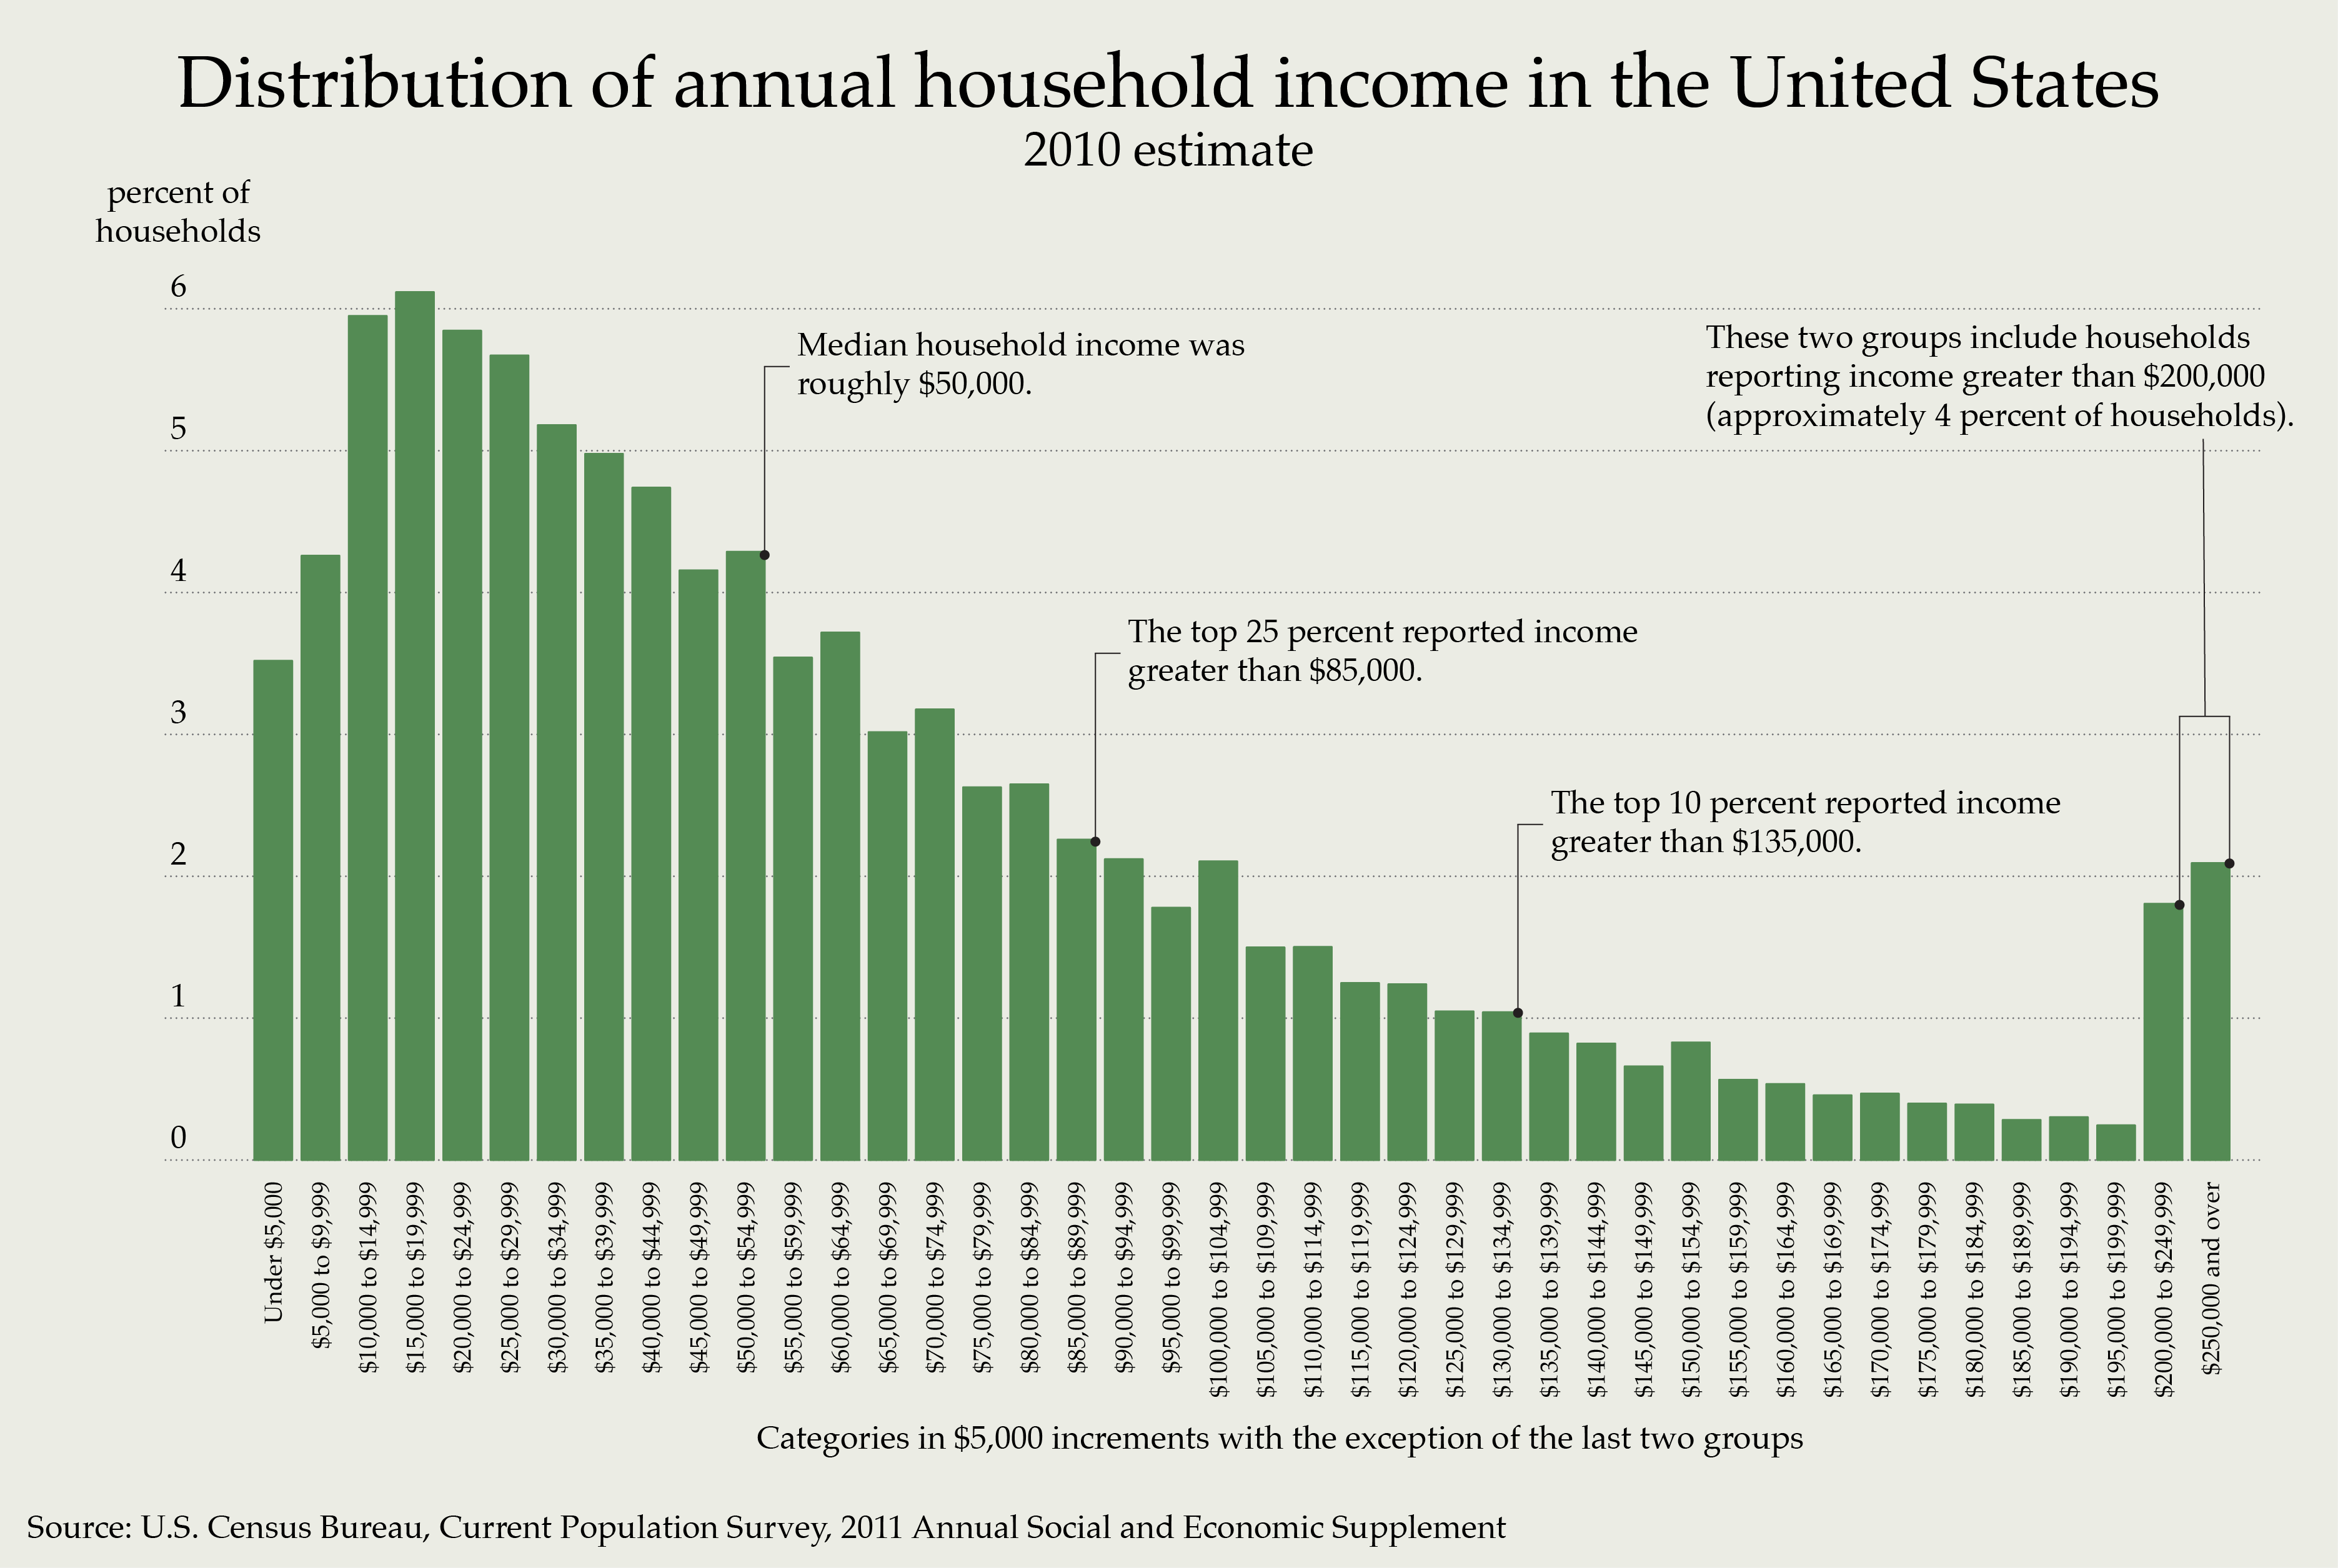
\includegraphics[width=\textwidth]{./figures/Distribution_of_Annual_Household_Income_in_the_United_States_2010.png}
    \caption{Example of a more natural weight distribution with a power law tail but not for smaller weights.}
    \label{fig:natural_weight_distribution}
\end{figure}

% This is particularly true as power laws 
% A sequence of weights with a constant q-tile of largest weights fitting into $\tau$ powerlaw tramlines fits the general GIRG formulation, but could still look quite different based on the distribution of the smaller weights.

An easy improvement to better fit a specific real graph is to take the sequence of node degrees as weights
\footnote{these are now all positive integers $\geq 1$ as opposed to real numbers $\geq x_{\min}$, since in the largest connected componenet, minimum degree is 1}. Copying degrees as weights makes sense due to the Chung-Lu like property of having $E[d_u] \propto w_u$, whose correct scaling can be made correct by fitting $c$ as detailed in the next section. 
% For the GIRG model however there is the added complication of node locations, whereby a node might have a higher degree than expected for its weight $w_u$, by fortune of having many geometrically close nearby nodes $\vec{x}_v$.
% This would clearly have better classification performance than power law generating weights.
For the classification comparison framework, Blasius actually uses weight copying for fitting the Chung-Lu GGM, but not for the hyperbolic GGM (which is odd). This doesn't make a fair / like for like comparison, so we cover all bases by having both weight copied and power law fit GIRGs, as well as adding in a power law fit Chung-Lu. ER and BA GGMs are still just fit on the courser metric of overall graph average degree, as they have little ability to replicate a power law degree distribution.

Comparing weight copied Chung-Lu with weight copied GIRGs was additionally interesting for harder feature sets where other GGMs struggled to get below 98\% classification accuracy - having such high constrained numbers makes it harder to compare meaningfully between GGMs (drawing conclusions from 98\% vs 99\% is tough)

% Comparing weight copied Chung-Lu with weight copied GIRGs was additionally interesting as their classification from real graphs was harder and hence more informative (trying to compare a 97\% vs 99\% classification accuracy is less meaningful than a 80\% vs 90\%).

% (QUESTION: does the GIRG formulation actually guarantee that as n -> infinity you couldn't tell the difference? I don't think so. E.g. if 1/4 of nodes had w=1, 1/4 had w=10 and 1/2 were power law above 10 distributed.)


\begin{comment}
Integrating $\int_w w^{-\tau} \PP(\Poisson(\Theta(w)) = x) dw$ gives $\E[dd(x)] = \Theta(x^{-\tau})$, for large $x$, dropping smaller order terms.


If instead, independently, each $d_u = \E[\Poisson(\Theta(w_u))] = \Theta(w_u)$, then we would sort of be able to say that the degree distribution follows a $\tau$ exponentiated power law distribution.
We would argue that independently, $P(d_u=m) \approxeq \Theta( \int_{m-1/2}^{m+1/2} w^{-\tau}) = \Theta(m^{-\tau})$, and hence that $dd(m) \sim \frac{Bin(n, m^{-\tau})}{n} \to N(m^{-\tau}, \frac{m^{-\tau}(1- m^{-\tau})}{n}) \approxeq m^{-\tau}$.

Ok so now if $d_u \sim \Poisson(\Theta(w_u))$, can we then derive $\PP(d_u = d)$? $\PP(d_u = d) = \int_W \PP(d_u = d | w_u = w) p(w) dw$. For large $w$, we approximate $\Poisson(\Theta(w_u)) \approxeq N(\Theta(w_u), \Theta(w_u))$. Hence we get $\PP(d_u = d) \propto \int_W \exp(-\frac{(w-d)^2}{2w}) w^{-\tau} dw$. We approximate this integral to be dominated by the interval $w \in [d - k\sqrt{d}, d + k\sqrt{d}]$ for sufficiently large $k$.

So we get $\PP(d_u = d) \propto \int_{d - k\sqrt{d}}^{d + k\sqrt{d}} \exp(-\frac{(w-d)^2}{2w}) w^{-\tau} dw \approxeq \int_{d - k\sqrt{d}}^{d + k\sqrt{d}} \exp(-\frac{(w-d)^2}{2d}) w^{-\tau} dw$. 

Substitute in $x = w - d$ to get $\int_{-k \sqrt{d}}^{k \sqrt{d}} (d + x)^{-\tau} e^{-x^2/2d}dx$.

Then using $(d + x)^{-\tau} = d^{-\tau} (1 + \frac{x}{d})^{-\tau} \approxeq d^{-\tau} (1 - \frac{\tau x}{d} + \frac{\tau(\tau+1)}{2} \frac{x^2}{d^2})$ for $x \in [-k \sqrt{d}, k \sqrt{d}]$, we get $\int_{-k \sqrt{d}}^{k \sqrt{d}} (d + x)^{-\tau} e^{-x^2/2d}dx \approxeq d^{-\tau} \int_{-k \sqrt{d}}^{k \sqrt{d}} (1 - \frac{\tau x}{d} + \frac{\tau(\tau+1)}{2} \frac{x^2}{d^2}) e^{-x^2/2d}dx$.

Finally we can use the results on the pdf of a normal distribution integrating to $1$; the mean integrating to $0$, and the variance integrating to $\sigma^2$, to get that $\PP(d_u = d) \propto d^{-\tau} (1 + \frac{\tau(\tau + 1)}{2} d^{-2} d) = d^{-\tau} 1 + \frac{\tau(\tau + 1)}{2} d^{-(\tau + 1)}$. This formula is essentially a weighted average between two different power law distributions. As $d \to \infty$ it will actually be correct, and be dominated by the larger $d^{-\tau}$ term. However for not so large $d$, it will be more a mix, and so the "perceived/empirical" powerlaw exponent could look larger, presumably somewhere in $[\tau, \tau + 1]$.


None of this is quite true as $d_u$ aren't independent: doubly so, 1. due to weights, and 2. due to positions. 

Hence for a GIRG, $ \E[dd(x)]  \propto x^{-\tau}$ for $x_\text{min} < x \in \N$, a lower cutoff point. This cutoff is necessary not just because the pdf would blow up at $x=0$, but also because the power law behaviour may only hold for higher degrees. The GIRG 
\end{comment}


\subsection{Fitting $c$ and $\alpha$}
\label{subsec:fitting_c_and_alpha}
These are our last two GIRG parameters to fit.
The parameter $c \in \R^+$ is most directly linked to the generated graph's average degree, whereas the parameter $\alpha \in (1, \infty]$ is more linked to the power of the geometry - larger $\alpha$ decreases the probability of longer distance edges which have $\rho_{uv} < 1$, leaving the edge set more dominated by shorter (and hence more geometric and clustered) edges. We therefore follow \cite{blasius2018towards} by fitting $\alpha$ with the clustering coefficient. Regrettably we used in our experiments the mean \textit{local clustering coefficient (LCC)} to fit our GIRGs and Hyperbolic Random Graphs, 
\begin{equation}
    \mathrm{LCC}(G) := \frac{1}{|V|} \sum_{u \in V} 
    \frac{| \{ v, v' \in \Gamma(u): v \sim v'\} |}{{|\Gamma(u)| \choose 2}} \in [0, 1]
\end{equation}
instead of the global clustering coefficient as in \cite{blasius2018towards}. $\Gamma(u)$ is the set of neighbours of $u$, so LCC counts the fraction of pairs of neighbours of $u$ that possess the triangle completing third edge. The global clustering coefficient is the fraction of total \q{V} shapes that indeed are completed as full triangles and is likely a better metric than the LCC. Luckily in practice they generally differ by less than 1\%.

Unfortunately $c$ and $\alpha$ are not wholly independent, so we must fit them in tandem, fitting $c$ for a given $\alpha$ so as to match the average degree of $G$, and then $\alpha$ for that given $c$ to match the LCC of $G$. This then looks like coordinate ascent in 2D: we alternatingly set $c \gets \hat{c}_1;\; \alpha \gets \hat{\alpha}_1;\; c \gets \hat{c}_2;\; \alpha \gets \hat{\alpha}_2;\; ...$.

Fitting $\alpha \gets \hat{\alpha}_i$ based on LCC is precisely ABC like - we propose potential $\alpha_i$ values, for which we generate a graph $G' \sim \cG_{\GIRG}(n, d, \hat{c}_i, \alpha_i, \tau)$, and use the distance metric $\delta(G, G') = |\mathrm{LCC}(G) - \mathrm{LCC}(G')|$ to both propose a next candidate $\alpha_i$ and eventually accept the final best $\hat{\alpha}_i$. Expected mean LCC is monotone in $\alpha$ so we know which direction to make a new proposal, and we follow \cite{blasius2018towards} in doing binary search in $\alpha^{-1}$ search space with starting bounds $[0. 1)$.

\cite{blasius2022efficiently} luckily gives a more efficient method to fit $c$ given $\alpha, d$, and a pre-sampled set of weights $(w_u)_{u \in V}$, that doesn't involve fully sampling a new $G' \sim \cG_{\GIRG}$. They derive a formula for the expected average degree $\E[\overline{deg}(G')]$ of the GIRG which looks, emphasizing the dependence on $c$, like:
\begin{equation}
    \label{eq:expected_edge_degree}
    \E[\overline{deg}(G') | c] = c A + c^{1/\alpha} B
\end{equation}
Hence we just have to numerically solve \cref{eq:expected_edge_degree} for $\hat{c}: \E[\overline{deg}(G') | \hat{c}] = \overline{deg}(G) = 2 |E|/|V|$ in order to obtain our desired average degree. Blasius provides C++ code for this, which finds $\hat{c}$ with a binary search.

The expected average degree formula of \cref{eq:expected_edge_degree} miraculously holds for all volume based toroidal GIRGs (regardless of exact disance function $r(x_u, x_v) = r_{uv}$), and we can even adapt the formula to be independent of dimension $d$.

\subsection{Volume formulation torus GIRG expected average degree formula}
\label{subsec:average_degree_formula}
% The volume formulation of a GIRG presented in \cite{bringmann2019geometric} provides a useful generalisation of the GIRG model:
% \begin{equation}
%     p_{uv}(r) = \min \left \{ 
%         1,
%         c \left (
%             \frac{w_u w_v / W}{Vol(r_{uv})}
%         \right )^\alpha    
%     \right \}; \quad \rho_{uv} = \frac{w_u w_v / W}{Vol(r_{uv})}
% \end{equation}
% Here $Vol(r_{uv}) = Vol(B_{r_{uv}})$ is the volume of the ball of radius $r$ using the distance function $r(x_u, x_v) = r_{uv}$, which must be symmetric to make sense.
% For example in the $\infty$-norm, $Vol(r_{uv}) = (2r_{uv})^d$ as a cube with side-length $2r_{uv}$.

% Having volume in the edge probability formula is actually a generalisation of taking $r_{uv}$ to the dth power - the point being to make $p(u \sim v | x_u, w_u, w_v) = E_r[p_{uv}(r)] = \Theta(w_u w_v/n)$, regardless of dimension.
In this subsection we calculate $E_r[p_{uv}(r) | c]$ in a volume formulated GIRG, whose volume function is denoted $Vol(r)$ (could correspond to any of max norm, euclidean norm, MCD etc.), and arbitrary dimension $d$ torus geometry $\chi = \T^d$.

Given a fixed weight sequence $(w_u)_{u \in V}$ we will recover \cref{eq:expected_edge_degree} via 
\begin{equation}
    E[\overline{deg}(G') | c] = \frac{1}{n} \sum_{u \in V} \sum_{v \in V} E_r[p_{uv}(r)]
\end{equation}
% We'll derive the same resultant $p(u \sim v | w_u, w_v) = \E_r[p_{uv}(r)]$ regardless, relying only on the fact that $Vol(r)$ is an increasing function. Finally, $\E[d_u] = \sum_v p(u \sim v | w_u, w_v)$ and hence $\E[\overline{deg}] = \sum_u \E[d_u]$.
Now $E_r[p_{uv}(r)] = \int_r p_{uv}(r) p(r) dr$. We'll break this down into $\int_{r: \rho_{uv} \geq 1} + \int_{r: \rho_{uv} < 1}$ (short edges and long edges, corresponding to edge probabilities being capped at 1, or strictly less than one for larger inter node distances) and write $\hat{r} : Vol(\hat{r}) = c^{1/\alpha} \left ( \frac{w_u w_v}{W} \right )$ as the boundary at which $\rho_{uv} = 1$.

Hence we get $E_r[p_{uv}(r)] = \int_0^{\hat{r}} p(r) dr + \int_{\hat{r}}^{r_{\max}} p_{uv}(r) p(r) dr$.

Substituting $Vol = Vol(r);\; dr = dVol \frac{dr}{dVol} = \frac{dVol}{p(r)}$, we get:
\begin{align}
    E_r[p_{uv}(r)] =& 
    \int_0^{Vol(\hat{r})} dVol + 
    \int_{Vol(\hat{r})}^{Vol(\mathbb{T})} p_{uv}(Vol) dVol
    \\
    =&
    Vol(\hat{r}) + 
    \int_{Vol(\hat{r})}^{Vol(\mathbb{T})} 
    c \left (\frac{w_u w_v}{W} \right )^\alpha Vol^{-\alpha}  
        dVol
    \\
    =&
    Vol(\hat{r}) + 
    c \left (\frac{w_u w_v}{W} \right )^\alpha \frac{1}{\alpha - 1}
        \left [
            \left (\frac{w_u w_v}{W} \right )^{1 - \alpha} c^{\frac{1 - \alpha}{\alpha}} - 1
        \right ]
    \\
    =&
    c^{1/\alpha} \left (\frac{w_u w_v}{W} \right ) 
        \left [ 1 + \frac{1}{\alpha - 1} \right ] 
    - 
    \frac{c}{\alpha - 1} \left (\frac{w_u w_v}{W} \right )^\alpha
    \label{eq:p_u_to_v_marginal_on_position}
\end{align}
where in the last two lines we sub in $Vol(\hat{r}) = c^{1/\alpha} \left (\frac{w_u w_v}{n} \right )$, and $Vol(\mathbb{T}) = 1$.
I.e. across all GIRGs of different distance functions and dimensions $d$, we get the same resultant edge probabilities when marginalising out node locations. Note this is also $\Theta(\frac{w_u w_v}{W})$ since $\alpha > 1$, which shows the similarity between GIRGs and Chung-Lu!

Following \cite{blasius2022efficiently} Appendix, the formula just needs a correction for pairs $u, v$ such that $Vol(\hat{r}) = c^{1/\alpha} \left ( \frac{w_u w_v}{n} \right ) > 1$, for which the second integral is unnecessary, and the first's upper bound is capped lower at $1$, the volume of the torus. These are (rare) pairs of nodes $u, v$ which have such giant weights $w_u, w_v$ that $p_{uv}(r) = 1$ identically, no matter how far apart $x_u, x_v$ are placed in the torus.



\subsection{Estimating const $c$ in Cube GIRGs}
To fit $c$ for a specific real graph $G$, for torus GIRGs we solved for the equation $f(c) = \overline{deg}$, given fixed $\alpha$. Our distance based Cube GIRGs have fewer edges in expectation than their toroidal counterparts, and no nice formula for the expected average degree. Instead we estimate $\hat{c}$ by starting with an initial guess $c_0=1$, and iteratively updating by each time generating a graph $G_i \sim \GIRG(c_i)$ and setting $c_{i+1} \gets c_i \frac{n \, \overline{deg}}{2 |E(G_i)|}$ until convergence.


\section{Realism Framework Results}
As introduced in \cref{sec:ggm_blasius_framework}, we fit a selection of GGMs, including various different kinds of GIRG on 104 socfb Facebook graphs, whose sizes range from $n=762$ to $n=35,111$ nodes. With each GGM we generated a mirrored dataset of fake graphs, with which we train a sequence of SVM classifiers to distinguish between the real and fake datasets, differing on which high level graph features they use as input. Classification accuracy using a particular GGM and feature set could be e.g. 100\% if the fake graphs are highly unrealistic in these features, or as good as 50\% if they're indistinguishable from the real graphs. Our results are shown in \cref{fig:blasius_framework_table} and \cref{fig:blasius_framework_means}, along with a \q{control} in \cref{fig:blasius_framework_means_1d_base} which classifies GGM fake datasets against the 1d max torus generated graphs instead of the real graphs. The numbers displayed in all three are actually the \textit{misclassifcation rate}, i.e. $1 - \text{accuracy}$, so that higher numbers mean more realistic GGM fit.

In \cref{fig:blasius_framework_table} we present results of the harder classification test of using a whole distribution of node-level features. E.g. one node level property \q{deg}  actually means the inclusion of 5 features describing the distribution of node degrees: mean, median, lower quartile, upper quartile and standard deviation. In contrast the classification results in \cref{fig:blasius_framework_means} and \cref{fig:blasius_framework_means_1d_base} just use the mean node level features, which makes it easier to fool the classifier. Having more significantly higher than zero misclassification rate numbers in \cref{fig:blasius_framework_means} allows for more  meaningful comparisons between different GGMs and across a wider range of features.
% Higher classification accuracies, e.g. $99\%$, denote that the GGM generates are readily distinguishable from the real graphs, and hence the GGM is a poor / unrealistic fit; $50\%$ accuracy is the gold standard of real/fake indistinguishability on the feature set.

% We can see from \cref{fig:blasius_framework_table} that mimicking the features of real Facebook graphs with generations from a fit GGM is tough. For example in the feature set (n, m, deg), by deg we mean to include 5 numbers per graph: mean node degree; lower, middle (median) and upper quartile node degree, and standard deviation over all node degrees. Our numbers can be compared to Table 2 in \cite{blasius2018towards}, which also includes feature sets with just mean node values, which in some cases makes fooling the classifier much easier\footnote{We do get similar results to Table 2 when training SVMs with just the mean node features, which can yield lower accuracies in the $50-70\%$ range}.

% seem low in places compared to \cite{blasius2018towards}, which is because we have a higher bar due to a more extensive feature set. For exmaple in the feature set (n, m, deg), by deg we include 5 numbers per graph: mean node degree; lower, middle (median) and upper quartile node degree, and standard deviation over all node degrees; \cite{blasius2018towards}'s Table 2 uses just mean value for node level features \footnote{We do get similar results to Table 2 when training SVMs with just the mean node features, which can yield lower accuracies in the $50-70\%$ range}. Features like k-cores and comms aren't node level, and are taken over the actual core/community sizes - so are e.g. mean, median etc. community sizes within a graph.

\paragraph{Types of GIRG tested in classification framework}
\begin{itemize}
    \item The \q{base} GIRG type is max norm torus GIRGs of dimension $d=1,2,...,7$
    \item MCD torus GIRGs for $d=2,3,4,5$ ($d=1$ is equivalent to max norm)
    \item Min/max mixed torus GIRGs with groupings 1-23; 1-234; 12-34; 1-2-34. E.g. 1-23 denotes $\norm{\vec{x} - \vec{y}} = \min \left \{ |x_1 - y_1|_C,\; \max(|x_2 - y_2|_C,\, |x_3 - y_3|_C) \right \}$
    \item Max norm cube GIRGs. We were held back due to the increased computation when fitting the average degree with constant $c$, so only include  $d=1,2,3$ cube GIRGs, and $d=1,2,3,4,5$ copy-weight cube GIRGs (an attempt for maximal realism)
    \item The host of simpler models CL (with power law fit weights, and with degree copied weights), BA, ER as in \cite{blasius2018towards}, as well as Hyperbolic random graphs which are very similar to 1d torus GIRGs
\end{itemize}

\paragraph{New classification features}
We additionally added features that were not assessed in \cite{blasius2018towards}. Shown in \cref{fig:blasius_framework_table} are the non-node-level features \q{k-cores, comms}. These denote k-core sizes and community sizes (communities found using the Louvain method).
However these can be rather high variance numbers. For example a 3000 node 2d max torus GIRG with average degree of 60 can end up with 40 k-cores and just 8 communities. This means that the community size distribution features would be the average size of these 8 communities, as well as lower, middle and upper quartile size and standard deviation of these sizes.

Unfortunately, for community sizes, even Erdos-Renyi graphs have a misclassification rate comparable to the other GGMs, so this feature seems useless.

% \subsection{Analysis of Classification Results}
% The framework of \cite{blasius2018towards} has its limitations, but we can draw some general conclusions.


\subsection{Degree distribution features}
% \subsubsection{Degree distribution features}
% \addtocounter{subsubsection}{1}
As noted in \cite{blasius2018towards} features like Katz centrality, PageRank, k-core number / k-core sizes, node degrees and node degree power law are more closely related to the degree distribution. Consequently they are less useful for distinguishing between different types of GIRG geometries.

For this group of features we naturally observe much better performance for copy-weight GIRGs / copy-weight Chung-Lu which have the most similar degree distributions to the real graphs - Chung-Lu doing the best as it has the purest degree alignment. For all these features  except \q{n, m, Katz} in \cref{fig:blasius_framework_table} (distribution features), non copy-weight GGMs have all zero misclassification rates. For k-core, deg and Katz, the copy-weight GIRGs also feature monotonically increasing misclassification rates with increasing dimension, presumably as higher dimensions make the GIRG more similar to the Chung-Lu - see \cite{friedrich2023cliques}.

For just mean features in \cref{fig:blasius_framework_means}, there are many more non-zero rates for non-copy-weight GGMs, but generally worse numbers than the copy-weight GGMs. For whatever reason, non-copy-weight 3d cube GIRGs are much better on k-core ($16\%$) than all other GGMs, even copy-weight 3d cube GIRGs which get just $7\%$, and decently better on Katz centrality ($17\%$) than the other non-copy-weight GGMs.
This could be due to a more realism of extreme nodes near the edge of the cube that both have a lowered degree, and neighbours which are also similarly low degree due to being extremely located.
% The copy weight GGMs do get up to $47\%$ on Katz, however oddly copy weight cube GIRGs have just $7-9\%$ misclassification rate on k-core.

\subsection{Geometric Features}
% \subsubsection{Geometric features}
% \addtocounter{subsubsection}{1}
The features betweenness centrality, closeness centrality, local clustering coefficient, diameter and effective diameter are more related to the geometry. GIRGs show on these features increased realism in comparison to the non geometric GGMs, and we can also compare between the different GIRG types: max / MCD / mixed distance functions; torus / cube geometries. We focus exclusively on the non-copy-weight GIRGs, with numbers from the mean based classifiers in \cref{fig:blasius_framework_means} rather than the distribution based classifiers in \cref{fig:blasius_framework_table} which have too low numbers for a good comparison. In the former, the copy-weight cube GIRGs have similar performance on these features - their more realistic degree distribution only help in the latter, more challenging simulation task.


Chung-Lu graphs are a good comparison point against GIRGs by being a similarly degree inhomogenous graph, just without any geometric influence.
\footnote{Another potential GGM geometry null hypothesis would have been the configuration model which tries to mimick a degree sequence, like Chung-Lu, but more strictly. Each node is given a set number of \q{half edges} which gives it a set degree (the degree sequence can be random e.g. power law generated, or given e.g. copied directly from a real graph). Half edges are then joined together at random.}.



Among non-copy-weight GIRGs, 1d max torus GIRGs are surprisingly best or close to best on many feature sets. This is evidence that the geometric component of real graphs is strongest in just one dimension, which we also see in \cref{chap:likelihood_point_estimation}. It would be interesting to see if 2d or 3d distorted GIRGs could do better on these features, as they would precisely exhibit geometry with one dominating dimension, and a few auxiliary ones.
On betweenness, 1d max torus GIRGs perform the best, with a slight decay for 2d-4d. Mixed GIRGs hold up well, but MCD GIRGs do much worse; cube GIRGs are only a little worse.
However MCD and mixed GIRGs do better on closeness than max GIRGs, especially 1-23 mixed GIRGs. This is actually evidence for the \q{one strong dimension} hypothesis, as 1-23 mixed GIRGs give more significance to their dim 1 over dims 2,3. We can even observe in \cref{fig:blasius_framework_means_1d_base} that 1-234 mixed GIRGs have such a strong force of their first dimension that they are hard to classify apart from 1d max torus GIRGs!

\paragraph{Effective diameter and cube GIRGs}
Cube GIRGs generally underperform, except on effective diameter, where they shine through as the best, with ranking 1cu\textless 2cu\textless 3cu. This makes sense as cube geometry doesn't impact many shortest paths, but rather does so on the longest shortest paths, between nodes at opposite extremes of the cube which would otherwise be shortcutted by the torus. We can dive into the data to see that our intuition seems correct: real effective diameters of FB graphs range from $3.0$ to $4.4$; 2d torus GIRGs' are too small, on average $0.17$ less than their real counterparts, while 2d cube GIRGs' are larger and on average just $0.04$ less.



% \paragraph{GIRGs performance}

% Copy-weight cube GIRGs have a clear cut performance advantage over all other GGMs, only rivalled by copy-weight Chung-Lu. We see, as expected, improvements in diameter and effective diameter over Chung-Lu, and just in effective diameter for non copy-weight GIRGs. Copy-weight GIRGs also have improved LCC performance over copy-weight Chung-Lu, though this is not observed in powerlaw weighted GIRGs - despite explicitly fitting the mean LCC, the wider LCC statistics must be quite distinguishable. 

% Not-surprisingly copy-weight GGMs have very good degree distribution performance, with Chung-Lu being the best as having no extra geometric modification on the copied degree sequence.

% Community sizes and k-core sizes are potentially less consistent features to consider as they have higher variance than node level features.


\paragraph{Local Clustering Coefficient (LCC)} Due to their geometry, GIRGs exhibit significant clustering just like real graphs. We explicitly match for the mean LCC in our GIRG fitting procedure, so it's not surprising that the \q{n, m, LCC} row in \cref{fig:blasius_framework_means} has near-perfect performance for most GIRGs, whereas all other GGMs have a $0\%$ misclassification rate as they have tiny mean LCCs. This drops to $0\%$ for all GIRGs except copy-weight cube GIRGs when classifying based on LCC distribution. \cite{blasius2018towards} explained this by showing their fit hyperbolic graphs to have too low variance, which is likely the case for GIRGs here too.

For mean LCC only 4d, 5d MCD GIRGs and 6d, 7d max GIRGs exhibit low misclassification rates, due to their inability to match the real graphs' high mean LCC. E.g. on socfb-Caltech36, the real graph has a mean LCC of $0.41$, however capping at $\alpha=100.0$ ($\alpha=\infty$ wouldn't improve the situation much either), the max norm 4d torus GIRG can only reach $0.33$, and the 5d GIRG just $0.24$. LCC is guaranteed to be non-tiny in GIRGs due to the triangle inequality: if $u \sim v_1$ and $u \sim v_2$ then likely $r(u, v_1), r(u, v_2)$ are both small, which makes $r(v_1, v_2) \leq r(u_, v_1) + r(u, v_2)$ also small. However for higher dimension GIRGs, $r(v_1, v_2)$ is more likely to be closer to this upper bound. LCC decays already for 4d MCD GIRGs as the MCD distance function isn't actually a metric so only obeys the triangle inequality stochastically (some percentage of the time. E.g. if $u$ is close to $v_1$ in dimension 1, and close to $v_2$ in dimension 2 then $v_1, v_2$ are generally not close to each other).


\begin{figure}
    \centering
    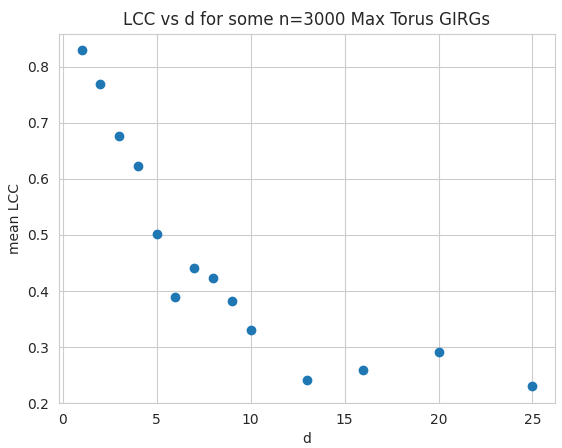
\includegraphics[width=0.8\textwidth]{./figures/LCC_vs_d.png}
    \caption{Increasing the dimension $d$ of a GIRG will decrease the mean LCC, but only up to a $\Theta(1)$ threshold due to the triangle inequality. Each point is one generated GIRG, all other parameters remaining fixed.}
    \label{fig:LCC_vs_d}
\end{figure}



% The first column of copy-weight cube GIRGs in \cref{fig:blasius_framework_table} have much better classification accuracy than the rest, apart from copy-weight Chung-Lu, which serves as the non-geometric comparison point. It would also be interesting to these GIRGs with the configuration model \footnote{Each node is given a set number of "half edges" which gives it a set degree (the degree sequence can be random e.g. power law generated, or given e.g. copied directly from a real graph. Half edges are then joined together at random.)} with copied degrees as the "null hypothesis" against these.

% In notably geometric feature categories like LCC, and diameter GIRGs indeed out perform Chung-Lu.
% Chung-Lu does better on community size statistics; communities could arguably spring from geometry, but GIRGs' uniformly random geometry isn't really designed for this - you could rather imagine a more realistic setup if node locations were taken from a mixture of gaussian distributions (e.g. a university town might have age/occupation clusters of student age vs working age, or academic vs non-academic peoples).


\subsection{Case study of distribution vs mean based classification: closeness centrality}
% \subsubsection{Case study of distribution vs mean accuracy: closeness centrality}
% \addtocounter{subsubsection}{1}
In \cref{fig:blasius_framework_table} which provides feature distributions as input to the SVM classifier, it is disappointing that non copy-weight GIRGs show such poor performance, even on \q{geometric} features like closeness, betweenness and LCC (at least on closeness and betweenness they still recognizably outperform CL, BA and ER). E.g. 2d max torus GIRGs have a misclassification rate of just $1\%$ on \q{n, m, betw} and $2\%$ on \q{n, m, close}, compared to much better $38\%$ and $28\%$ on the mean based classifier equivalents. To explain this large disparity we do a case study on closeness, which happily also assuages some of our concerns.

\cref{fig:real_2d_closeness_mean_scatter} shows that mean closeness aligns very accurately to the real graphs. Nonetheless, due to a consistently lower standard deviation of closeness in the GIRGs and the fact that the standard deviation of closeness in real graphs fits well as a function of number of nodes, the 2d GIRGs are distinguishable from real graphs on this feature set. We hence find the $2\%$ misclassification rate misleadingly low, and the GIRG's realism in closeness somewhat vindicated.

% This analsyis is similar to that done in \cite{blasius2018towards} to explain $0\%$ LCC misclassification rates for hyperbolic graphs when taking into account distribution of features - they found that hyperbolic graphs have consistently too low LCC standard deviation.

\begin{figure}
    \centering
    \begin{subfigure}{0.45\textwidth}
    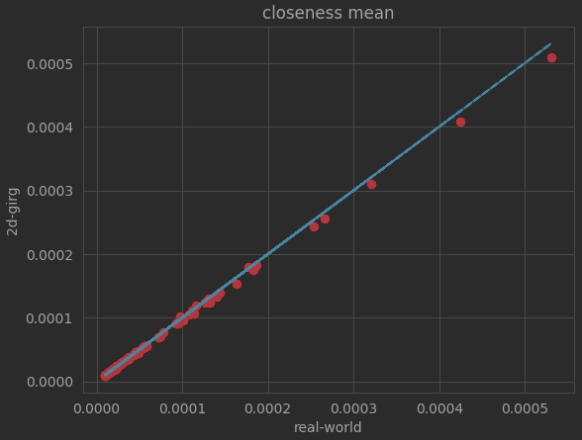
\includegraphics[width=\linewidth]{./figures/real_2d_closeness_mean_scatter.png}
    \caption{2d GIRGs have almost identical mean node closeness to real-world FB graphs; $y=x$ line shown in blue.}
    \label{fig:real_2d_closeness_mean_scatter}
    \end{subfigure}
    \begin{subfigure}{0.45\textwidth}
    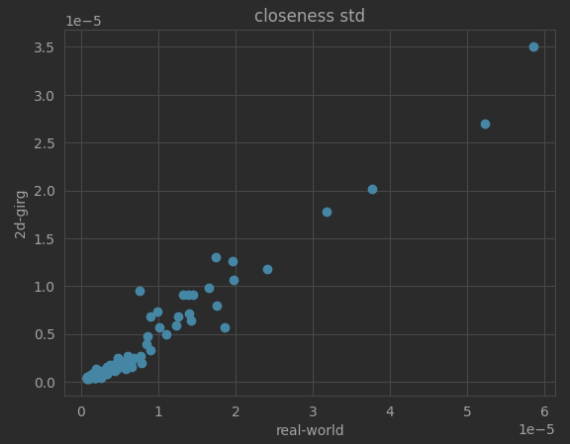
\includegraphics[width= \linewidth]{./figures/real_2d_closeness_std_scatter.png}
    \caption{2d GIRGs have consistently lower standard deviation of node closeness than real-world FB graphs}
    \end{subfigure}

    \parbox[b]{.5\textwidth}{\Large
    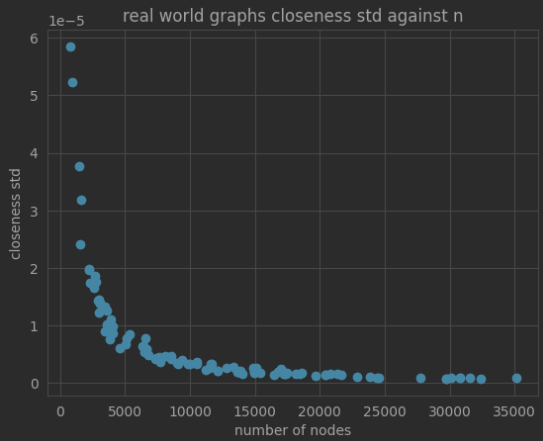
\includegraphics[width=0.9\linewidth]{./figures/real_closeness_std_against_n.png}
    \subcaption{Standard deviation of node closeness in real-world FB graphs fits well as a function of number of nodes}
    }
    \hspace{.05\textwidth}%
    \parbox[b]{.4\textwidth}{%
    \caption{Closeness centrality case study on fit 2d max torus GIRGs against their real counterparts. In plots (a) and (b), each dot is a real / fake graph pair, with the x/y value being the specifid feature's vale for the real/fake graph respectively. In plot (c), each dot is a real graph.}}
    % \begin{subfigure}{0.4\textwidth}
    % 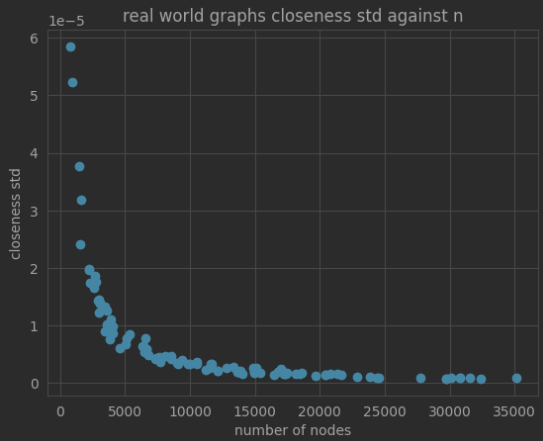
\includegraphics[width=\linewidth]{./figures/real_closeness_std_against_n.png}
    % \caption{standrd deviation of node closeness in real-world FB graphs fits well as a function of number of nodes}
    % \end{subfigure}
    % \caption{Closeness centrality case study on fit 2d max torus GIRGs against their real counterparts. In plots (a) and (b), each dot is a real / fake graph pair, with the x/y value being the specifid feature's vale for the real/fake graph respectively. In plot (c), each dot is a real graph.}
\end{figure}

\subsection{One drawback to the classification realism framework}
Classification accuracy is regrettably a crude metric. One limitation of this framework is that the attainable accuracy is also affected by the level of variance of a feature set across the real graph dataset relative to the fake dataset. GGMs generally end up with their features concentrated in a small subsection of the feature space, so if the real graphs are more spread out, it may be easier to overlap with a portion of their feature data points and attain a low but appreciable misclassification rate. However if the real graphs are less spread out they can miss altogether and get a minuscule misclassifcation rate. See \cref{fig:low_var_high_var_svm_clumps} for an illustration of different scenarios. In this case of closeness, the real graph feature vectors fit quite a precise pattern and hence the GIRG feature vector clump, though just slightly off, has little overlap.


\begin{figure}
    \centering
    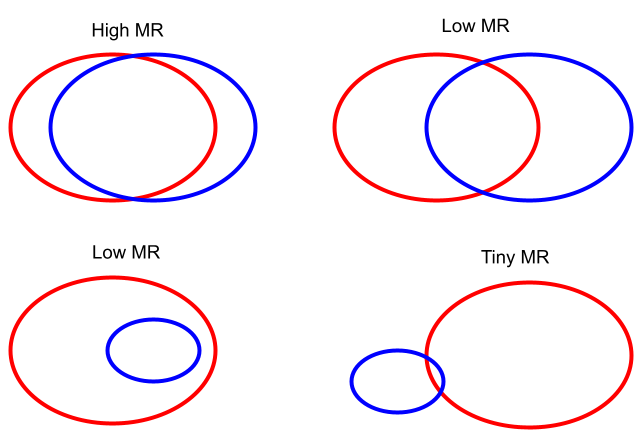
\includegraphics[width=0.9\textwidth]{./figures/VennDiagram.png}
    \caption{Illustration of SVM misclassification rates (MR) given different positions and variance of binary clusters. Red and blue ovals represent roughly gaussian distributed clusters of real and fake data points in a 2 dimensional feature space. An SVM would divide the space so as to maximise classification accuracy. How high accuracy it achieves is directly related to the area/density of overlap between the two clusters.}
    \label{fig:low_var_high_var_svm_clumps}
\end{figure}

% \begin{figure}
%     \centering
%     \begin{subfigure}{0.7\textwidth}
%         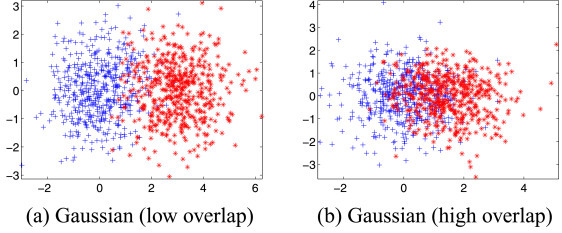
\includegraphics[width=\linewidth]{./figures/high_var_clump_overlaps.png}
%     \end{subfigure}
%     \begin{subfigure}{0.7\textwidth}
%     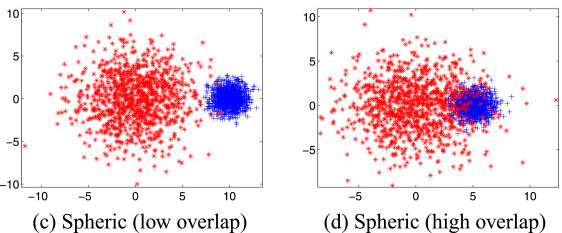
\includegraphics[width=\linewidth]{./figures/low_var_clump_overlaps.png}
%     \end{subfigure}
%     \caption{Plot taken from \cite{kefi2019novel} ("A novel incremental one-class support vector machine based on low variance direction")}
%     \label{fig:low_var_high_var_svm_clumps}
% \end{figure}

% (cube GIRGs having slightly larger diameters - to get from one edge of the cube to the opposite), but does fit our geometric intuition.


% does slightly fit our intuition of their more realistic geometry. Funnily enough Cube GIRGs fit on the dataset have 

% just mean that toroidal GIRGs have too large diameters compared to real graph (cube GIRGs having smaller diameters), but does fit our geometric intuition.

% 2+d min girgs we expect to have very large diameters.

\subsection{SVM Classifier Misclassification Rates Tables}

\begin{sidewaysfigure}
    \centering
    % \begin{subfigure}
    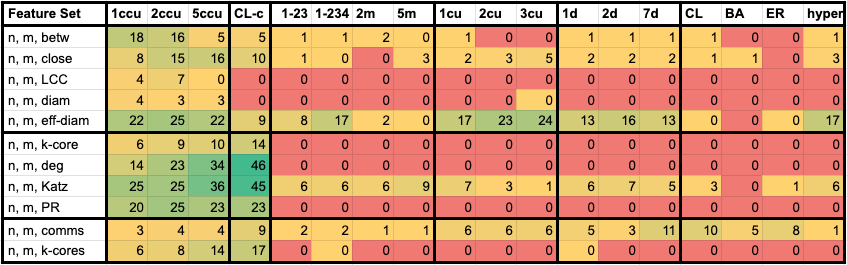
\includegraphics[width=\textwidth]{./figures/Blasius_framework_table.png}
    \caption{\cite{blasius2018towards} GGM realism framework results on Facebook graphs, extended to different GIRG models. Shown here are distribution based features, i.e. including mean, median, lower quartile, upper quartile and standard deviation of node level features.
    % If just one of mean/median is used, accuracies are often lower, sometimes even in $50\%-70\%$. $50\%$ is the best possible validation of a GGM as indistinguishable from real data, and is only achieved for feature set $n, m, LCC \;\text{mean}$ (by GIRGs and not the other none geometric GGMs).
    Some models are missing from the table e.g. 3d-6d GIRGs as their results follow a trend from low to high dimension.
    }
    \label{fig:blasius_framework_table}
    % \end{subfigure}
    \vspace{1em}
    \centering
    % \begin{subfigure}
    \begin{tabular}{|c|c||c|c|}
        \hline
        1-ccu & 1d copy-weight cube GIRG 
        & betw & betweenness centrality
        \\
        1-23 & $1 \lor (2 \land 3)$ mixed min/max GIRG
        & k-core & node k-core number
        \\
        2-min & $1 \lor 2$ 2d min GIRG
        & close & closeness centrality
        \\
        3-cu & 3d cube GIRG
        & LCC & node local clustering coefficient
        \\
        7d & 7d GIRG
        & deg & node degree
        \\
        CL & Chung-Lu
        & Katz & node Katz centrality
        \\
        CL-c & copy-weight Chung-Lu
        & PR & node PageRank
        \\
        BA & Barabasi-Albert
        & comms & community sizes
        \\
        ER & Erdos-Renyi
        & k-cores & k-core sizes
        \\
        hyper & Hyperbolic Random Graph &
        diam & graph diameter
        \\
        && eff-diam & graph effective diameter\\
        \hline
    \end{tabular}
    \caption{Graph Generative Model abbreviations; feature name abbreviations. Used in our results tables}
% \end{subfigure}
\end{sidewaysfigure}

\begin{sidewaysfigure}
    \centering
    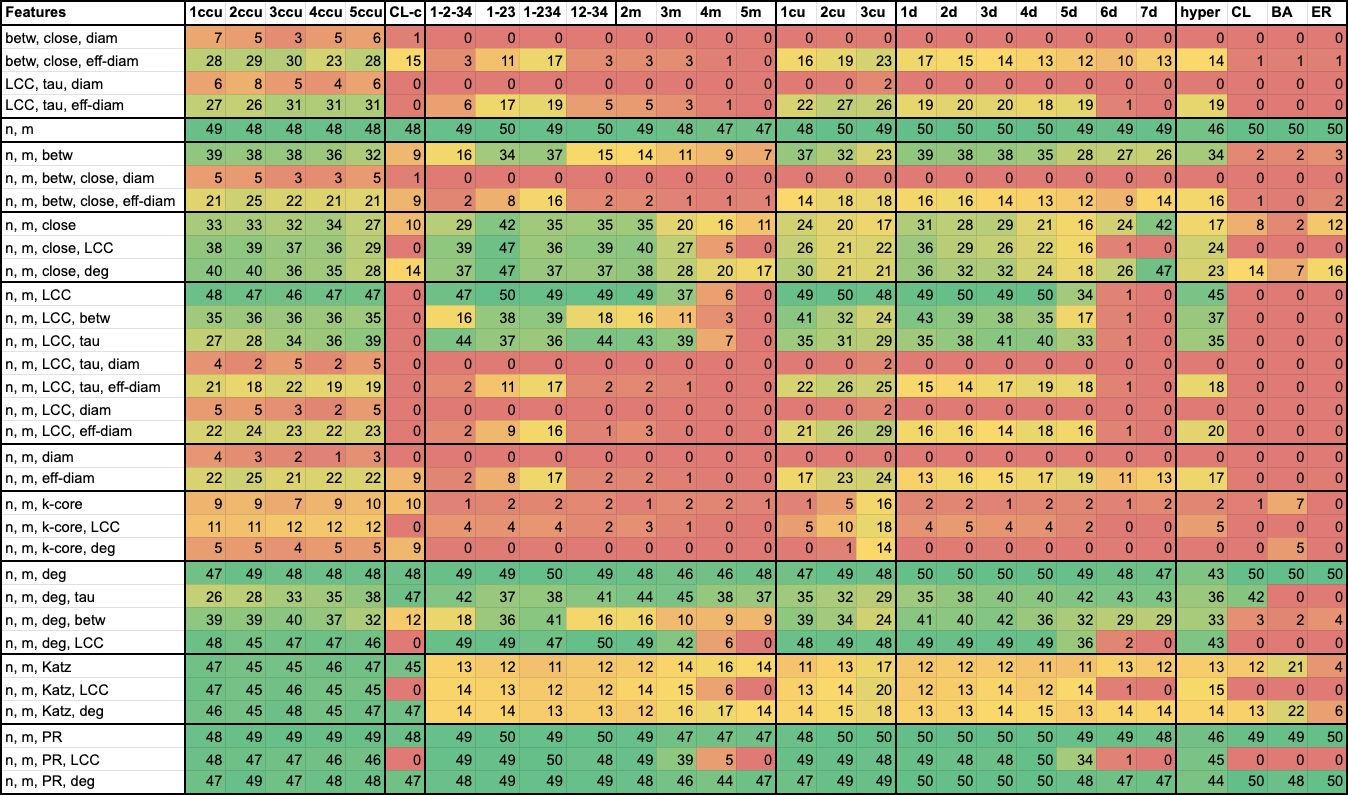
\includegraphics[width=\textwidth]{./figures/blasius_framework_means.png}
    \caption{Blasius Framework classification results based on just mean feature values}
    \label{fig:blasius_framework_means}
\end{sidewaysfigure}


\begin{sidewaysfigure}
    \centering
    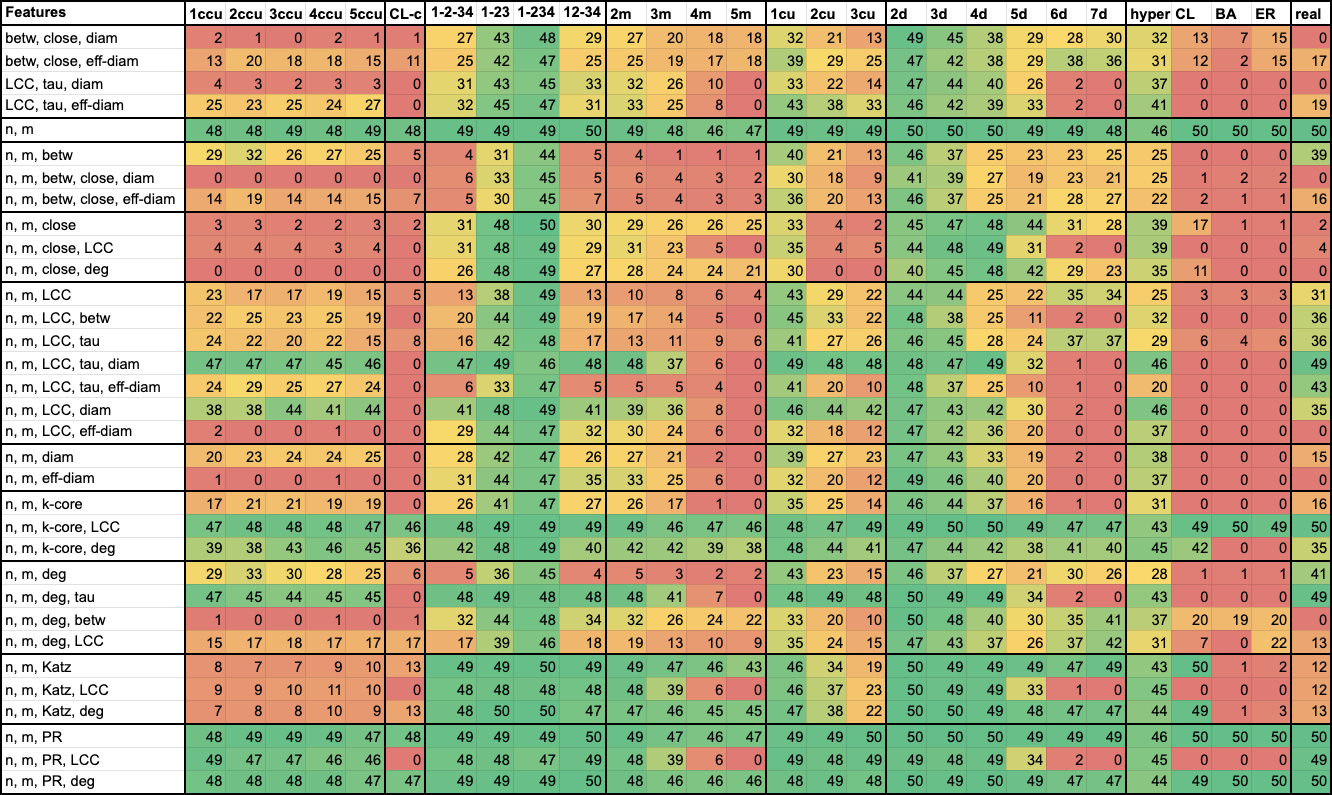
\includegraphics[width=\textwidth]{./figures/blasius_framework_means_1d_base.png}
    \caption{Blasius Framework classification results based on just mean feature values - \q{control} here by classification against the 1d max norm torus GIRG. I.e. all GGMs are still fit to the real graph (so for GIRGs mostly having matching mean node degre and mean LCC), but now the SVM is classifying each GGM against the 1d max norm torus GIRG instead of the real graph.}
    \label{fig:blasius_framework_means_1d_base}
\end{sidewaysfigure}
\chapter{Introduction}
\label{chap:introduction}
% \minitoc
\section{Thesis Introduction}
Graphs are a useful model for describing networks of interconnected entities as an abstraction of real-life systems. Real-world graph data are abundant, and many graphs exhibit similar structural characteristics. Several graph-generating models have been proposed, each justified by its reasonable formative mechanisms which create sets of graphs similar to those observed in the wild. Studying these generative models theoretically provides insights into real networks and is useful for creating synthetic graphs for testing purposes.

\textit{Geometric Inhomogeneous Random Graphs (GIRGs)} are one such graph-generating model, first proposed in \cite{bringmann2016average} as a generalisation of \textit{Hyperbolic Random Graphs}. GIRGs allow significant flexibility in the geometric component of their generative structure, thereby enabling better modeling of a broader range of real graphs. Their definition encapsulates the intuitive notion present in many graphs that nodes are more likely to be connected if they are \q{close together}. Furthermore, GIRGs exhibit inhomogeneity between nodes, resulting in a power law degree distribution, a characteristic observed in many real graphs.

This thesis evaluates the ability of GIRGs to simulate a dataset of $104$ social network graphs obtained from the \href{https://networkrepository.com/}{Network Repository} (\cite{rossi2015network}, \url{https://networkrepository.com/}). These graphs represent Facebook social networks from various towns in the US, thus exhibiting structural similarities, and range from $n=1000$ to $n=100,000$ nodes. In \cref{chap:GGM}, we assess the mostly unmodified GIRG prior distribution of graphs based on their high-level similarities to the real graphs. In \cref{chap:likelihood_point_estimation}, we perform a more intensive posterior style fit of GIRG to replicate real graphs at the node/edge level.

In \cref{chap:GGM}, the first task of assessing GIRG prior realism is conducted using a high-level feature dataset classification comparison framework proposed in \cite{blasius2018towards}. Our results provide evidence that GIRGs are more realistic candidates than simpler generative models with respect to geometric features such as node closeness centrality, betweenness centrality, local clustering coefficient, and graph effective diameter.
We compare the realism of different GIRG variants on these features and find that while max norm torus GIRGs provide a good baseline, cube GIRGs perform better on graph effective diameter, and mixed/minimum component distance GIRGs excel in closeness centrality.
In most (but not all) cases, we find that a small geometric dimensionality of $d=1$ already provides near-peak GIRG realism, with little benefit from higher-dimensional GIRGs.

Additionally, in \cref{chap:graph_kernels}, we attempt to apply the method of \textit{graph kernels} as an alternative framework for model selection between the GIRG prior model and other generative graph models with respect to our real graph dataset. Unfortunately, we were unable to produce reasonable results.

% and with respect to which statistics that GIRGs are most realistic. Only on some statistics do additional geometric dimensions and varying the type of GIRG make much difference - most results don't differ much from the basic 1-dimensional GIRG.

% We additionally explore the use of Graph Kernels as an alternative framework to explicit sets of high level graph statistics, but fail to produce reasonable results.

In the second task of GIRG posterior fitting, we aim to infer the node geometric locations of a given posited GIRG generative model for an input real graph. In \cref{chap:diff_maps}, we explore the method of diffusion maps as a computationally fast initial estimate of locations with good internode distances, and as a means of proposing the underlying geometric dimensionality. In \cref{chap:likelihood_point_estimation}, we describe methods to further refine node locations using either a markov chain Monte Carlo or maximum likelihood-based fitting approach. The full fitting procedure exhibits decent performance in replicating real graphs and supports the hypothesis that one dimension is mostly sufficient for this dataset of social networks.

To support all objectives, we also cover the different types of GIRGs and their unique , and demonstrate practical methods for sampling and working with them.



\chapter{GIRGs - Variants and Generation}
\minitoc
\section{GIRGs definition}
\label{sec:GIRG_def}
In this section, we define GIRGs and identify their key features.

As per \cite{bringmann2019geometric}, the GIRG model is a random graph model characterized by the edge connection probabilities given by the formula:

% TODO below (div by n, infty norm) is what I had before, but in fact bringmann2019geometric uses below with div by W and ambiguous norm.
% \begin{equation}
%     p_{uv} = \Theta \left ( \min \left \{
%         1,
%         c \left (
%             \frac{w_u w_v / n}{ \norm{x_u - x_v}_\infty^d}
%         \right )^\alpha
%     \right \}
%     \right )
% \end{equation}

\begin{equation}
    p_{uv} = \Theta \left ( \min \left \{
        1,
        \left (
            \frac{w_u w_v / W}{\norm{x_u - x_v}^d}
        \right )^\alpha
    \right \}
    \right )
\end{equation}

Here, $(w_u)_{u \in V}$ are node-specific weights in $\R^+$, and $(x_u \in \chi)_{u \in V}$ denote positions of nodes in a particular geometric space $\chi$, often taken to be the d-dimensional torus
\footnote{The d-dimensional torus also resembles $[0, 1]^d$, but opposite faces of the cube are identified. Picture Pac-Man, or donuts. Just not Pac-Man eating a donut...}
$\T^n$, or the d-dimensional unit cube $[0, 1]^d$.
The normalising factor $W^{-1}$, where $W = \sum_{u \in V} w_u$, ensures that the expected degree of a node $u$ remains constant even as $n \to \infty$; although $u$ will have more possible other nodes to connect with, this increase is counterbalanced by the declining probability of connecting to any one of them.


% This edge probability has a geometric factor from the distance $r_{uv} = \norm{x_u - x_v}_\infty$, which is taken to the dth power so that the number of edges is consistent across different values of $d$.
% This inversely scales the probabilities so that nearby points (small $r_{uv}$) are more likely to have an edge than those further apart.
% The $W^{-1}$ normalising factor ensures that for a node $u$, as $n$ increases (even $n \to \infty$), though it will have more possible other nodes to connect to, its expected degree won't change.

% Writing $\rho_{uv} = \left ( \frac{w_u w_v / W}{\norm{x_u - x_v}^d} \right )$ to save on writing, this is like the fundamental "score" of edge probability, which must be modulated to become the final probability (e.g. making sure its bounded above by 1).
% In particular the exponent $\alpha \in (1, \infty]$


\subsection{Geometry}
The geometric space $\chi$, along with the distance function written $r(\vec{x}_u, \vec{x}_v) = \norm{x_u - x_v} = r_{uv}$ (which is not necessarily a norm, or even a metric), can vary a great deal without affecting key properties of GIRGs.

The edge probability $p_{uv}$ incorporates a geometric factor from the distance $r_{uv}$, which inversely scales the probabilities so that nearby points (small $r_{uv}$) are more likely to have an edge than those further apart.
$r_{uv}$ is raised to the dth power to ensure consistency in the number of edges across different values of $d$.
This influence in GIRGs of node proximity on $p_{uv}$ facilitates the emergence of \textit{clustering}, a common phenomenon in many real-world graphs, where subgroups of nodes might have more internal edges than would be expected by chance.



% The geometric space $\chi$, and the distance function $\norm{\cdot}$ (not necessarily a norm) can vary a great deal without affecting the key properties of GIRGs. $\chi = \T^d$ the d-dim torus is very handy for proofs, as the viewpoint of any node $x_u$ is equivalently at the "centre" of the space. For real applications the d-dim cube $\chi = [0, 1]^d$ can be more realistic; however it is no longer symmetric; nodes with locations near the edge of the cube are different from those near the centre.

Using the \textit{max norm} as the distance function, i.e., $\norm{\vec{x}} = \norm{\vec{x}}_\infty = \max_i |x_i|$, is convenient for proofs, but can be replaced by euclidean or other norms - the equivalence of norms there is not much difference. Note that on the torus, the max norm is not strictly a norm, rather we abuse notation to express:
\begin{align}
    ||\vec{x} - \vec{y}||_\infty &= \max_i |x_i - y_i|_C\\
    |x_i - y_i|_C :&= \min(|x_i - y_i|, 1 - |x_i - y_i|)
\end{align}
The \textit{minimum component distance} (MCD), defined as $\norm{x}_{\mathrm{mcd}} = \min_i |x_i|$, does not even satisfy the triangle inequality, yet it preserves most properties of GIRGs. This distance function is reasonable if we desire two nodes to have a higher edge probability if they are close in at least one dimension, rather than in every dimension.

$\alpha \in (1, \infty]$ is a parameter that impacts the affect of geometry on edge probabilites. We differentiate between \textit{short edges} where $r_{uv} < (w_u w_v / W)^{1/d}$ and $p_{uv} = \Theta(1)$ (for these, the $\min(\cdot, 1)$ is applied to ensure $p_{uv} \leq 1$), and \textit{long edges}, where $r_{uv} > (w_u w_v / W)^{1/d}$, and $p_{uv}$ diminishes to zero as the distance increases. Larger values of $\alpha$ accelerate this decay in long edge probability, thus more severely limiting the number of long-distance edges. $\alpha=\infty$ imposes a strict cutoff, setting $p_{uv} = 0$ for long edges.

% The reason for the power of $d$ in $r_{uv}^d$ is to keep the edge probabilties equivalent with respect to the volume of space in different dimensions.
% The more general formula replaces replaces $||x_u - x_v||^d = r_{uv}^d$ with $Vol(B_r)$ the volume of the ball of radius $r=r_{uv}$.
% For norms, $Vol(B_r) = \Theta(r^d)$, e.g. in the $\infty$-norm, $Vol(B_r) = (2r)^d$ as a cube with side-length $2r$.
% The euclidean ball has some $\pi$'s in the formula. For the minimum component distance, $Vol(B_r) = \Theta(r)$.
% Volumetric equivalence makes sense in that the edge probability $p_{uv} | x_u, w_u, w_v$ in the Torus is determined by integrating $\int_{r=0}^{r=1} p_{uv}(r) p(r) dr = \int_{Vol=0}^{Vol=1} p_{uv}(Vol) dVol$, where $Vol(r) = Vol(B_r)$ is the volume of the ball of radius $r$.
% Hence across different GIRGs of different dimensions $d$, keeping $p_{uv}(Vol)$ the same function therefore keeps the pairwise edge probabilities $p_{uv}$ the same (but not the joint edge probability distribution of course).

\subsection{Similarity to Chung-Lu}
A key property of the GIRG model is its nature as a geometric variant of the Chung-Lu model. In a Chung-Lu generated graph, edge probabilities between nodes for a given node weight sequence $(w_u)_{u \in V}$ are decreed as $p_{uv} = \Theta(\min\{1, \frac{w_u w_v}{W}\})$.


In a GIRG, geometry affects edge probabilities, yet when considering any two nodes $u,v$, marginalising over all possible locations (whether near or far) yields $E_{x_v}[p_{uv} | x_u, w_u, w_v] = \Theta(\min\{1, \frac{w_u w_v}{W} \})$, which mirrors the Chung-Lu model and disregards node locations $(\vec{x}u){u \in V}$.

Therefore, properties and results pertaining to graphs generated by the Chung-Lu model are directly applicable to GIRGs, such as the fact that $E[d_u] = \Theta(w_u)$ - the expected degree of a node $u$ with weight $w_u$ is proportional to $w_u$.

This might appear counterintuitive, given the presence of the $(w_u w_v / W)^\alpha$ term in the edge probabilities. However, as previously discussed, $\alpha$ only affects the decay rate of edge probabilities for long edges, which constitute only a constant fraction of the total edge probability, provided $\alpha > 1$. If $\alpha$ were smaller, it would blow up the degree $d_u$ far beyond $w_u$, as the abundance of potential long edges would result in too many being realised as actual edges, so would dominate the number of short edges.






% For this to hold we actually need to have $\alpha > 1$. - otherwise there are too many long distance edges. Essentially $\alpha > 1$ depresses the number of long distance edges to be $\Theta(\min\{1, \frac{w_u w_v}{W} \})$. No matter how large $\alpha$ is, there will always be $\Theta(\min\{1, \frac{w_u w_v}{W} \})$ short distance edges: $u \sim v$ where $p_{uv} = 1$.


\subsection{Power Law Degree Sequence} The weight sequence of a GIRG is usually assumed to be generated from a power law distribution with an exponent $\tau \in (2, 3)$. This can also be loosened to just include the tail (larger) weights, for instance just the top $10\%$ largest weight nodes. This allows the GIRG to match the common real network phenomenon of a power law tail degree sequence, since node expected degrees in the GIRG are proportional to their weight.
%  (at least within some tolerance and in the large weight tail).
\begin{align*}
\eqname{exact power law distribution}
& x \sim \powerlaw(\tau)
\\
\eqname{pdf (default $x_{\min } = 1$)}
& p(w) \propto w^{-\tau} \text{ for } w \in [x_{\min }, \infty]
\\
& p(x \geq w) \propto w^{1 - \tau}
\end{align*}
% A general In practice a power law degree sequence is required to have a looser version of $\# \{w_u | w_u \geq w\} = \Theta(w^{1 - \tau})$.
The power law distribution is heavy tailed (heavier than exponentially decaying tails). $\tau > 2$ is important to ensure that $E[\mathrm{w}] = \Theta(1)$, which means that although we may have some very large $w_i$ in a sequence $w_1, ..., w_n$, still there is an equal balance of total weight between smaller valued $w_i$'s and larger weights. This produces a phenomenon known as the \q{Pareto principle / 80-20 rule}, a common example being the top 20\% richest individuals collectively owning roughly 80\% of total private wealth. That's certainly a heavier tail than an ideally fair society, but it also doesn't completely skew the mean wealth of an individual more than some multiple of the median wealth.


\subsection{Volume generalisation}
The volume formulation of a GIRG presented in \cite{bringmann2019geometric} provides a consistent way to handle different geometries:
\begin{equation}
    p_{uv}(r) = \min \left \{ 
        1,
        c \left (
            \frac{w_u w_v / W}{Vol(r_{uv})}
        \right )^\alpha    
    \right \}; \quad \rho_{uv} = \frac{w_u w_v / W}{Vol(r_{uv})}
\end{equation}
Here $Vol(r_{uv}) = Vol(B_{r_{uv}})$ is the volume of the ball of radius $r$ using the distance function $r(x_u, x_v) = r_{uv}$, which should be symmetric.
For example with the max norm, $Vol(r_{uv}) = (2r_{uv})^d$ as a cube with side-length $2r_{uv}$.

Having volume in the edge probability formula is actually a generalisation of taking $r_{uv}$ to the dth power - the point being to make $p(u \sim v | x_u, w_u, w_v) = E_r[p_{uv}(r)] = \Theta(w_u w_v/n)$, regardless of dimension. We'll actually derive in \cref{subsec:average_degree_formula} a precise formula for expected edge probabilities / node degrees that holds across all different types of volume formulation torus GIRGs. This will however need an exact GIRG edge probability formula, without the outer $\Theta ( \cdot )$, which we present in \cref{sec:blasius_cpp_generation}.

% \section{Practical Realisation of Different GIRGs}
% \section{Fitting GIRGs for Blasius evaluation framework}
% As explained in \cref{chap:GGM}, we wish to compare GIRGs with other GGMs for their ability to fit a dataset of real social network graphs. 
% In \cref{sec:fitting_GGM}, we introduced the ABC method for fitting a GGM to a particular real graph instance $G = (V, E)$, which we will use for GIRGs, similarly to how \cite{blasius2018towards} fits Hyperbolic Random Graphs.

% A first important step for ABC is the ability to generate GIRGs, i.e. sample $G \sim \cG_{\GIRG}(\theta)$.



\section{Blasius C++ GIRG generation}
\label{sec:blasius_cpp_generation}
\cite{blasius2022efficiently} provides a C++ implementation of an efficient algorithm for sampling a \textit{max torus GIRG} - with the max norm as distance function and torus geometric space.
% We started by using the C++ implementation of GIRG generation in \cite{blasius2022efficiently}. 
Their GIRG formulation uses a toroidal geometry $\chi = \T^d$, with edge probabilities 

\begin{equation}
    p_{uv} = \min \left \{ 
        1,
        c \left (
            \frac{w_u w_v / W}{\norm{x_u - x_v}_\infty^d}
        \right )^\alpha    
    \right \}
    \label{eq:blasius_GIRG_puv}
\end{equation}
i.e. no outer $\Theta$ which gave us more flexibility in the general GIRG definition - just one fixed inner constant $c$ in order to be concrete. 
Note that this still falls under the wider $\Theta$ GIRG definition 
% of $p_{uv} = \Theta \left [ 
%     \min \left \{ 
%         % 1,
%         % \left (
%         %     \frac{w_u w_v / W}{\norm{x_u - x_v}_\infty^d}
%         % \right )^\alpha    
%         ...
%     \right \}
% \right ]$,
as $p_{uv}$ always lies in the interval 
\begin{equation}
    c \min \left \{ 
        1,
        \left (
            \frac{w_u w_v / W}{\norm{x_u - x_v}_\infty^d}
        \right )^\alpha    
    \right \} \leq p_{uv} \leq \min \left \{ 
        1,
        \left (
            \frac{w_u w_v / W}{\norm{x_u - x_v}_\infty^d}
        \right )^\alpha    
    \right \}
\end{equation}
if $c \leq 1$, and with the upper and lower bounds swapped for $c > 1$.


They implement the algorithm proposed by \cite{bringmann2019geometric}, which has expected runtime $O(n)$ i.e. linear in the number of nodes, for a GIRG with a power law generated weight sequence.
This is optimal because such a GIRG has expected number of edges $\Theta(n)$, due to the fact that nodes have finite expected weight $E[w_u] = \Theta(1)$, and expected degree proportional to their weight. I.e. just to write down / store the set of edges $E = \{(u, v) | u \sim v \}$ we need $O(n)$ time/space.

\subsection{GIRG Generation with Python}
Unfortunately this GIRG sampling algorithm scales exponentially in dimension $d$, as it involves breaking the Torus space down hierarchically into smaller cubes and considering edges between neighbouring cubes. We struggled to use it in experiments for $d \geq 4$.
% has degree proportional to weights $E[d_u] \propto E[w_u] = \Theta(1)$, so with high probability has $\Theta(n)$ number of edges, i.e. linear in number of nodes.
% Hence a linear runtime algorithm ($O(n)$) is optimal, as even an oracle must write out the list of edges sequentially in $\Theta(n)$ time.
Hence we also implemented our own GIRG generation code in python for ease of modification to deal with different types of GIRG and to cope with higher dimensions $d$. 
% We use the same specific $p_{uv} = \min(1, c \cdot)$ as in \cref{eq:blasius_GIRG_puv}. 
Our algorithm is the most basic $O(n^2)$ checking of every single node pair $(u, v)$, and also has $O(n^2)$ memory requirement, and doesn't scale in $d$ beyond a linear factor inherent in operating with d-dimensional points. The basic steps are:
\begin{enumerate}
    \item sample $O(n)$ node weights $w_u$ from a power law distribution
    \item sample $O(n)$ node locations $x_u$ from a uniform distribution on the torus
    \item compute the $O(n^2)$ pairwise node distances and hence edge probabilities
    \item for each of the $O(n^2)$ potential edges, sample a Bernoulli random variable with the edge probability as its parameter, to determine whether the edge exists
\end{enumerate}
% Unfortunately the Blasius algorithm scales quite badly in dimension $d$, such that for larger graphs of with $d \geq 4$, the python implementation was preferrable.




% to sample node weights and locations ($O(n)$); compute the ${n \choose 2}$ pairwise edge distances and hence edge probabilities, each of which is used to sample a final Bernoulli random variable to determine whether the edge exists or not ($O(n^2)$).



% We use this code so much so will need to take note of their preferred notation:
% \begin{equation}
%     p_{uv} = \min \left \{ 
%         1,
%         c \left (
%             \frac{w_u w_v / W}{\norm{x_u - x_v}_\infty^d}
%         \right )^\alpha    
%     \right \}
% \end{equation}
% Where they take $x_u \in \chi = \T_d$ the torus. They use a variant of the GIRG where normalisation by $n$ is replaced by that of $W = \sum_{u \in V} w_u$. For $w_u$ obeying a $\tau > 2$ power law distribution, $W = \Theta(n)$ with high probability, so this is fine.


% I.e. the wider GIRG definition just requires that there are some lower and upper bounding constants $c_L, c_U$ such that for every pair of nodes $u, v$, their edge probabilities are given as $c_L \min \{ 1, (...)^\alpha \} \leq p_{uv} \leq c_U \min \{ 1, (...)^\alpha \}$. If these bounds are fixed for increasing $n$, then all the nice properties of GIRGs can be proven!


% Our codebase is set up to match \cite{blasius2022efficiently}, however we may use alternative notation in this document as the use case calls for it.


% Therefore the most canonical and tight of GIRGs would be defined as having edge probabilities all precisely as $p_{uv} = 
%     \min \left \{ 
%         1,
%         \left (
%             \frac{w_u w_v / W}{ (Vol(\norm{x_u - x_v}) / Vol(\mathbb{T}))}
%         \right )^\alpha    
%     \right \}
% $, where $Vol(\mathbb{T}) = 1$ for the d-dimensional unit Torus $\mathbb{T} = [0, 1]^d$.




% Neither quite matches the exact volume formulation: For MAX GIRGs, $Vol(r) = (2r)^d$ not $r^d$. Meanwhile e.g. for Euclidean GIRGs there's probably something more like $\pi r^d$ idk sphere volume formulae.

% There's some weird conversion formula:
% $x_i \sim [0, n^{1/d}]^d$, $\tilde{x}_i \sim [0, 1]^d$, $\hat{x}_i \sim \bar{w}^{1/d} [0, n^{1/d}]^d$. This means that $\hat{r}^d = \bar{w} r^d = \bar{w} n \tilde{r}^d = W \tilde{r}^d$.

% My original implementation used $r$, which is nice as "space is real", however $\hat{r}$ might be better.


% \subsubsection{equivalence of C++ GIRG definition and Johannes definition}
% i.e. c min(1, ()**alpha) vs min(1, ()**alpha) - I think they're not
% equivalent, but they are up to Theta(min(1, ()**alpha)) which is What we wanted.

% also maybe of their weird weights definition.

% \paragraph{ABC recap}
% Hence our full power law weighted torus GIRG parametrisation is $\theta = (n, d, c, \alpha, \tau)$

% We fit the model to a certain real graph instance $G = (V,E)$ in a few steps, using ABC as introduced in \cref{sec:fitting_GGM}, and different distance metrics $d(G, G')$ for each subcomponent of $\theta$. All we need to do is be able to propose values of $\theta$ and generate a graph $G' \sim \cG_{\GIRG}(\theta)$ from them.

% Our method used is a form of Approximate Bayesian Computation (ABC). In short, ABC fits a parametric bayesian model to data $D$ without computing a posterior likelihood $p(\theta | D)$ (infeasible), rather by sampling $\theta$ from the prior, and accepting $\theta$ if the simulated data $D'$ from $\theta$ is "close enough" to $D$, under some distance metric $\rho(D, D')$.

% In our case we fit $\theta$ given just one datapoint $D = G$, and we use different distance metrics $\rho$ for fitting each part of $\theta = (n, d, c, \alpha, \tau)$




\section{Cube GIRGs}

Cube GIRGs are an alternative formulation to Toroidal GIRGs. Instead of the $d$-dimensional torus $\chi = \mathbb{T}^d$, we have the $d$-dimensional cube $\chi = [0,1]^d$. Thus the tradeoff is to lose the symmetry and simplicity of the torus, for the ability to hopefully generate more realistic graphs, as few situations in the real world are Toroidal.

% For example with our socfb social network graphs, likely geometric quantities are home address (as a 2d vector location - these networks are from a small town/city/university - only on planet earth scale do geographic locations become somewhat more toroidal), political leaning (typically a 2d axis of economic left/right, and authoritarian/libertarian - e.g. an extreme authoritarian is unlikely to get along with an extreme libertarian), athletic proclivity etc. all generally are non toroidal. Perhaps one toroidal-esque quantity could be that in all cases, a pair of positive and negataive far out leaning people share in common their marginalisation / non conventionality - this could potentialily be captured on a 1D non toroidal normie vs hipster scale.  

For example with our socfb social network graphs, likely geometric features for each individual are home address, age, athletic proclivity, political leaning etc.
In the environ of a town/city, home address is a 2D vector
\footnote{Only on the whole planet scale would home address look more torus like - strictly speaking a 3d sphere, or perhaps a cylinder if you assume that nobody lives near to the North/South Pole}.
Age and athleticisim are clearly both non toroidal (and hence cube like) quantities.
Political leaning could be e.g. a 2d axis of economic left/right and authoritarian/libertarian. This might bear a toroidal-esque characterisation whereby two individuals on far opposite extremes of an axis share some common ground, e.g. a hardcore communist and a fascist might both share values such as railing against the status quo, or enjoying political rallies.
No model is perfect; this could potentially be captured as an extra (non toroidal) feature dimension placing individuals on a scale of normie to hipster.

\subsection{Cube GIRG Formulation}
The neat correspondence between volume and distance unfortunately breaks down when translating from torus GIRGs to cube GIRGs, due to the loss of spatial symmetry.
% Where before with the max norm we could write $Vol(r_{uv}) = (2 \norm{x_u - x_v}_\infty)^d$, now in cube geometry $Vol(B_{r_{uv}}(u)) = Vol(B_{r_{uv}}(u)) \cap [0, 1]^d$
With the max norm,
\begin{align}
    \text{in the torus} \quad Vol(r_{uv}) &= (2 \norm{x_u - x_v}_\infty)^d
\\
\text{now in the cube} \quad  Vol(B_{r_{uv}}(u)) &= Vol(B_{r_{uv}}(u)) \cap [0, 1]^d
\end{align}
i.e. volume only counts within the cube itself, and hence oftentimes $Vol(B_{r_{uv}}(u)) \neq Vol(B_{r_{uv}}(v))$. 

We will use a simpler cube GIRG formulation based solely on distance, i.e. the factor of $r_{uv}^d$ in $p_{uv}$. This is conceptually easy to understand, and allows for a neat coupling with the original Torus geometry whereby $r_{uv}^\text{cube} \geq r_{uv}^\T$, with most pairs having $r_{uv}^\text{cube} = r_{uv}^\T$. We can say that a GIRG in cube geometry is stochastically dominated by its torus geometry counterpart as $p_{uv}^\text{cube} \leq p_{uv}^\T$, and is hence strictly sparser.

A volume based formulation of edge probabilities is more complicated - it could look something like replacing $Vol(r_{uv}) \mapsto \sqrt{Vol(B_{r_{uv}}(u)) Vol(B_{r_{uv}}(v))}$.
Intuitively in the social network analogy, this is like saying that all people, no matter how extreme their geometric location (near the edge of the cube), have the same desire to make friends (modulo their inhomogeneous weights as that is the literal introversion / extroversion factor in the GIRG model). 
If instead of having undirected edges $u \sim v$ we had directed edges $u \to v$, we could even have a model where $p(u \to v) \propto \sqrt{Vol(B_{r_{uv}}(u))}$, such that $u$ would in expectation have the same number of outgoing edges whatever its location $\vec{x}_u$.
% Thus if we were modelling directed edges, we could have equality in $E_r[p_{u \to v}(r)]$ in all GIRGs of differing distance metric, number of dimensions and torus / cube geometry by using volume based formulations.
Unfortunately desire to make friends doesn't equate to actual friends, as they have to want you back.
So if a node $u$ is near the edge of the cube, while it would send out the normal volume based amount of friendship invitations ($u \to v$), as most of these go to nodes $v$ nearer the centre of the cube, fewer will reciprocate ($v \to u$). In the directed torus geometry analogy, due to symmetry, every $p(u \to v) = p(v \to u)$. This means more pairs of $u \leftrightarrow v$, and fewer pairs of \q{unrequited friendships} i.e. $u \to v;\, v \not\to u$.
% In the torus geometry (all weights being equal), every $u$ would have the same expected number of outgoing edges as incoming.
% In the torus geometry version of this analogy, due to symmetry, every $p(u \to v) = p(v \to u)$. This would actually end up with more pairs of $u \leftrightarrow v$.
Hence a volume based cube GIRG in the undirected setting would still have higher average degree than the distance based version, but lower than the torus.

% however if an undirected edge $u \sim v$ requires both $u \to v$ and $u \gets v$, so even if $u$ has many outgoing friendship invitations, if all its proposed friends have many friendship options ($u$ is the mountain cave hermit soliciting friends in the nearby village), $u$ will still end up with fewer friends than average, however more than in the distance based formulation:

% We will use a simpler cube GIRG formulation based solely on distance, i.e. the factor of $r_{uv}^d$ in $p_{uv}$. This is conceptually easy to understand, and allows for a neat coupling with the original Torus geometry whereby $r_{uv}^C \geq r_{uv}^\T$, with most pairs having $r_{uv}^C = r_{uv}^\T$. We can say that a GIRG in cube geometry is stochastically dominated by its torus geometry counterpart (and hence strictly sparser). 


% $r_{uv}^C$ vs $r_{uv}^\T$ in a cube vs torus satisfies $r_{uv}^C \geq r_{uv}^\T$. For the $\infty$ norm, $r_{uv}^C = r_{uv}^\T \iff r_{uv}^C \leq \frac{1}{2}$. The simplest edge probability translation therefore is just to use the same $r_{uv}^{-d \alpha}$ factor, such that Cube GIRGs are just a more sparse version of Toroidal GIRGs. We call this the distance based formulation. 

% An alternative volume based formulation, seeking to replicate the $r_{uv}^d \propto Vol(B_{r_{uv}})$, is complicated by the lack of symmetry. The whole point of the general volume formulation of edge probability was that the node $u$ has a set edge probability to neighbours $v$ at a certain volumetric distance - where now in the cube case, we could take $Vol(B_{r_{uv}}(u)) = Vol(B_{r_{uv}}(u)) \cap [0, 1]^d$, i.e. volume only counts within the cube itself.
% This is not symmetric in that $Vol(B_{r_{uv}}(u)) \neq Vol(B_{r_{uv}}(v))$: if $u$ is closer to the edge of the cube and $v$ closer to the centre, then $Vol_u < Vol_v$.
% However dealing with undirected edges, we must have one agreed upon formula for $p_{uv}(r)$, and so a natural formula would be to replace $Vol(B_{r_{uv}}) \mapsto \sqrt{Vol(B_{r_{uv}}(u)) Vol(V_{r_{uv}}(v))}$. This would basically seek to compensate a $u$ near the edge, allowing it to better seek far away neighbours.
% Even still, this does not end up with all nodes of a weight having the same expected number of neighbours regardless of their location. Rather it's like we had directed eges, yielding undirected edges if both directions are present: $u \to v$ and $v \to u$ implies $u \sim v$. With this volume based formulation, every node has out edges based on its own weight and volumetric distance to other nodes. $p(u \sim v) = p(u \to v) p(v \to u)$. If we ignored the minimum term in the edge probabilities (i.e. saying that $p(u \to v) \propto w_u / \sqrt{Vol(B_{r_{uv}}(u))}$, not upper bounded by $1$, then actually all nodes would have the same expected number of neighbours, regardless of their location.

% In the social network analogy, the distance based formulation is like saying that people make friends only with those who live close by.
% Thus if a person lives like a hermit in a mountain cave far from the neaerest village, they're unlikely to have many friends.
% The volume based formulation is saying that all people, no matter how extreme their geometric location, have the same desire to make friends (holding their inhomogeneous weights constant, as that is the literal introversion / extroversion factor in the GIRG model). So even if you're the most far left communist, you will still make as much total social effort, primarily on far lefters, but also towards even some centre left potential friends. However to most central leftists, the communist is too extreme and won't get much social budget compared to the large choice of more politically nearby folks.

% TODO think more if good idea?
% Another possible model for spheres of influence about nodes near the edge of the cube is one where spheres of influence are no longer radially symmetric. In the volume based formulation in a 2D space, where $u$ is near the north edge of the square, efforts to find friends in the north are redirected equally along the east, south and west at the same radius. In a physical analogy, it's possible instead that "feelers" to the north are redirected along the path of least resistance, to the east and west. In a political spectrum analogy, more aligned to the min GIRG philosophy, if a person is located in the far social left of the cube, but economically central, they may seek friendships amongst those who are either similarly economically or similarly socially. Hence if there are no people more socially left, they may redirect their social dimension friendship effort budget to those a bit more socially right of themselves, rather than also to those economically left/right close by. We don't pursue this model!

\subsection{Cube GIRG generation - coupling algorithm}
We use the distance based cube GIRG formulation, which permits a simple generation algorithm that couples to a generated torus GIRG. All that is needed are the original weights and point locations, and the edges present in the torus GIRG. The pseudocode is shown in \cref{alg:cube_coupling}. This runs in $O(n)$ extra time on top of the initial torus GIRG generation.

The coupling works for any pair of torus/cube distance functions $r_{uv}^\text{cube} \geq r_{uv}^T$, which results in stochastically dominated edge probabilities $p_{uv}^\text{cube} \leq p_{uv}^\T$. Thus we can couple the events $u \sim v$ in the cube GIRG as a subset of the events $u \sim v$ in the torus GIRG. We just have to inspect each of the $\Theta(n)$ edges in the torus GIRG, and flip a $\Bernoulli(p_{uv}^\text{cube} / p_{uv}^\T)$ coin for each to decide whether to keep / delete the edge for the cube GIRG.

\begin{algorithm}
    \caption{Generate cube GIRG from torus GIRG via coupling}\label{alg:cube_coupling}
    \begin{algorithmic}
    \Require $n$, $d$, $c$, $\tau$, $\alpha$
    \State $\left ( G, \{x_u\}_{u \in V}, \{w_u\}_{u \in V} \right ) \gets \text{torus-}\GIRG(n,d,c,\tau, \alpha)$
    \For{$(u,v) \in E(G)$}
        \State $p_{uv}^\T = \min \{1, c \left (
            \frac{w_u w_v / W}{(r_{uv}^\T)^d} \right )^\alpha \}$
        \State $p_{uv}^\text{cube} = \min \{1, c \left (
            \frac{w_u w_v / W}{(r_{uv}^\text{cube})^d} \right )^\alpha \}$
        % \If{$p_{uv}^C < p_{uv}^\T$}
        % \State $p_{\text{del}} \gets 1 - \frac{p_{uv}^C}{p_{uv}^\T}$
        \State $p \gets U[0,1]$
        \If{$p > \frac{p_{uv}^\text{cube}}{p_{uv}^\T}$}
            \State delete edge $(u,v)$ from $G$
        \EndIf
        % \EndIf
    \EndFor
    \State \Return $G$
\end{algorithmic}
\end{algorithm}




\section{Minimum Component Distance (MCD) GIRGs}
In \cref{sec:GIRG_def} we introduced the max norm $\norm{\cdot}_\infty$, euclidean norm, and the minimum component distance (MCD) $\norm{\cdot}_{\mathrm{mcd}}$ as alternative distance functions.
While the max norm is commonly used in e.g. \cite{bringmann2019geometric} as its handy for proofs, the MCD can make more sense in some settings. For instance in social networks, the max norm is like stipulating that people only make friends with others that \q{tick all the boxes}, i.e. are similar in every dimension (this sounds more like finding a romantic partner). The MCD is saying that you make friends with people who are similar in at least one dimension. E.g. an individual might play in the local football club, and sing in the local choir - each a social circle formed from one shared hobby.

The MCD can be mixed with the max norm in an \q{and/or} fashion, e.g.
\begin{equation}
    \norm{x - y}_\text{mix} = \min \left ( ||\vec{x}_1 - \vec{y}_{1}||_\infty, ||\vec{x}_{[2,3]} - \vec{y}_{[2,3]}||_\infty, ||\vec{x}_{[4,5]} - \vec{y}_{[4,5]}||_\infty \right )
\end{equation}
This parses as points $x, y$ being \q{close} if they are close in the 1st dim, or the 2nd and 3rd dim, or the 4th and 5th dim. We call this a min/max mixed GIRG.


\subsection{Volume Formula for MCD, and Mixed Norms}
The formula for $Vol(r)$ differs by the distance function used $r(\vec{x}, \vec{y})$. For the max norm in $d$ dimensions we saw that $Vol(r) = (2r)^d$ as a cube with side-length $2r$. For the euclidean norm this becomes $Vol(r) = \frac{\pi^{d/2}}{\Gamma(d/2 + 1)} r^d$ as a ball of radius $r$ - e.g. $2r;\; \pi r^2;\;, \frac{4}{3} \pi r^3$ for $d=1, 2, 3$ respectively.

For the MCD, we can derive a formula using independent events. Consider the ball $B_r(\vec{x})$ and $\vec{y} \sim U(\T^d)$ sampled uniformly from the torus. Let event $A_i$ be that $|y_i - x_i| < r$. Then $Vol(r) = P(\bigcup_{i=1}^d A_i)$. Since events $A_i$ are independent by orthogonality of the individual dimensions,
we have that
\begin{align*}
    Vol(r) & = P \left (\bigcup_{i=1}^d A_i \right ) 
    = 1 - P \left ( \bigcap_{i=1}^d \overline{A}_i \right )
    \\
    &= 1 - \prod_{i=1}^d P(\overline{A}_i) = 1 - (1 - 2r)^d
\end{align*}
This can be extended to min/max mixed GIRGs with $(I_i)_{i=1}^k$ a partition of $\{1, ..., d\}$
\begin{align*}
    r(\vec{x}, \vec{y}) &= \min \left ( \norm{\vec{x}_{I_1} - \vec{y}_{I_1}}_\infty, ..., \norm{\vec{x}_{I_k} - \vec{y}_{I_k}}_\infty  \right )
    \\
    \text{then}\; Vol(r) &= 1 -  \left [ \prod_{i=1}^k 1 - (2r)^{|I_i|} \right ]
\end{align*}

% Then $Vol(r) = \PP(\bigcap_i A_i) = \prod_i \PP(A_i) = \prod_i \frac{1}{2r} = \frac{1}{(2r)^d}$.




% Finally the average degree formula in \cref{eq:expected_edge_degree} is just averaging over all terms in \cref{eq:p_u_to_v_marginal_on_position} for each pair of vertices $u, v$.


% The more general formula replaces replaces $||x_u - x_v||^d = r_{uv}^d$ with $Vol(B_r)$ the volume of the ball of radius $r=r_{uv}$.
% For norms, $Vol(B_r) = \Theta(r^d)$, e.g. in the $\infty$-norm, $Vol(B_r) = (2r)^d$ as a cube with side-length $2r$.
% The euclidean ball has some $\pi$'s in the formula. For the minimum component distance, $Vol(B_r) = \Theta(r)$.
% Volumetric equivalence makes sense in that the edge probability $p_{uv} | x_u, w_u, w_v$ in the Torus is determined by integrating $\int_{r=0}^{r=1} p_{uv}(r) p(r) dr = \int_{Vol=0}^{Vol=1} p_{uv}(Vol) dVol$, where $Vol(r) = Vol(B_r)$ is the volume of the ball of radius $r$.
% Hence across different GIRGs of different dimensions $d$, keeping $p_{uv}(Vol)$ the same function therefore keeps the pairwise edge probabilities $p_{uv}$ the same (but not the joint edge probability distribution of course).


\subsection{MCD GIRG speedy combination of 1d GIRGs generating algorithm}
We saw in \cref{sec:blasius_cpp_generation} that the max torus GIRG implementation of \cite{blasius2022efficiently} has a runtime of $O(n)$ for fixed $d$, but this scales exponentially in $d$. We propose a faster algorithm that basically generates an MCD GIRG by generating $d$ 1d GIRGs each in $O(n)$ time, and combining them together into one graph in total $O(dn)$ time. This gives a significant advantage to using MCD GIRGs over max GIRGs already for dimensions as low as $d=4$.

As an example, if we want to generate an MCD GIRG of dim $d=3$, it actually looks quite like a union of $3$ one dimensional GIRGs $G_1, G_2, G_3$, each sharing the same node weight sequence, but with independently 1d distributed node locations. Critically, the majority of edges in the resultant 3d MCD GIRG $G$ occur between nodes which happen to be quite close in just one dimension, and not in the other dimensions. This means that we don't have to significantly over generate many edges in the 1d GIRGs to produce our MCD GIRG.

If $\alpha=\infty$ the \q{union of 1d GIRGs} statement is almost true. For a node pair $(u,v)$, let $r_1, r_2, r_3$ be the distances in the $3$ 1d GIRGs and $p_1, p_2, p_3$ the corresponding edge probabilities. WLOG letting $r_1 \leq r_2 \leq r_3$, then $\alpha = \infty \implies p_i \in \{0, 1\}$, so in particular $u \stackrel{3}{\sim} v \implies u \stackrel{2}{\sim} v \implies u \stackrel{1}{\sim} v$. This means we could directly take the union over all edges in $G_1, G_2, G_3$ to produce our 3d MCD GIRG $G$. In the $\alpha < \infty$ case we rather must additionally check that any final edge does come from the smallest $r_i$ graph. E.g. it could be that $p_1 = 0.5, p_2 = 0.3, p_3 = 0.01$, and that $u \sim v$ only in $G_2$ - in this case we would take $u \not \sim v$ in $G$ as the minimum component is $i=1$, thus we copy edge/non-edge for $(u, v)$ from $G_1$. 

There's a subtle difference however in that the $3$ 1d GIRGs actually need edge probabilities corresponding to those in the resultant MCD GIRG. This means taking
\begin{align*}
    & p_i = \min \left \{
        1, c \left ( 
            \frac{w_u w_v / W}{1 - (1 - 2 r_i)^3}
        \right )     
    \right \}
\end{align*}
rather than the standard 1d GIRG edge probability which just has $2 r_i$ in the denominator. This pleasingly gives us that $p_i \leq p_{uv}$, since $r_{uv} := \min_j r_j \leq r_i$ where $p_{uv}$ and $r_{uv}$ are the edge probability, node pair distance respectively in the final 3d MCD GIRG. This means that in expectation the number of edges in each 1d GIRG is fewer than in the resultant MCD GIRG, i.e. $O(n)$ - this matches our \q{union of 1d GIRGs} intuition.

\paragraph{Extension to max GIRGs} We would like to use this higher dimension GIRG generating algorithm for max GIRGs as well. Unfortunately, although the algorithm is still correct, its runtime blows up due to the fact that each 1d GIRG will now have many more than $\Theta(n)$ edges. In short, now $r_{uv} := \max_j r_j \geq r_i$, so each 1d GIRG in expectation has more edges than the resultant max GIRG. 

% TODO the Blasius algorithm is "O(n)". It's definitely at least $O(|E|)$, but is it worse?

To generate the individual 1d GIRGs, we need at least complexity in their number of edges $O(|E|)$ which is now much larger than $\Theta(n)$. We give a sketchy intutition that can be made more rigorous:

For a node $u$ of fixed weight, consider the neighbours of $u$ of small weight $w_v$, connected to $u$ by a short edge, in both the resultant d-dim max GIRG, and one of the individual 1d GIRGs.
% , i.e. $p_{uv} = 1$ due to $c \left ( \frac{w_u w_v / W}{(2r)^d} \right ) \geq 1$
In both, these edges constitute on average a constant fraction of all of $u$'s edges.
In the resultant d-dim max GIRG, these come from a box of side length roughly $2r = \left ( \frac{\overline{\text{deg}}}{ n} \right )^{1/d}$ about $u$, resulting in $u$ having about $\overline{deg}$ neighbours.
In contrast, in the 1d GIRG of dimension $i$, the whole strip of nodes whose projection thereon is in the range $[(\vec{x}_u)_i - r, (\vec{x}_u)_i +r]$ will end up as neighbours of $u$.
This gives $u$ a much higher degree in the 1d GIRG, of at least $\widetilde{\text{deg}} = 2nr = \Theta(n^{1 - 1/d})$ in expectation.


% Focusing on the $\Theta(1)$ fraction of edges in the resultant max GIRG which are both short and between nodes of small weight, i.e. $p_{uv} = 1$ due to $c \left ( \frac{w_u w_v / W}{(2r)^d} \right ) \geq 1$ and e.g. $w_u, w_v \in [1, 2]$. Then for a fixed average degree $\overline{\text{deg}}$ of the max GIRG, we can roughly say that the neighbours of a node $u$ are exactly the nodes contained in a box of volume $\frac{\overline{\text{deg}}}{n}$ around it, i.e. one of side length $2r  = \left ( \frac{\overline{\text{deg}}}{ n} \right )^{1/d}$.

% In contrast, considering the 1d GIRG whose node locations are the projection of all nodes onto one of the dimensions $i$, the whole strip of $[0, 1]^d$ of volume $2r$ gets projected down into the segment $[(\vec{x}_u)_i - r, (\vec{x}_u)_i +r]$.
% This contains in expectation $n \cdot 2r$ nodes, and are all neighbours of $u$ in the ith 1d GIRG. Putting this together means that average degree in the 1d GIRG is $\widetilde{\text{deg}} = 2nr = \Theta(n^{1 - 1/d})$.

This means that generating a $d$-dimensionsal max GIRG with our combination of 1d GIRGs algorithm has runtime at least $O(d \cdot n^{2 - 1/d})$. This is still better than the naive $O(n^2)$ algorithm, and is actually faster than exponential in d, linear in n: $O(e^{kd} n)$, in the regime where $d \gg \log n$.


\paragraph{Extension to mixed GIRGs}
Although the algorithm doesn't have as good a runtime on max GIRGs, it's easy to see that it does extend well to a mixed GIRG whose distance function has an outer minimum - of the form $r(\vec{x}, \vec{y}) = \min \left ( \norm{\vec{x}_{I_1} - \vec{y}_{I_1}}_1, ..., \norm{\vec{x}_{I_k} - \vec{y}_{I_k}}_k  \right )$. We just need a routine to sample the GIRGs in each dimension subset which also returns the distance in that subset for each edge. Then we can combine each of these GIRGs' edges together to form the final output GIRG. The number of overcounted (and hence needed to be discarded) edges from the subset GIRGs won't exceed the final edge count by more than a factor of $d$. This depends on the point locations - e.g. in the simple $d=2$ MCD GIRG case we expect little overcounting, however if the points all lie close to a linear subspace $x_1 = x_2$, then we get almost exactly double counting.

Therefore we can efficiently sample e.g. high dimensional mixed min/max GIRGs as long as each inner max dimension subset is small, such as $|I_j| \leq 3$.



\subsection{Distorted GIRGs}
\label{subsec:distorted_girgs}
A final GIRG variant that we only play with in \cref{chap:diff_maps} is the \textit{distorted GIRG}. This is a GIRG where the node locations' dimensions aren't all treated equally - rather they are ordered in importance $1 > 2 > ... > d$ via some weighting scheme $1=\lambda_1 \geq \lambda_2 \geq ... \lambda_d > 0$. For instance a max norm distorted torus GIRG would have $r(\vec{x}, \vec{y}) = \max_i \lambda_i |x_i - y_i|_C$. Oddly, to distort a MCD GIRG you instead have to use the inverse weights $\lambda_i^{-1}$, as now the smallest dimension distance has the greatest influence on the overall node distance.

The idea of distorted GIRGs is natural - that some dimension are more important than others in influencing edges. For social networks it could be e.g. that socioeconomic status of individuals has much higher impact on their friendships than whether they're into football or basketball. The weighted representation is easy to work with but an alternative is to literally distort the space $\chi = \T^d$ or $\chi = [0,1]^d$ to be cuboidal, i.e. no longer cube shaped.

% Our 1d modified to be $d$-d edge probability like GIRGs have strictly more edges than their normal 1d counterparts, as they have $(2r_i)^d \leq 2r_i$ in their $p_{uv}$ denominator.

% GIRGs have whp $\Theta(1)$ fraction of their nodes with "small" weight e.g. $w_u \in [1, 2]$, and also $\Theta(1)$ fraction of their edges as short: $p_{uv} = 1$ due to $c \left ( \frac{w_u w_v / W}{(2r)^d} ) \geq 1$. If we restrict to the subset of small weight nodes and consider their 

% Consider a short edge $u \sim v$ between small weight $u,v$ in the final max GIRG. As the edge is short, each of the $d$ 1d GIRGs is guaranteed to have an edge $u \sim v$ as well. Since we have restricted to small weights, the individual edge probabilities $P_i(u \sim v)$ of the ith 1d GIRG are quite independent.


% \begin{sidewaystable}
%     \centering
%     \begin{tabular}{|c|c|}
%         \hline
%         1-co & 1d copy-weight GIRG \\
%         1-23 & $1 \lor (2 \land 3)$ mixed min/max GIRG \\
%         2-min & $1 \lor 2$ 2d min GIRG \\
%     \end{tabular}
% \end{sidewaystable}


% Translating the two equivalent volumetric and distance based formulations of the Toroidal GIRG to the Cube actually gives two different but both potentially sensible definitions. 

% We'll start with the Toroidal Max GIRG where the distance function is $r^\T(x_u, x_v) = \norm{x_u - x_v}_{\infty, \T}$, the derived volume function in the toroidal setting is $Vol^\T(r^\T_{uv}) = (2r^\T_{uv})^d$, and the toroidal edge probability is $p_{uv}(r^\T) = \min \left \{1, \left ( \frac{w_u w_v}{n Vol^\T(r_{uv})} \right )^\alpha \right \} = \min \left \{1, \left ( \frac{w_u w_v}{n (2r^\T_{uv})^d} \right )^\alpha \right \}$. 

% The distance based cube GIRG connection probabilities just replaces $r^\T_{uv}$ with the cube distance $r_{uv}$, which is in general equal, or longer depending on the positions $x_u, x_v$.

% The translation of $Vol^\T(r^\T_{uv})$ into a cube geometry now no longer makes sense without a reference point about which the ball volume is measured. Hence it is replaced with $\sqrt{V_u(r_{uv}) V_v(r_{uv})}$, where $V_u(r_{uv})$ is the volume of the $r_{uv}$ ball about point $x_u$, only including intersection with the cube. This definition partially assuages the reduced connectivity of points $u$ that are near the extremes of the cube - their $V_u(r_{uv})$ is smaller than if they were more centrally located, and hence they strive more strongly to connect - however their potential neighbours $v$ will still usually be more centrally located and hence less willing to reciprocate the connection.

% The upshot connectivity comparison between the Torus and Cube GIRG, is that connection probabilities for centrally located nodes are generally the same. For distance based Cube GIRGs, connection probabilities everywhere are upper bounded by the Toroidal GIRG, and extremely located nodes have fewer neighbours. For volumetric Cube GIRGs, centrally located nodes actually have more neighbours than before, and extremely located nodes have fewer neighbours, but likely not in any balanced fashion.

% connection probability is higher. However it does not fully assuage this, as the volume of the $r_{uv}$ ball about $x_u$ is still smaller than if it were a torus, as the ball is cut off by the cube. 

% using now $p_{uv}(r) = \min \left \{1, \left ( \frac{w_u w_v}{n \sqrt{V_u(r_{uv}) V_v(r_uv)})} \right )^\alpha \right \}$, where now $r_{uv}$ is cube distance - so in general equal or longer than torus distance, and $V_u(r_{uv})$ is the volume of the $r_{uv}$ ball about point $u$, only including intersection with the cube.

% with just the fact that the underlying space is a Cube rather than a Torus changing the connection probabilities. The second is a more direct distance based formulation, $p_{uv}(r) = \min \left \{1, \left ( \frac{w_u w_v}{n r_{uv}^d} \right )^\alpha \right \}$. To be clear, these two formulations are for a given fixed distance function $r_{uv} = r(x_u, x_v) = ||x_u - x_v||_\infty$. 

% The volumetric formulation has the benefit that all nodes have the same expected degree profile no matter their location, whereas for the distance based formulation, a node near the edge of the cube would have fewer neighbours in expectation than if it were more centrally located. The distance based formulation 



\begin{comment}
\section{Weird GIRGs}
The generalisation formula is given by 
\begin{equation}
    p_{uv} = \min \left \{ 
        1,
        c \left (
            \frac{w_u w_v}{Vol(r_{uv})}
        \right )^\alpha    
    \right \}
\end{equation}
Where $r_{uv} = ||x_u - x_v||$. This is in the schema where $Vol(Torus) = n$. This is designed such that a $dV$ section of volume with approximately same radius $r$ from $x_u$ contains about $dV$ points. 


Ooooops
Ok

The whole point is that we want $p(u \sim v | x_u, w_u, w_v) = \Theta(w_u w_v)$ a la Chung-Lu.
$blah = \int p_{uv}(r) p(r) dr = V(\hat{r}) + \int_{\hat{r}}^{n^{1/d}} p_{uv}(r) p(r) dr$.
Both terms are Theta the same amount. $\hat{r}$ is defined to be the point when $p_{uv}(r) = 1$, i.e. $r = \Theta(w_u w_v)$. You can also see that the second integral fits this too. Since $p(r) = \dot(V)/n$, we get $\int ... p(r) dr = \int (w_u w_v / V)^\alpha dV = (w_u w_v)^\alpha \int 1/V^\alpha dV$. Now $\int_{\hat{V}}^n 1/V^\alpha dV = \hat{V}^{1 - \alpha} = (w_u w_v)^{1- \alpha}$.


This is kind of beautiful. It doesn't really matter what Volume function we use, as long as the volume of the whole Torus is fixed and makes sense (I guess either n or 1). This results in having exactly the same average degree, regardless of MAX GIRG or MIN GIRG or whatever. For the MAX GIRGs, Blasius actually calculated precisely $\E[X_{uv} | w_u w_v]$, via some volume/radius integrals, to get some complex formula s.t. $\E[\bar{d}] = f(c) = c^\alpha (...) + c(...)$, which is then numerically solved to find $\hat{c}: f(\hat{c}) = \text{desiredAvgDegree}$. We can then precisely use this same constant $c$ in our MIN GIRG shenanigans:


MCD GIRGs vs MAX GIRGs average degree.
As far as I can tell, they should have the same avg degree, and this is borne out. Note PointTorus uses $Vol(r) = r^d$ whereas PointTorus2 uses $Vol(r) = (2r)^d$ which is actually the correct volume, and hence a scale factor is used between the two.

Unfortunately this geometric space equivalence only holds on all toroidal geometries, so won't work for CUBE GIRGs I believe.

\begin{verbatim}
    n = 1500
    d = 3
    tau = 2.1
    alpha=1.2
    desiredAvgDegree=100.0
    
    g, edges, weights, pts_torus, const = generation.generate_GIRG_nk(n, d, tau, alpha, desiredAvgDegree=desiredAvgDegree, points_type=points.PointsTorus)
    print(const)
    utils.avg_degree(g)
    print()
    
    g, edges, weights, pts_torus2, _ = generation.generate_GIRG_nk(n, d, tau, alpha, points_type=points.PointsTorus2, weights=weights, const=const*(2**d))
    print(_)
    utils.avg_degree(g)
    print()
    
    g, edges, weights, pts_torus2, _ = generation.generate_GIRG_nk(n, d, tau, alpha, points_type=points.PointsMCD, weights=weights, const=const*(2**d))
    print(_)
    utils.avg_degree(g)

    =============================================

    1.3638471818782616
    100.10933333333334

    10.910777455026093
    100.004

    10.910777455026093
    100.44133333333333

\end{verbatim}

\chapter{GIRG fitting}


\chapter{Classification :(}


% \paragraph{Example Paragraph}
% \subparagraph{Example Subparagraph}
\end{comment}
\chapter{Diffusion Maps}
\label{chap:diff_maps}
\minitoc
\section{Introduction}
% In previous sections' GGM comparison framework we assessed graphs sampled from the GIRG prior for the ability to resemble real social network graphs with respect to in high level statistics. This meant sampling $n$ points $\vec{x}_1, ..., \vec{x}_n$ uniformly from the geometric space $\chi$, and $n$ weights $w_1, ..., w_n$ from $\powerlaw(\tau)$.

Previous sections' GGM comparison framework by binary classification was designed to compare the similarity of two distributions of graphs based on higher level features. These features like mean/median/stdev node degree / node closeness centrality, or effective diameter etc. are node permutation invariant.

An alternative framework is to try to fit a GGM model to a graph so as to compare on an edgewise and likelihood basis. For the GIRG GGM, this means not just fitting $\hat{\alpha}$ to match the local clustering coefficient, $\hat{c}$ to match the number of edges, and $\hat{\tau}$ to match the degree distribution tail, but to further actually try and infer individual node weights $w_u \in \R^+$, and positions $\vec{x}_u \in \chi$. 

We saw this already to some extent with the copy-weight GIRGs - where $\hat{w}_u = d_u$ is fit, as the observed real graph node degrees. The $x_u$ are much harder to fit - for a start any maximum likelihood fit $\hat{x}_u$ would be rotation, reflection, and translation invariant (isometries). Finding any one maximum likelihood fit is impractical for all but the smallest graphs.

In this chapter we explore the method of diffusion maps for fitting an initial good guess of the $\{\vec{x}_u\}_{u \in V}$ positions.
%  and assess the expressivity of the GIRG model to precisely replicate a given real social network graph.

\section{Diffusion Maps Theory}
\label{sec:diff_maps_theory_major}
Diffusion Maps \cite{coifman2006diffusion} are a technique originally intended to find a lower dimensional representation of some vector points in a high dimensional space, which fall on a lower dimensional manifold - e.g. points conforming to a 3d sphere but embedded in $\R^5$. The method involves first converting points to a (weighted) graph via a distance kernel, and then deconstructing a diffusion process on this graph to produce a lower dimensional vector representation of the original points.

We use the second half of this method, graph $\to$ lower dim points as a computationally efficient method to discover the underlying geometry of a graph $G = (V,E)$ solely from the connectivity, assuming that it was generated from a $d$-dimensional GIRG. This allows a good initial guess at the original node locations $(\vec{x}_u)_{u \in V}$.


%  for discovering the underlying geometry of a graph $G=(V,E)$ solely from the connectivity. We will put the technique to use in order to invert the GIRG generative process - go from a graph produced by a $d$-dimensional GIRG, and infer the original locations $(x_u)_{u\in V}$ of the vertices $x_u \in \T^d$.

\subsection{Random Walk Formulation}
\label{sec:diff_maps_theory}
The idea of Diffusion Maps is to analyse the diffusion process of randomly walking on the edges of the graph, and to characterise the probability cloud starting from one node in the graph as a sum of decreasingly important contributions, along the line of eigenvectors of decreasing eigenvalues from a diagonalisable matrix. The top $d$ contributions can then be used as a coordinate system to describe each point in the graph. By taking a large timestep diffusion cloud, the general relative location of the initial point is the main signal. The hope is that if connections (probabilistically) follow a geometry of $d$-dimensions, then the diffusion map coordinate system will capture / align with this real geometry.

The diffusion process is defined by the random walk 
\begin{equation}
  M_{ij} := P(X(t+1) = j | X(t)=i) = \frac{w_{ij}}{\deg(i)}
\end{equation}

\begin{align*}
  & M = D^{-1}W \quad & \text{transition matrix}\\
  & D_{uu} = \sum_{v\in V} W_{uv} \quad & \text{diagonal degree matrix}\\
  & W_{uv} = \begin{cases}1 & u \sim v \\0 & u \nsim v \end{cases} \quad & \text{adjacency matrix}
  \\
  & S = D^{-1/2} W D^{-1/2} \quad & \text{symmetric matrix}\\
  & \;\; = V \Lambda V^T \quad & \text{diagonalisation into orthonormal e-vectors}\\
  & \Phi = D^{-1/2} V = [\vec{\phi}_1, \vec{\phi_2}, ..., \vec{\phi_n}] \quad & \Psi = D^{1/2} V = [\vec{\psi_1}, \vec{\psi_2}, ..., \vec{\psi_n}]\\
  & \Phi^T \Psi = \Psi^T \Phi = I_{n \times n} \quad & \text{due to orthonormality of $V$}
\end{align*}
%
We use the diagonalisation of $S$ to write $M$ as 
\begin{align*}
  & M = D^{-1/2} S D^{1/2} = \Phi \Lambda \Psi^T \quad & \text{diffusion map representation}\\
  & \;\;\; = \sum_{k=1}^n \lambda_k \vec{\phi}_k \vec{\psi}_k^T &
\end{align*}
%
The diagonalisation of sparse
\footnote{nodes in GIRGs have $O(1)$ average degree; nodes in socfb Facebook graphs generally have average degree less than $90$ - hence they are relatively sparse.}
symmetric matrix $S$ can be done quite efficiently.
We use \verb+scipy.sparse.linalg.eigsh+ to find the top $d+1$ eigenvalues.

The biorthonormality $\langle \vec{\phi}_i, \vec{\psi}_j \rangle = \delta_{ij}$ means that $M \vec{\phi}_i = \lambda_i \vec{\phi}_i$ and $M^T \vec{\psi}_i = \lambda_i \vec{\psi}_i$. For a diffusion map representation of nodes, we order eigenvalues $\lambda_1 \geq \lambda_2 \geq ...$.
Notably the transition matrix satisfies $M\vec{1} = \vec{1}$ since $\sum_j \frac{w_{ij}}{\deg(i)} = 1$, which can be shown to be the largest eigenvalue $\lambda_1=1$; if the graph is connected then also $\lambda_2 < 1$. In particular then $\vec{\phi}_1 = c \vec{1}$.

The diffusion map representation of a node is then
\begin{align*}
  & e_i^T M = \sum_{k=1}^n \phi_i(k) \lambda_k^t \vec{\psi}_k \quad & \text{diff map of node i after t steps}\\
  & i \mapsto (\phi_2(i) \lambda_2^t,... \phi_{d+1}(i) \lambda_{d+1}^t) = \vec{\varphi}_t(v_i) \quad & \text{d-trunc diff map representation}
  \\
  & D_t(v_i, v_j)^2 := \sum_k \frac{1}{d_k} (M^t_{ik} - M^t_{jk})^2
  \quad & \text{\textit{diffusion distance}}
  \\
  & D_t(v_i, v_j)^2 = \norm{\vec{\varphi}_t(v_i) - \vec{\varphi}_t(v_j)}^2
  \quad & \text{provable equality}
\end{align*}
%
The truncated diffusion map summarises the distinguishing features of a node's random walk cloud after $t$ steps, truncating off decaying contributions which are scaled by smaller $\lambda_i$,
% by taking the scale factor of $\vec{\psi}_k$ ($\vec{\psi}_k$ itself is ignored as it's relatively normalisesd: $\vec{\psi}_k = \vec{d}^{1/2} \odot \vec{v}_k$ (TODO is this really normalised?)).
Since $\vec{\phi}_1 = c \vec{1}$, the first coordinate is dropped as it's useless for distinguishing nodes. This corresponds to the fact that the diffusion cloud starting at any node converges as $t \to \infty$ to the same stationary distribution $\vec{\pi}_i = \frac{d_i}{\sum_j d_j}$.

\subsection{Improving Diffusion Map Geometry}
\label{sec:diff_map_geometry}
We ideally want the diffusion map embedding of a GIRG generated graph to have similar distances to the original geometry: $\norm{\vec{\varphi}(u) - \vec{\varphi}(v)} \approxeq \norm{\vec{x}_u - \vec{x}_v}$.

Long story short, in the conventional manifold $\cM$ in high dim space $\to$ lower dim diff map embedding, indeed "diffusion distance" is equal to "geodesic distance". To be more precise, as \cite{berry2018iterated} outlines in its background section, for a finite set of vectors $\vec{z}_i \in \cM$, the diffusion walk on their distance kernel graph approximates a heat like diffusion on the whole continuous manifold. The continuous diffusion distance analogue between any two points $x, y \in \cM$ then equal, up to a scale factor, to $d_g(x,y)$, the geodesic distance on the manifold, when $d_g(x, y)^2 \ll t \ll 1$. Finally, diffusion distance equals embedding distance $D_t(x, y) = \norm{\varphi_t(x) - \varphi_t(y)}$ (now $\varphi_t$ is a vector of truncated eigenfunctions on the whole manifold $\cM$).

With GIRGs, our "manifold" is the original geometric space $\chi$, e.g. a torus or a cube. Each node $u \in V$ has a true location $\vec{x}_u \in \chi$, and instead of having distances $d(u, v)^2$ in some higher dimensional space we just have edges $u \sim v$ or $u \nsim v$, which give a signal as to whether $d(u, v)^2$ is large (if $u \nsim v$) or small (if $u \sim v$).

We highlight three different approaches in implementing a diffusion map embedding of an input simple unweighted graph (suspected to be a GIRG) $G=(V, E)$.
$G$ has adjacency matrix $A_{ij} = \begin{cases} 1 & \text{if } u \sim v \\ 0 & \text{if } u \nsim v \end{cases}$, and the differences between the approaches can be encapsulated in the choice of the weighted adjacency matrix $W_{ij}$ seen in \cref{sec:diff_maps_theory} used to define the diffusion process.

\paragraph{Naive approach}
The naive approach is just to use $W = A$. This is a valid methodology akin to taking edge weights $1$ or $0$ between points $\vec{z}_i, \vec{z}_j$ in high dim space if they fall within some $\epsilon > 0$ distance of each other; this is the "Simple-Minded" variant proposed in \cite{belkin2001laplacian}. Furthermore if we wanted to make minimal assumptions on the generative process that produced $G$, beyond that edges formed influenced by some geometric principle, in some finite $d$-dim space, then this is probably the best approach.

\paragraph{Expected distance approach}
The approach used by \cite{garcia2019mercator} to estimate node locations for the Hyperbolic Random Graph model uses the second "Heat Kernel" edge weighting variant of \cite{belkin2001laplacian}. This is specified as taking $W_{ij} = e^{-\norm{\vec{z}_i - \vec{z}_j}^2 / T}$, for some parameter $T > 0$. This is designed to optimise the discrete approximation of the continuous heat diffusion on the manifold $\cM$.

The idea of \cite{garcia2019mercator} is to substitute for $\norm{\vec{z}_i - \vec{z}_j}^2$ the expected distance between nodes $u, v$ in the HRG - we can do the same for a GIRG: $\E[\norm{\vec{x}_u - \vec{x}_v}^2]$. This is our best distance guess given our assumption that $G$ is GIRG generated.

If $u \sim v$, then  $E[r_{uv} | w_u, w_v, u \sim v] = \Theta \left [ \left ( \frac{w_u w_v}{n} \right )^{1/d} \right ]$, assuming that $\alpha > 1 + \frac{1}{d}$. We can use the node weight estimates by degree of $\hat{w}_u = d_u$ to get distance estimates $\hat{r}_{uv} = \left ( \frac{w_u w_v}{n} \right )^{1/d}$. Finally edge weights are $W_{uv} = e^{-\hat{r}_{uv}^2 / T}$, i.e. decaying with predicted distance.

% They use theory based off of the laplacian eigenmap interpretation of diffusion maps, originally introduced by \cite{belkin2001laplacian}.
% In this framing, the diffusion map solution is actually a minimisation problem of the objective function $\sum_{i,j} W_{ij} \norm{\vec{\varphi}(u) - \vec{\varphi}(v)}^2 =  tr(Y^T L T)$.
% This is construed as finding a lower dimensional embedding of a continuous manifold of which we have $n$ sample points $\vec{z}_1, ..., \vec{z}_n$; there is an additional first step of converting $\vec{z}_i$ into a graph $G$ with edge weights $W_{ij} = e^{-\norm{\vec{z}_i - \vec{z}_j}^2 / T}$, for some parameter $T > 0$.
% Then the laplacian matrix $L = D-W$.
% The justification for these edge weights is that the objective $tr(Y^T L Y)$ then becomes a good approximation for the continuous integral $\int \sum_{i=1}^m \varphi_i L \varphi_i d\vec{z}$, viewing $\varphi(i)$ as a function $\varphi: \cM \to \R$.
% The minimizer of this integral is supposed to create minimal variation $||\nabla \varphi_i||^2$ gradient which then yields good something geometry?????

% \paragraph{Laplacian Eigenmap inspired edge weights}
% One approach takes after \cite{garcia2019mercator}. They use theory based off of the laplacian eigenmap interpretation of diffusion maps, originally introduced by \cite{belkin2001laplacian}. In this framing, the diffusion map solution is actually a minimisation problem of the objective function $\sum_{i,j} W_{ij} \norm{\vec{\varphi}(u) - \vec{\varphi}(v)}^2 =  tr(Y^T L Y)$. This is construed as finding a lower dimensional embedding of a continuous manifold embedded in a higher dimensional space $\R^l$ of which we have $n$ sample points $\vec{z}_1, ..., \vec{z}_n \in \R^l$.
% There is an additional first step of converting $\vec{z}_i$ into a graph $G$ with edge weights $W_{ij} = e^{-\norm{\vec{z}_i - \vec{z}_j}^2 / T}$, for some parameter $T > 0$.
% This edge weight kernel function makes nearby points more important to the minimisation problem - as they should be in order to capture a manifold. While GIRG geometry is not points on manifold, nodes do have edges to close by neighbours and further away neighbours, and we'd similarly like to prioritize the close by neighbours in the diffusion map embedding.

% As per \cite{garcia2019mercator} we can modify the weight matrix $W_{uv} = 1_{u \sim v}$ to resemble the exponential decay of squared distances in higher dimensional manifold embedded space.

% If $u \sim v$, then  $E[r_{uv} | w_u, w_v, u \sim v] = \Theta \left [ \left ( \frac{w_u w_v}{n} \right )^{1/d} \right ]$, assuming that $\alpha > 1 + \frac{1}{d}$. We can use the node weight estimates by degree of $\hat{w}_u = d_u$ to get distance estimates $\hat{r}_{uv} = \left ( \frac{w_u w_v}{n} \right )^{1/d}$. Finally edge weights are $W_{uv} = e^{-\hat{r}_{uv}^2 / T}$, i.e. decaying with predicted distance.

\paragraph{Homogeneous random walk approach}
The final approach we consider acts similarly to the expected distance approach, downweighting edges between nodes $u, v$ which have high degree - intuitively this edge is likely to be longer in the $\chi$-space and hence less important to the geometry. We aim to make the random walk on nodes of the graph $G$ directly similar to a (geometric) random walk on the $\chi$-space - i.e. is heat diffusion / brownian motion like.

Again we take $d_u$ as the estimated weight $\hat{w}_u$ of node $u$. In the original naive random walk $M$ on $W = A$, we can consider choosing an edge out of node $u$ to take as a random walk step. While the direction in which we go is roughly random (e.g. for $\chi=[0,1]^2$ a 2d square, any neighbour $v \sim u$ is relatively positioned with $\vec{x}_v - \vec{x}_u$ having an angle $\theta \in [0, 2\pi)$ uniformly randomly), the distance we travel is not random. For brownian motion we'd ideally like to take a small bounded length step in a random direction. 

We can modify the naive random walk $M$ to prioritize neighbours $v$ with lower degree $d_v$ via
\begin{align*}
  M_{uv} &\gets \frac{M_{uv} {d_v^{-\gamma}}}{\sum_{v'} M_{uv'} {d_{v'}^{-\gamma}}}
  \\
  M &\gets D' M D^{-\gamma} \quad \text{(diagonal $D'$ normalises probabilities)}
\end{align*}
for some parameter $\gamma \geq 0$. This modification of transition probabilities is viewed more properly as modifying original edge weights such that $W_{uv} = k(d_u) k(d_v)$, where $k(d_u) = d_u^{-\gamma}$.

Picking $\gamma=1$ seems like a good start - in powerlaw weighted GIRGs, it counteracts the tendency for a node's neighbours to have a shifted weight distribution. I.e. in the base $W_{uv} = 1$ for $u \sim v$  model, the next state of the random walk starting at $u$ uniformly randomly samples a neighbour $v \sim u$ which then has weight $w_v \sim \powerlaw(\tau - 1)$; our modified random walk has $w_v \sim \powerlaw(\tau)$, matching the original node weight distribution. 

With no assumptions on the weight distribution, $\gamma=1$ also means that the random walk's stationary distribution is more like a constant $1$ distribution rather than the known $\pi_u = \frac{d_u}{\sum_v d_v} \propto d_u$ distribution.

We can see this by using the fact that the modified node degrees is now $\tilde{d}_u = \sum_{v \sim u} d_u^{-1} d_v^{-1} = d_u^{-1} \sum_{v \sim u} d_v^{-1}$
% , and hence the stationary distribution has $\pi_u \propto \tilde{d}_u$.
.
For graphs where most nodes have a decent number of neighbours spread across lower and higher degree nodes, then $\sum_{v \sim u} d_v^{-1} = \Theta(d_u)$, and so $\tilde{\pi}_u \propto d_u^{-1} \Theta(d_u) = \Theta(1)$.

A homogeneous final stationary distribution is the outcome of heat diffusion on a manifold, so is perhaps desirable.

We can also quantify the expected random step distance in $\chi$-space. If the starting state is node $u$ at timestep $0$, and we transition to node $v$ in the first hop (necessarily $v \sim u$ is a neighbour), then $E[r_{uv} | w_u, u \to v]$ is the expected distance travelled in $\chi$-space due to our transition.
\begin{align*}
  &E[r_{uv} | w_u, w_v] = \Theta(w_v^{1/d})
  && \text{(For $\alpha > 1 + \frac{1}{d}$. Dropped factor of $w_u^{1/d}$)}
  \\
  &p(w_v | v \sim u) \propto w_v^{1 - \tau}
  &&\text{(powerlaw weights)}
  % \tag{power law weights} \dotag
\end{align*}
So for example with the Expected distance heat kernel edge weighting,
\begin{align*}
  &E[r_{uv} | w_u, u \to v]
  \\ 
  &= \int E[r_{uv} | w_u, w_v=w] p(w_v = w | u \to v) dw
  \\
  &= \int \Theta(w^{1/d}) p(w_v = w | u \to v) dw
  \\
  &= \int \Theta(w^{1/d})
  \Theta(p(u \to v | w_v=w, u \sim v) p(w_v = w | u \sim v)) dw
  \\
  &= \int \Theta(w^{1/d})
  \Theta(e^{-w^{2/d}} w^{1 - \tau}) dw
\end{align*}
Which is bounded, unlike in the original naive approach where
\begin{align*}
  E[r_{uv} | w_u, u \to v]
  &= \int \Theta(w^{1/d} w^{1 - \tau}) dw
  \\
  &= \infty \quad \text{For $\tau < 2 + \frac{1}{d}$}
\end{align*}
And in our $\gamma=1$ approach homogeneous random walk approach,
\begin{align*}
  E[r_{uv} | w_u, u \to v]
  &= \int \Theta(w^{1/d} w^{-1} w^{1 - \tau}) dw 
  \\
  & < \infty \quad \text{For all $\tau > 2$ powerlaw GIRGs}
\end{align*}


In \cref{fig:diffmap_algo_comparisons} diffusion clouds out of a point are shown for the three different edge weighting approaches. Both non naive versions look more like brownian motion clouds as desired. We additionally benchmarked the approaches by comparing the diffusion map embedding of a fake graph generated from a GIRG with known $\chi$-space embeddings. The homogeneous random walk approach has the best correlation between embeddings and true locations, although oddly with $\gamma=0.9$ not $\gamma=1.0$.

%%%%%%%%%


\begin{comment}

We can do this by modifying the transition matrix $M$ to prioritise edges going to nodes with low degree, as this is more likely to be a small step in the geometric space rather than a longer jump to a higher weight node.

An approach that has a similar effect to using expected node distances in heat kernel edge weighting, is to modify the diffusion map random walk so as to make it maximally geometric. Then the hope is that the eigenvector decomposition will better reflect this geometry.

We modify the transition matrix $M$ to prioritise edges going to nodes with low degree, as this is more likely to be a small step in the geometric space rather than a longer jump to a higher weight node. 
\begin{align*}
  M_{uv} &\gets \frac{M_{uv} {d_v^\gamma}}{\sum_{v'} M_{uv'} {d_{v'}^\gamma}}
  \\
  M &\gets D' M D^{-\gamma} \quad \text{(diagonal $D'$ normalises probabilities)}
\end{align*}


% \begin{align*}
%   \widetilde{M} = D' M D^{-\gamma}
% \end{align*}
% Where $D'$ is to normalise $\widetilde{M}$ to ensure that it's still a row stochastic matrix: $\sum_v \widetilde{M}_{uv} = 1$. The tuning parameter $\gamma > 0$ directly controls the bias towards low degree nodes: $M_{ij} d^{-\gamma}_j$ means that nodes $j$ with high $d_j$ have a relatively lowered transition probability. Then 



This modification of transition probabilities is viewed more properly as modifying original edge weights such that $W_{uv} = k(d_u) k(d_v) \approxeq k(w_u) k(w_v)$, where $k(d_u) = d_u^{-\gamma}$.

Picking $\gamma=1$ seems like a good start - in powerlaw weighted GIRGs, it counteracts the tendency for a node's neighbours to have a shifted weight distribution. I.e. in the base $W_{uv} = 1$ for $u \sim v$  model, the next state of the random walk starting at $u$ uniformly randomly samples a neighbour $v \sim u$ which then has weight $w_v \sim \powerlaw(\tau - 1)$; our modified random walk has $w_v \sim \powerlaw(\tau)$, matching the original node weight distribution. With no assumptions on the weight distribution, it should also mean that the random walk stationary distribution is more like a constant $1$ distribution rather than the known $\pi_u \propto d_u$ distribution.

We can see this by using the fact that the modified weighted degree is now $\tilde{d}_u = \sum_{v \sim u} d_u^{-1} d_v^{-1} = d_u^{-1} \sum_{v \sim u} d_v^{-1}$, and hence the stationary distribution has $\pi_u \propto \tilde{d}_u$. For graphs where most nodes have a decent number of neighbours spread across lower and higher degree nodes, then $\sum_{v \sim u} d_v^{-1} = \Theta(d_u)$, and so $\pi_u \propto d_u^{-1} d_u = 1$. A simplification is to say that a node $u$ in the GIRG with $50$ neighbours then has 
\begin{align}
  \tilde{d}_u = \frac{1}{50} \sum_{v \sim u} d_v^{-1} \approx \sim  \frac{1}{50}
% \left [ 50\, \theta + \sqrt{50}\, \theta' N(0, 1) \right ]
N(50\, \theta, 50 \, \sigma^2)
= \theta + \sigma \frac{N(0, 1)}{\sqrt{50}} \approxeq \theta
\end{align}
where $0 < \theta, \sigma < 1$, by taking a normal approximation of the sum of $50$ iid random variables.

We can examine the distances taken. Again assuming $\alpha > 1 + \frac{1}{d}$, we can take $E[r_{uv} | w_u, w_v, u \sim v] = \Theta(w_v^{1/d})$ means that $E[r_{uv} | w_u, u \sim v]$ is $\int \Theta(w^{1/d}) w^{1-\tau} dw$ in the original random walk, and $\int \Theta(w^{1/d}) w^{-\tau} dw$ in the modified random walk. For a fixed $d$, if $2 < \tau < 2 + 1/d$ then in the original random walk the expected distance covered in one hop is "infinite" (covering the whole geometric space), whereas in the modified random walk it is bounded. Even bounded so, the distance covered can still be large, and decays slowly as a power law $r_{uv} |_{w_u, w_v} \; \sim \powerlaw( (\alpha - 1)d)$.

\paragraph{quantifying the exact diffusion distance} We'd like to actually get a handle on the diffusion distance. Consider two points $x_u; x_v = x_u + \delta$ for a small distance $\delta$.

We look at diffusion out from point $x_u$.
My mistake: the neighbours $r_{uv} | w_u, w_v$ looks more like $d r^{d-1}$ for $r < c (w_u w_v)^{1/d}$ and then $d r^{-1 -d(\alpha-1)}$ for $r > c(w_u w_v)^{1/d}$ - must differentiate $r^d$ volume to get rate of change of volume.

It seems like the latter dominates anyway? Or at least we can focus on it?

In particular $d r^{-1 -d(\alpha -1)}$ is $r \sim \powerlaw(1 + d(\alpha-1))$, so has finite mean if $\alpha > 1 + \frac{1}{d}$, and finite variance if $\alpha > 1 + \frac{2}{d}$.

We can then apply the central limit theorem if both hold: If $X_i$ are r.v.s with finite $\mu, \sigma$, then $\sum_{i=1}^n X_i \to N(n \mu, n \sigma^2)$. The simplistic interpretation then of our random walk is that $X$ is the a vector step with $\norm{X} = r$ but $E[X] = 0$. Then $E[r^2] < \infty$ means that $\sigma^2 < \infty$ is the variance of the step. Then the random walk after $t$ steps is roughly $N(0, t \sigma^2)$.

Now we can apply Lemma
\begin{align}
p, q \sim N(\vec{0}, \sigma^2 I), N(\vec{\Delta}, \sigma^2 I)\\
\norm{p - q}^2_{L2} = \int (p-q)^2 d\vec{x} = \frac{2}{(4 \pi )^{d/2} \sigma^d} \left [ 1 - \exp(-\frac{\norm{\vec{\Delta}}^2}{4 \sigma^2}) \right ]
\end{align}

So now sub in $t \sigma^2$ into the $\exp \left ( 
  -\frac{\norm{\vec{\Delta}}^2}{4 t \sigma^2}
\right )
$
Then as long as $\norm{\vec{\Delta}}^2 \ll 4 t \sigma^2$ we get $\norm{p - q}^2_{L2} \approxeq \frac{\norm{\vec{\Delta}}^2}{4 t \sigma^2}$.

We can plug this into the diffusion distance Lemma

\begin{align}
\norm{\vec{\varphi}^t(u) - \vec{\varphi}^t(v)}^2 = \sum_{q} \frac{1}{d_q} (P^t_{uq} - P^t_{vq})^2
\end{align}
again using that the modified $d_q = \Theta(1)$, to get that the diffusion distance is $\norm{\vec{\varphi}^t(u) - \vec{\varphi}^t(v)}^2 \approxeq \frac{\norm{\vec{x_u} - \vec{x_v}}^2}{4 t \sigma^2}$.

Funnily enough it seems like we didn't really need to modify the random walk to get this result, although it was nice to have $d_q = \Theta(1)$ rather than $d_q \sim \powerlaw(\tau)$ (actually the normalisation seems to handle this fine). Rather the neighbour hop distances are all like $r_{uv} \sim \powerlaw(1 + d(\alpha-1))$, regardless, for a fixed $w_u, w_v$. However the $c (w_u w_v)^{1/d}$ threshold does mean that the expected distance covered is much larger in the original random walk - i.e. $\sigma$ is larger. Somehow having large $\sigma$ of the r.w. must be a bad thing. Or maybe it's just nicer to have a more consistent $\sigma$ across the random walk. I'm gonna go with that.

% One idea is that if you take the diffusion map $\varphi(u)^t_i = \lambda_{i+1}^t \phi_{i+1}(u)$, then if we take too high $t$ our embedding is squished (but we can unsquish it, or just ignore the $\lambda_{i+1}$)

One funny thing is that $t$ doesn't seem to affect the diffusion map embedding (bar $\lambda_i^t$ but do we care about that), whereas in this CLT case we want high $t$.

Perhaps having stationary distribution concentrate more heavily on high degree nodes makes our diffusion distance estimator have higher variance? But I wonder then if the $\frac{1}{d_q}$ fixes that naturally? 



% Using the Lemma that $r_{uv} |_{w_u, w_v} \; \sim \Theta(w_v^{1/d}) -1 + \powerlaw( (\alpha - 1)d)$, we can actually quantify directly



%   \pi_u P_{uv} &= \pi_v P_{uv}
%   \\
%   \pi_u \frac{d_u^{-1} d_v^{-1}}{\sum_{v' \sim u} d_u^{-1} d_{v'}^{-1}} &= \pi_v \frac{d_v^{-1} d_u^{-1}}{\sum_{u' \sim v} d_v^{-1} d_{u'}^{-1}}
%   \\
%   \pi_u \frac{1}{d_v \sum_{v' \sim u} d_{v'}^{-1}} &= \pi_v \frac{1}{d_u \sum_{u' \sim v} d_{u'}^{-1}}
%   \\
%   \implies \;\; \approx \;\; \pi_u \frac{1}{d_v d_u} &= \pi_v \frac{1}{d_u d_v}
% \end{align}

% Where in the last line we use that if $v' \sim u$ then $E[d_{v'}^{-1}] = \Theta(1)$. In practice for graphs where most nodes have a decent number of neighbours spread across lower and higher degree nodes, the stationary distribution is indeed close to uniform - e.g. a simplification is to take a node $u$ with $50$ neighbours, and state the 

The modified random walk ends up looking more like taking small steps in the geometric space in a random direction, as seen in \cref{fig:diffmap_algo_comparisons}. We can actually attempt to tie back the produced diffusion map embedding distances to the GIRG geometry using the equation. TODO cite Coifman and Lafon and go into diffusion distances.


% This unfortunately messes up all our nice equations. $\widetilde{M}$ is still row stochastic, which means it still has a largest magnitude eigenvalue $\lambda_1 = 1$, and by the Gershgorin circle theorem, all other $|\lambda_i| \leq 1$.

% We can write it as $\widetilde{M} = D_1 \Phi \Lambda \Psi^T D^{-\gamma}$. This does at least allow the decomposition $\widetilde{M} = \sum_k \lambda_k \vec{\widetilde{\phi}}_k \vec{\widetilde{\psi}}_k$, where $\vec{\widetilde{\phi}}_k = D_1 \vec{\phi}_k$ and $\vec{\widetilde{\psi}}_k = D^{-\gamma} \vec{\psi}_k$. In particular, $\widetilde{M} (D_2^{-1} \vec{\phi}_k) = \lambda_k D_1 \vec{\phi}_k$. This does not mean that $\widetilde{M}$ has eigenvalues $\lambda_i$, rather they're slightly different.

% Instead we hope that $\widetilde{M}$ is diagonalisable as $\widetilde{M} = BAB^{-1}$ for diagonal $A$, and use the corresponding diffusion map representation $i \mapsto (\vec{b}_2(i) a_2^t,... \vec{b}_{m+1}(i) a_{m+1}^t)$.

% Actually no hope for diagonalisability is needed. This process can be viewed as modifying the adjacency matrix $W_{ij}$ to have not all $1$ weights, instead having weights e.g. $d_i^{-\gamma}d_j^{-\gamma}$. This is done all at the start, so then $S = D^{-1/2} W D^{-1/2}$ is well defined using $D_ii = \sum_{j \neq i} W_{ij}$, and $M = D^{-1} W$ is still a valid probability transition matrix. Indeed it involves $M_{ij} = \frac{W_{ij}}{D_{ii}}$ which comes out with the same $d_j^{-\gamma}$ weighting as previously hoped for.


The way we benchmark all these approaches is by generating a graph $G$ with a GIRG (potentially a slightly wonky one), and looking at the correlation coefficient of pts and pts dm. We see that both heat kernel method and $D^{-\gamma}$ method outperform baseline, and $D^{-\gamma}$ method outperforms heat kernel method, using about $\gamma=0.9$. welp.

\end{comment}

\begin{figure}
  \centering

  \begin{subfigure}{0.49\textwidth}
    \centering
    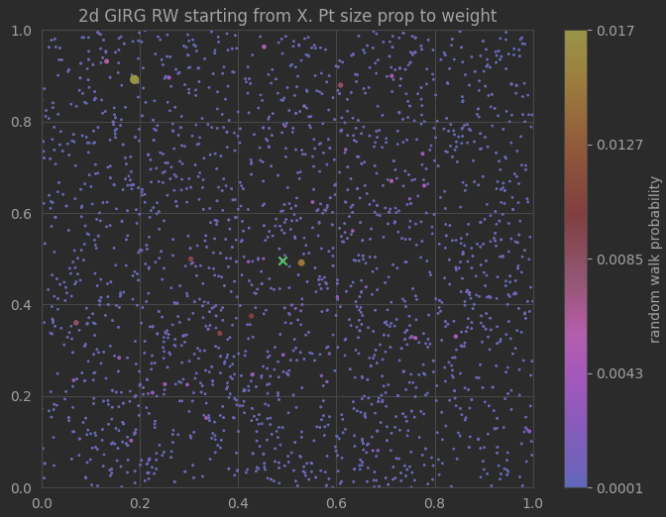
\includegraphics[width=\linewidth]{figures/2d_GIRG_RW.png}
    \caption{Naive approach: Large weight nodes (drawn with larger radii) get disproportionately more probability mass.}
  \end{subfigure}
  \hfill
  \begin{subfigure}{0.49\textwidth}
    \centering
    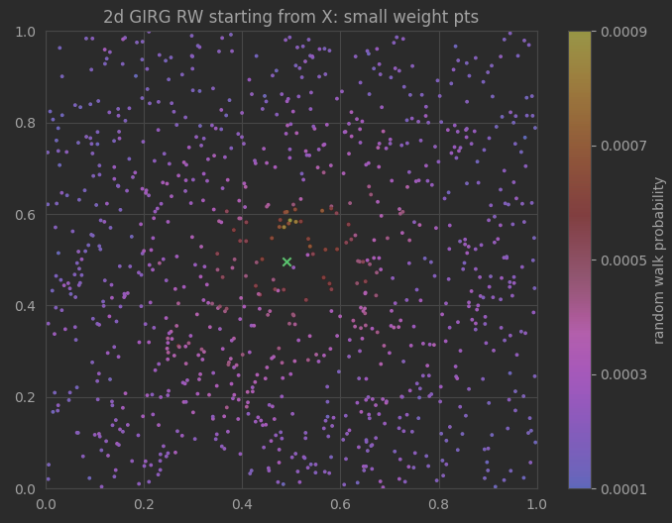
\includegraphics[width=\linewidth]{figures/2d_GIRG_RW_small_weights.png}
    \caption{Restriction of previous plot to nodes with smaller weights. Probability distribution looks more gaussian}
  \end{subfigure}

  \vspace{1em}

  \begin{subfigure}{0.49\textwidth}
    \centering
    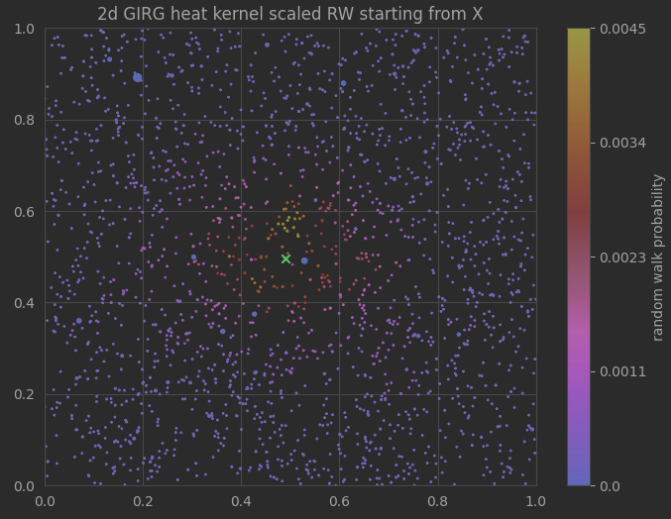
\includegraphics[width=\linewidth]{figures/2d_GIRG_heatkernelscaled_RW.png}
    \caption{Heat Kernel scaled edge weights using expected distance $W_{uv} = e^{-\hat{r}_{uv}^2}$. Helps to remove the large weight bias - perhaps a little too much.}
  \end{subfigure}
  \hfill
  \begin{subfigure}{0.49\textwidth}
    \centering
    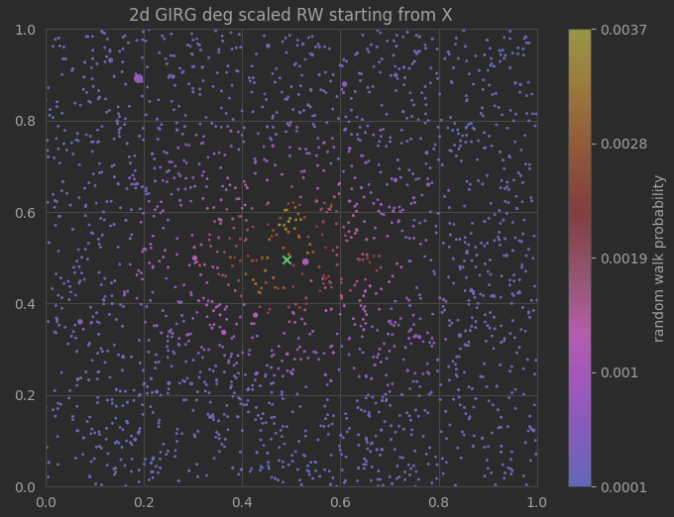
\includegraphics[width=\linewidth]{figures/2d_GIRG_degscaled_RW.png}
    \caption{Scaling transition probabilities by node degree $d_i^{-1}$  also removes the large weight bias.}
    \label{fig:diffmap_algo_comparisons_degscaled}
  \end{subfigure}
  \caption{6 step random walk diffusion cloud starting at the node marked with the green x, for three different (weightings) transition probability schemes. Graph generated from a 2d torus GIRG, whose true point locations give x and y axis.}
  \label{fig:diffmap_algo_comparisons}
  % \caption{Diffusion map eigenvalues (including $\lambda_1 = 1$) for a $n=2000, \tau=2.5, \alpha=1.3$ Cube GIRG with $d=1,2,3,4$ dimensions.}
  % \label{fig:cube_diffmaps_d1to4_evals}
\end{figure}



% % 
% The m-truncated diffusion map representation becomes the new r epresentation of nodes in the graph. The diffusion map is then a function $\R^n \to \R^m$. The first coordinate $\lambda_1$ is always $1$, corresponding to the stationary distribution of the random walk which all node diffusion maps converge to. This is useless for differentiating nodes and is hence dropped.

% Notably the transition matrix satisfies $M1 = 1$ since $\sum_j \frac{w_{ij}}{\deg(i)} = 1$, and it can be shown that it has eigenvalues $\lambda_1=1 \geq \lambda_2 \geq \lambda_3 \geq ...$.  





% Oh no $\vec{x}$.

% by the transition matrix $M = D^{-1}W$, where $D$ is the diagonal matrix with $D_{uu} = \sum_{v\in V} W_{uv}$ is the diagonal degree matrix, and $W_{uv}$ is the adjacency matrix, $W_{uv} = \begin{cases}1 & u \sim v \\0 & u \nsim v \end{cases}$. The matrix $S = D^{-1/2} W D^{-1/2}$ is a symmetrised version and hence is diagonalisable as $S = V \Lambda V^T$. Then the map $M = D^{-1/2} S D^{1/2} = D^{-1/2} V \Lambda (D^{1/2} V)^T = \Phi \Lambda \Psi^T$.

% In particular, starting at node $i$ (numbered $i=1,...,n$), the $t$th step diffusion cloud is $i \mapsto M^t_{ij} = (\Phi \Lambda^t \Psi^T)_{ij} = \sum_{k=1}^n \Phi_{ik} \lambda_k^t \Psi_{jk}$.

% So writing $\Phi = [\phi_1, \phi_2, ..., \phi_n]$ and $\Psi = [\psi_1, \psi_2, ..., \psi_n]$, we have that the $t$th step diffusion cloud is $i \mapsto \sum_{k=1}^n \phi_k(i) \lambda_k^t \vec{\psi}_k$. I.e. the diffusion map coordinate system is $\text{diffmap}_t(i) = (\lambda_2^t \phi_2(i), \lambda_3^t \phi_3(i), ..., \lambda_{d+1}^t \phi_{d+1}(i))$. The first coordinate is always $1$, it's the stationary distribution that all diffusion clouds converge to, so is discarded.

\section{Rescaling Points and Empirical Results}
If we have a graph $G$ which we know is generated from a $d$-dimensional GIRG, we can simply extract the $d$-truncated diffusion map coordinates of each node as an initial estimate for the original geometric location of the node. From \cref{sec:diff_map_geometry} we know the embedding should be roughly isometric up to a scale factor - so rescaling and shifting into the unit cube/torus is a first good step to make inter-point distances meaningful (even though this could be absorbed into the probability scaling constant $c$). There are also some other post processing steps that can be done to improve fit for real graphs.

\subsection{Inferring dimension $d$}
A first question is to choose the output dimension $d$ (truncation for the embedding) of the diffusion map, if the true geometric dimension $d$ of the input graph $G$ is unknown.

Diffusion maps actually present one way to infer the dimensionality by analysing the ordered sequence of eigenvalues $\lambda_2 < \lambda_3 < ...$. For example in \cref{fig:cube_diffmaps_d1to4_evals} we see that for graphs generated from cube GIRGs with dimension $d=1,2,3,4$, the diffusion map eigenvalue have a clear cutoff point after the first $d+1$ eigenvalues, with $\lambda_2, ..., \lambda_{d+1}$ being all approximately equal. Hence an eigenvalue cutoff can be used to infer geometric dimensionality of a graph - unfortunately messier real world graphs may not be so clear cut.

TODO plot some real graph eigenvalue plots?

% If there is a good cutoff point whereby the first $d$ eigenvalues are of similar large size, and the rest are much smaller, . This indeed works well for graphs synthetically generated from GIRGs, not so well on real world graphs.



\begin{figure}
  \centering

  \begin{subfigure}{0.49\textwidth}
    \centering
    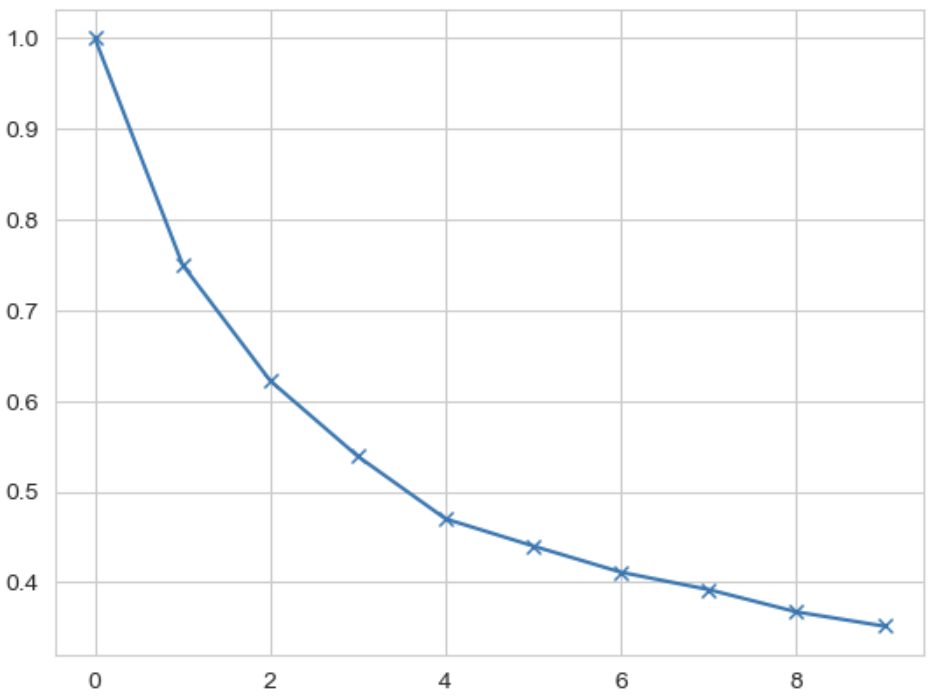
\includegraphics[width=\linewidth]{figures/diffmap_1d.png}
    \caption{$d=1$}
  \end{subfigure}
  \hfill
  \begin{subfigure}{0.49\textwidth}
    \centering
    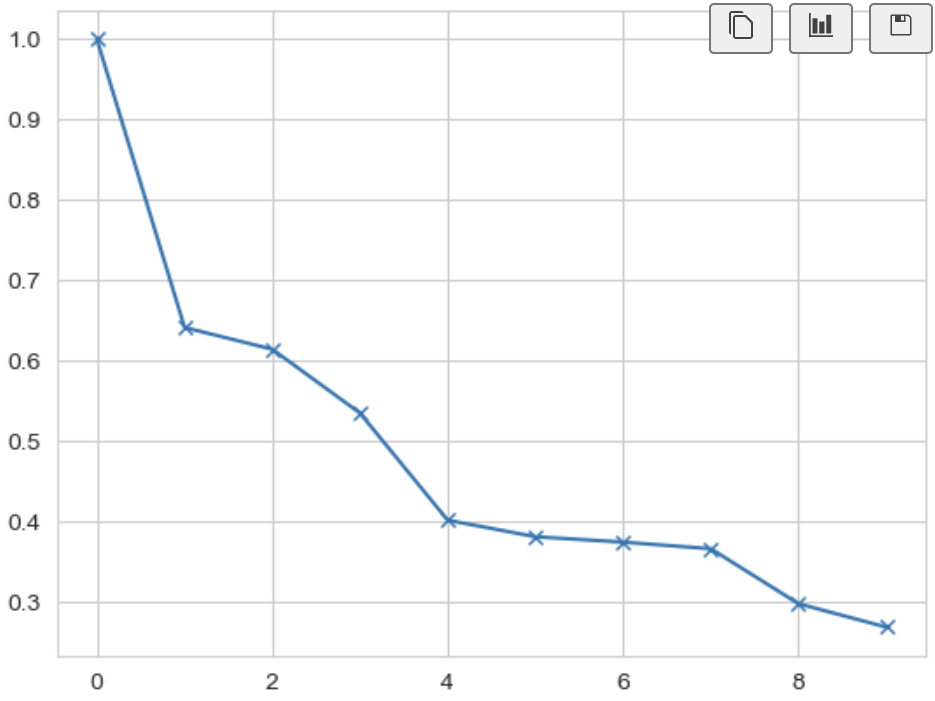
\includegraphics[width=\linewidth]{figures/diffmap_2d.png}
    \caption{$d=2$}
  \end{subfigure}

  \vspace{1em}

  \begin{subfigure}{0.49\textwidth}
    \centering
    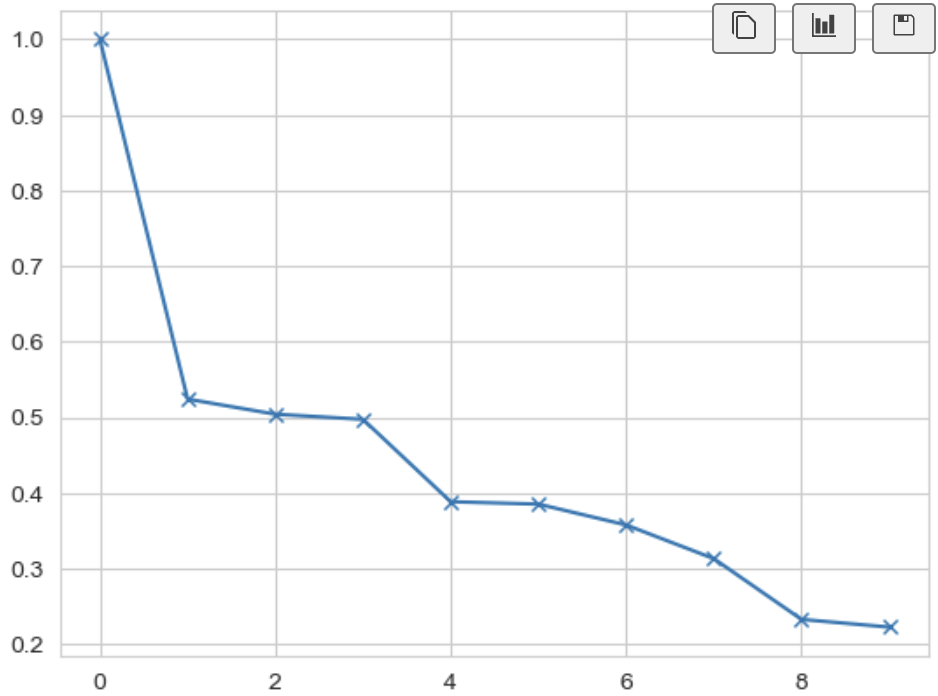
\includegraphics[width=\linewidth]{figures/diffmap_3d.png}
    \caption{$d=3$}
  \end{subfigure}
  \hfill
  \begin{subfigure}{0.49\textwidth}
    \centering
    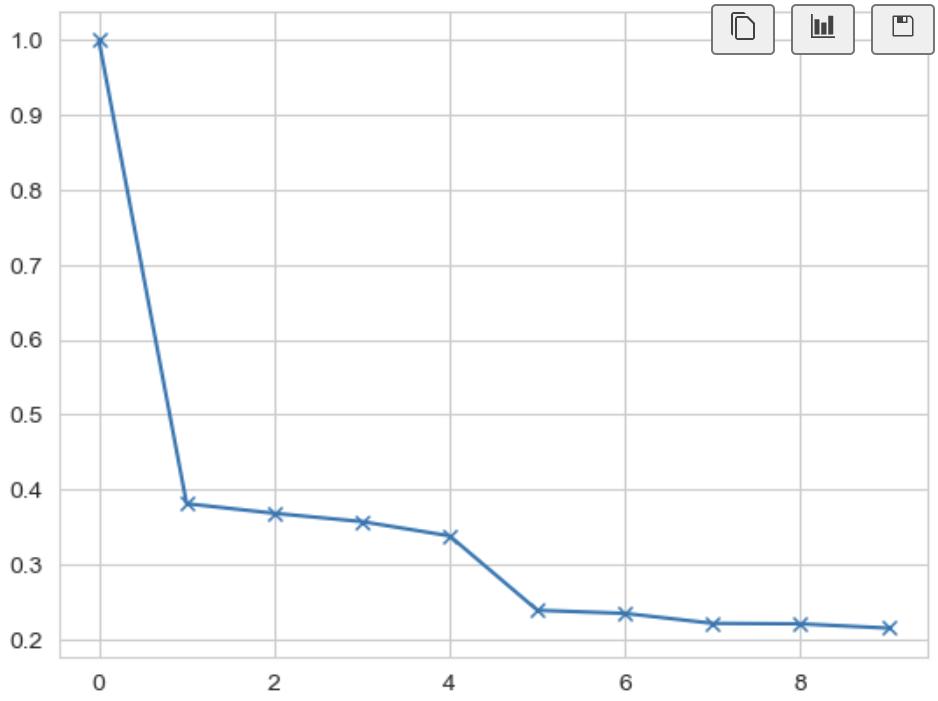
\includegraphics[width=\linewidth]{figures/diffmap_4d.png}
    \caption{$d=4$}
    \label{fig:cube_diffmaps_d4}
  \end{subfigure}

  \caption{Diffusion map eigenvalues (including $\lambda_1 = 1$) for a $n=2000, \tau=2.5, \alpha=1.3$ Cube GIRG with $d=1,2,3,4$ dimensions.}
  \label{fig:cube_diffmaps_d1to4_evals}
\end{figure}
\subsection{Rescaling/Shifting Diffusion Maps}
We see in \cref{fig:cube_diffmap_plots_d1and2} some raw $d=2$ truncated diffusion maps. When the underlying graph was a 2d square GIRG, the inferred points look indeed square like, whereas from a 1d GIRG we do at least get a (curved) line in 2d space.


In general the points will be centered around the origin, as all $\lambda_2, \lambda_3, ...$ eigenvalue eigenvectors will be orthogonal to the stationary distribution $\vec{\phi}_1 = k \vec{1}$ : they represent a deviation from the stationary distribution - e.g. for a node on the 1D line towards left end, it will need to put more diffusion probability on the left side nodes, and less on the right side nodes than the stationary distribution. The y-axis scale is small as $\lambda_2 < 1$, and is decreasing with $t$.


The 0 centering can easily be fixed to be more cube GIRG like by shifting the points $(\vec{x}_u)_i \gets (\vec{x}_u)_i + \min_v (\vec{x}_v)_i$.
If we are certain that the points should be distributed within the unit cube, then we can simply rescale separately along each dimension: $x \gets \frac{x - x_{\min}}{x_{\max} - x_{\min}}$.
If furthermore we're certain that the distribution within the unit cube should be relatively uniform, we can perform a coordinatewise "uniformify" procedure that replaces $(\vec{x}_u)_i$ with its percentile value compared with other $(\vec{x}_v)_i$. \cref{fig:diffmap_uniformed_vs_nonuniformed} shows the "uniformify" procedure in action. This helps to counteract the phenomenon of terribly different diffusion map scaling, whereby the majority of the graph which is well connected ends up highly bunched up, and a small number of outlying poorly connected nodes cover most of the embedding space. 

% Notably on real graphs where the truncated diff map coordinates are not guaranteed to be independently distributed, coordinatewise percentile mapping can lead to slightly odd results - see socfb-Amherst where there's a strong $x_1 = 1 - x_2$ correlation for small $x_1$. It's still a good improvement over the original non rescaled diffusion map.

% The decreasing diffusion map scaling can be see either as a bug or a feature. If we are certain that the points should be distributed within the unit cube, then we can simply rescale separately along each dimension: $x \gets \frac{x - x_{\min}}{x_{\max} - x_{\min}}$. If furthermore we're certain that the distribution within the unit cube should be relatively uniform, we can perform a coordinatewise "uniformify" procedure that replaces $(x_u)_i$ with its percentile value compared with other $(x_v)_i$. \cref{fig:diffmap_uniformed_vs_nonuniformed} shows the "uniformify" procedure in action. Notably on real graphs where the truncated diff map coordinates are not guaranteed to be independently distributed, coordinatewise percentile mapping can lead to slightly odd results - see socfb-Amherst where there's a strong $x_1 = 1 - x_2$ correlation for small $x_1$. It's still a good improvement over the original non rescaled diffusion map. 

% Critically since there is no guarantee that the scaling of diffusion map coordinates is the same as the original GIRG coordinates, using some kind of prior knowledge to rescale the diffusion map is important to yield geometric information with meaningful inter-point distances.

\begin{figure}
  \centering

  \begin{subfigure}{0.49\textwidth}
    \centering
    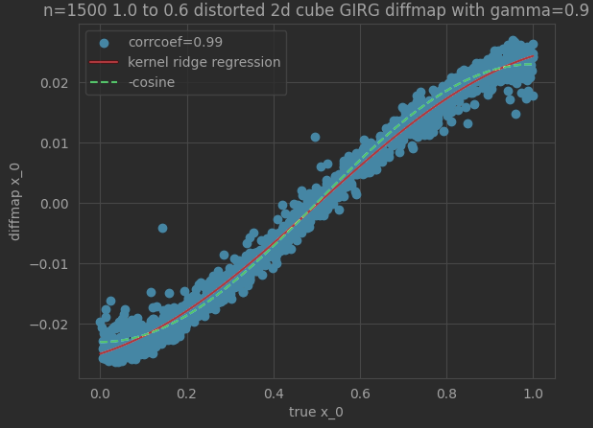
\includegraphics[width=\linewidth]{figures/2d_distorted_diffmap_plot_major.png}
    \caption{$d=1$}
    \label{fig:2d_distorted_major}
  \end{subfigure}
  \hfill
  \begin{subfigure}{0.49\textwidth}
    \centering
    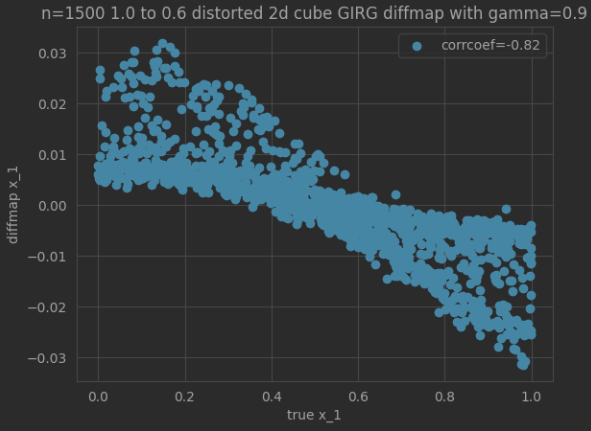
\includegraphics[width=\linewidth]{figures/2d_distorted_diffmap_plot_minor.png}
    \caption{$d=2$}
    \label{fig:2d_distorted_minor}
  \end{subfigure}


  \caption{Major and minor diff map against real}
  \label{fig:2d_distorted_major_minor}
\end{figure}


\paragraph{Rotated Points} One issue with diffusion maps as seen in \cref{fig:cube_diffmap_plots_d2}, the 2D GIRG's 2D-truncated diff map looks like a rotated square. While the diffusion map has successfully extracted geometric information from the graph, it's not done so in the original basis. This phenomenon can make rescaling/uniformifying to the unit cube a little questionable. 

One possible explanation is that as diffusion map is trying to maximise diffusion explainability, the long square diagonal has overall more diffusion along it. This is not very convincing though as there would then be less diffusion in the opposite corners. Even assuming no overall rotation bias, you're going to get a square rotated somewhere between $0$ and $45$ degrees.

\paragraph{Cuboidal (non-cube) GIRGs} However in practice, real graphs never have an equal balance in geometric dimension importance. This is easiest to understand with the example of a weighted euclidean norm setup, where it could be that a 2D GIRG's true 1st geometric dimension (between $[0, 1]$) is more important than its 2nd geometric dimension in influencing edge probabilities: $\norm{x - y} = \sqrt{a (x_1 - y_1)^2 + b(x_2 - y_2)^2}$.
The diffusion map is solving an eigenvalue problem that is like a maximsation of diffusion explainability. If $a > b$, then by maximisation the first diffusion map coordinate $\varphi_1(u)$ is likely to be very similar to $(\vec{x}_u)_1$. Only if $a=b$ is there no preference between $(\vec{x}_u)_1$ and $(\vec{x}_u)_2$, making a rotation possible.
Hence the points $(\varphi_1(u), \varphi_2(u))_{u \in V}$ are likely to end up as a rectangle, not a rotated square; the variation in first coordinate will be greater than in the second.

\cref{fig:2d_distorted_major} shows the 2d diff map embedding of such a distorted 2d cube GIRG. Note that the major coordinate is much easier to fit well, whereas the minor one has higher error (NB the diff map embedding of $x_2$ is negatively scaling with the true value which is fine - we can never guarantee same signs).
We also see that the $x_1$ diffusion map embedding doesn't have quite a linear relationship with the real locations - it looks more like a cosin wave like relationship - this actually makes sense as eigenfunctions of the laplacian operator on a cube look like sine waves.


In the light of potentially non equal coordinates, the relative $\lambda_2 > \lambda_3 > ...$ scaling can be seen as a feature not a bug, if the hypothesis space of generative graph models is to be expanded to cuboid (non-cube) GIRGs. In this case all coordinates of the diffusion map don't have to be all (non-homogeneously) rescaled to the range $[0, 1]$ and can rather be homogeneously rescaled to retain their relative size ratios.
This sheds new light on the horizontalness of the $\lambda_2, \lambda_3, \lambda_4, \lambda_5$ line segment in \cref{fig:cube_diffmaps_d4} as a testament to the underlying cube (non cuboid) GIRG that generated the graph.




% In this case, the diffusion map coordinates will have a larger scale for the $\lambda_2$ coordinate than the $\lambda_3$ coordinate, and the points will look like an elongated rectangle.

% the distance: $\norm{x - y} = \sqrt{a (x_1 - y_1)^2 + b(x_2 - y_2)^2}$. In this case, the diffusion map coordinates will have a larger scale for the $\lambda_2$ coordinate than the $\lambda_3$ coordinate, and the points will look like an elongated rectangle. The flatness of $\lambda_2, \lambda_3, \lambda_4, \lambda_5$ line segment in \cref{fig:cube_diffmaps_d4} is a testament to the cube (and non cuboidness) of the underlying GIRG that generated the graph.


% (relatively uniformly) distributed within the unit cube, then we can simply rescale separately along each dimension.
% A linear coordinatewise scaling $x \gets \frac{x - x_{\min}}{x_{\max} - x_{\min}}$ works, or more extremely a coordinatewise "uniformify" procedure that replaces $(x_u)_i$ with its percentile value compared with other $(x_v)_i$.
% In \cref{fig:diffmap_uniformed_vs_nonuniformed} we see uniformified versions of a generated 2D GIRG, and the socfb-Amherst41 graph.

% Seen as a feature, the relatively different scaling allows as a natural correction to the potential non equivalence of different dimensions. For instance in a weighted euclidean norm setup, it could be that a 2D GIRG's true 1st geometric dimension (between $[0, 1]$) is much more important than its 2nd geometric dimension in determining the distance: $\norm{x - y} = \sqrt{a (x_1 - y_1)^2 + b(x_2 - y_2)^2}$. In this case, the diffusion map coordinates will have a larger scale for the $\lambda_2$ coordinate than the $\lambda_3$ coordinate, and the points will look like an elongated rectangle. The flatness of $\lambda_2, \lambda_3, \lambda_4, \lambda_5$ line segment in \cref{fig:cube_diffmaps_d4} is a testament to the cube (and non cuboidness) of the underlying GIRG that generated the graph. 


% TODO put in some eigenvalue plots

\begin{figure}
    \centering

    \begin{subfigure}{0.49\textwidth}
      \centering
      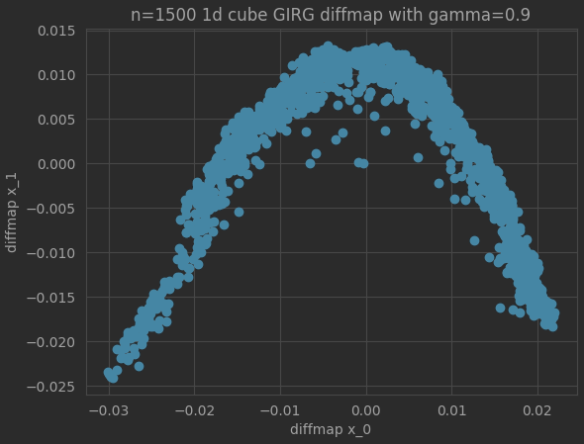
\includegraphics[width=\linewidth]{figures/1d_GIRG_diffmap.png}
      \caption{$d=1$}
      \label{fig:sub1}
    \end{subfigure}
    \hfill
    \begin{subfigure}{0.49\textwidth}
      \centering
      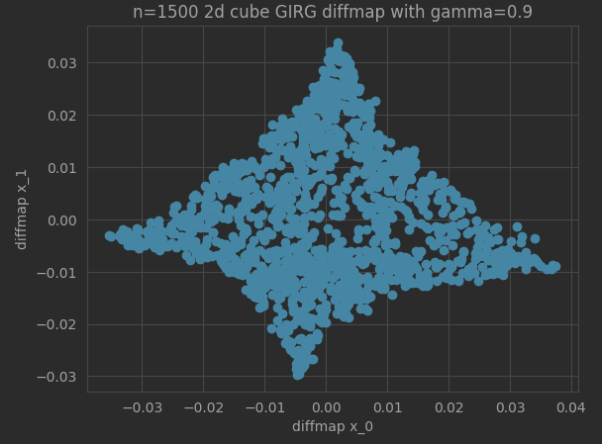
\includegraphics[width=\linewidth]{figures/2d_GIRG_diffmap.png}
      \caption{$d=2$}
      \label{fig:cube_diffmap_plots_d2}
    \end{subfigure}

  
    \caption{Diffusion map scatter plot of the first two extracted coordinates from 1d and 2d GIRGs.}
    \label{fig:cube_diffmap_plots_d1and2}
\end{figure}


\begin{figure}
    \centering

    \begin{subfigure}{0.49\textwidth}
      \centering
      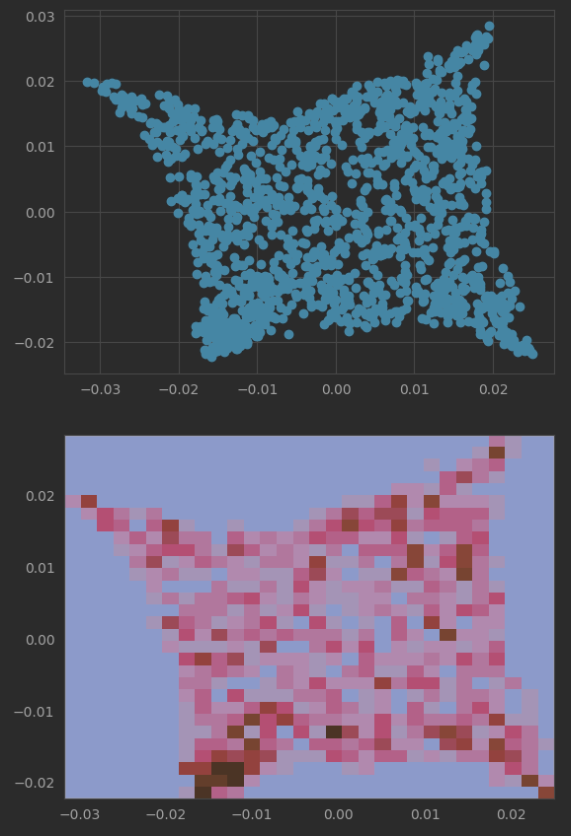
\includegraphics[width=\linewidth]{figures/diffmap_plot_nonuniformed.png}
      \caption{2d GIRG non-uniformed}
      \label{fig:sub1}
    \end{subfigure}
    \hfill
    \begin{subfigure}{0.49\textwidth}
      \centering
      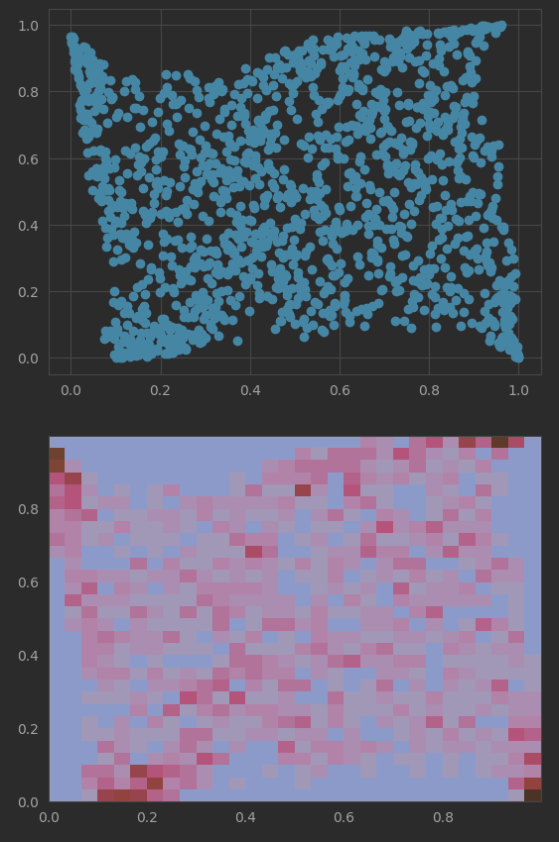
\includegraphics[width=\linewidth]{figures/diffmap_plot_uniformed.png}
      \caption{2d GIRG uniformed}
      \label{fig:sub2}
    \end{subfigure}
  
    \vspace{1em}
  
    \begin{subfigure}{0.49\textwidth}
      \centering
      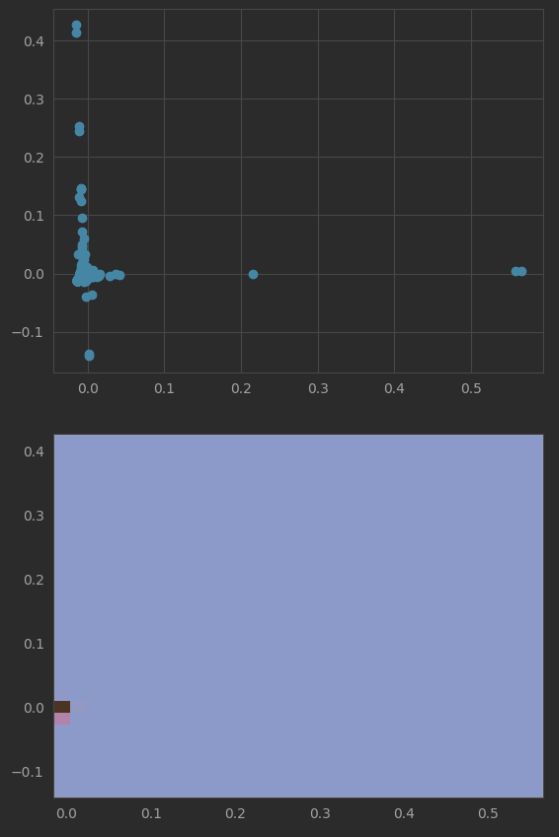
\includegraphics[width=\linewidth]{figures/real_diffmap_plot_nonuniformed.png}
      \caption{socfb-Amherst41 non-uniformed}
      \label{fig:sub3}
    \end{subfigure}
    \hfill
    \begin{subfigure}{0.49\textwidth}
      \centering
      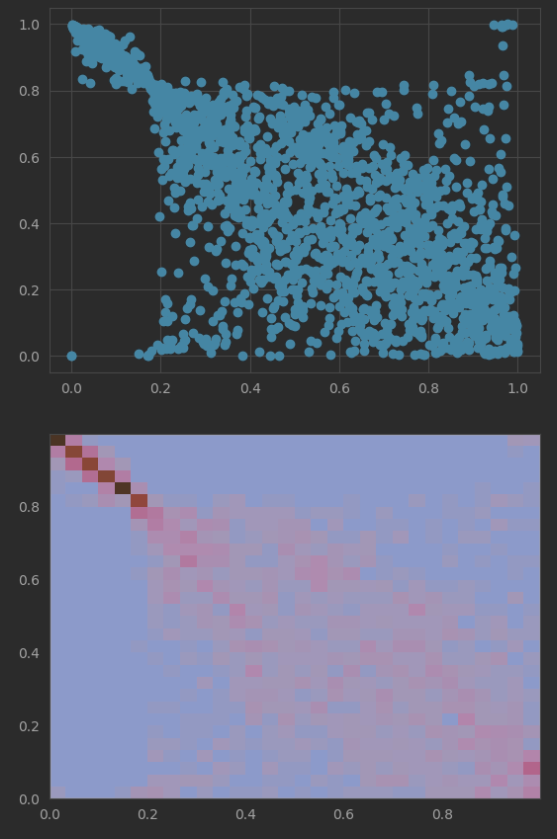
\includegraphics[width=\linewidth]{figures/real_diffmap_plot_uniformed.png}
      \caption{socfb-Amherst41 uniformed}
      \label{fig:sub4}
    \end{subfigure}
  
    \caption{Diffusion map scatter plot of the first two extracted coordinates, with and without using an additional uniform square remapping}
    \label{fig:diffmap_uniformed_vs_nonuniformed}
\end{figure}


% \begin{figure}
%   \centering

%   \begin{subfigure}{\textwidth}
%     \centering
%     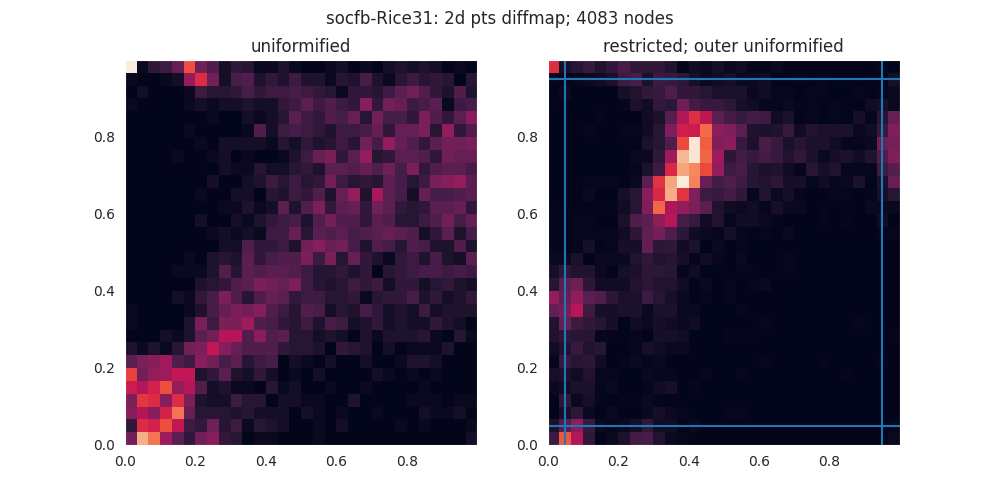
\includegraphics[width=\linewidth]{figures/socfb-Rice31_2ddiffmap_unif_vs_restrict.png}
%     % \label{fig:sub1}
%   \end{subfigure}

%   \vspace{1em}
%   \begin{subfigure}{\textwidth}
%     \centering
%     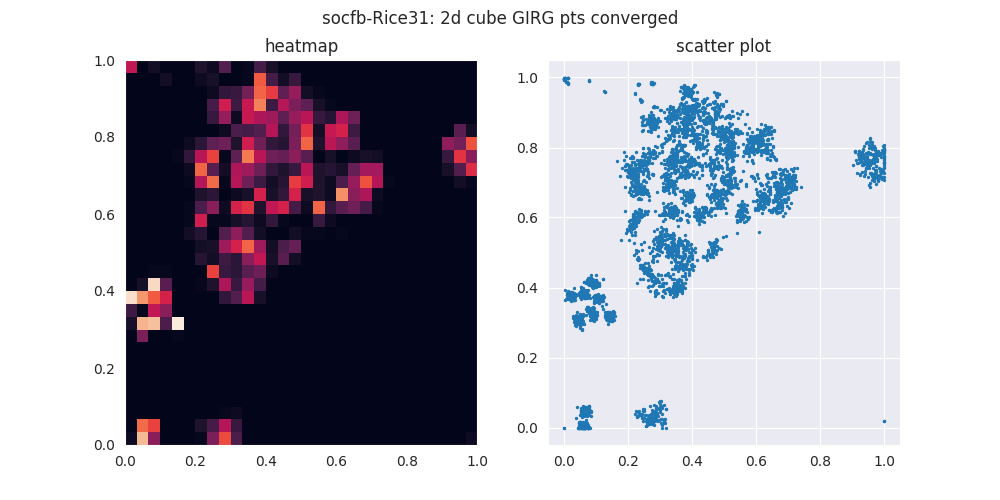
\includegraphics[width=\linewidth]{figures/socfb-Rice31_2d_cube_GIRG_converged.png}
%     % \label{fig:sub1}
%   \end{subfigure}

%   \vspace{1em}
  
% \end{figure}
% \begin{figure}
%   \begin{subfigure}{\textwidth}
%     \centering
%     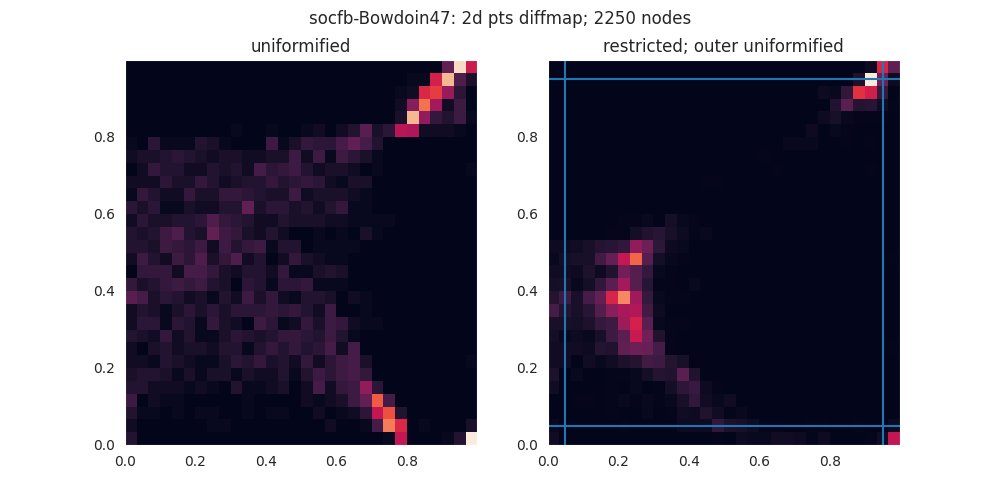
\includegraphics[width=\linewidth]{figures/socfb-Bowdoin47_2ddiffmap_unif_vs_restrict.png}
%     % \label{fig:sub1}
%   \end{subfigure}

%   \vspace{1em}
%   \begin{subfigure}{\textwidth}
%     \centering
%     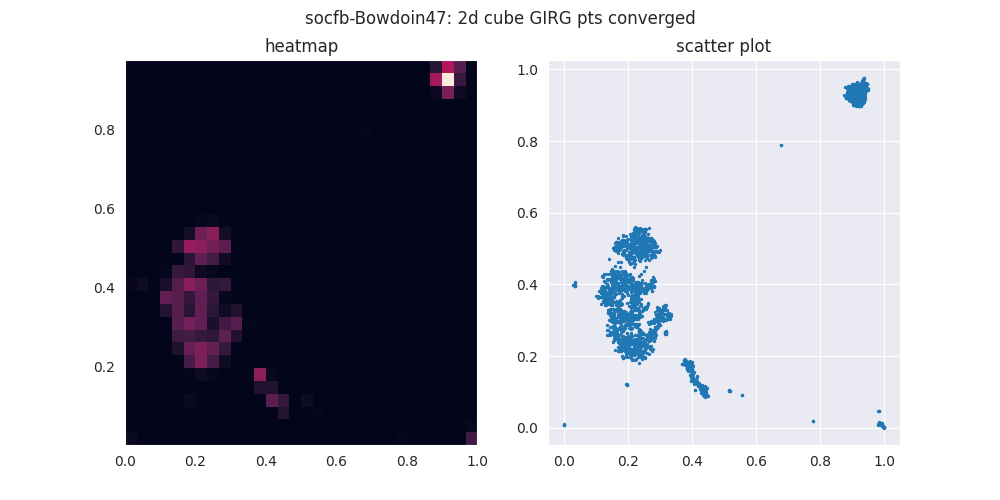
\includegraphics[width=\linewidth]{figures/socfb-Bowdoin47_2d_cube_GIRG_converged.png}
%     % \label{fig:sub1}
%   \end{subfigure}

% \end{figure}


% \begin{figure}
%   \begin{subfigure}{\textwidth}
%     \centering
%     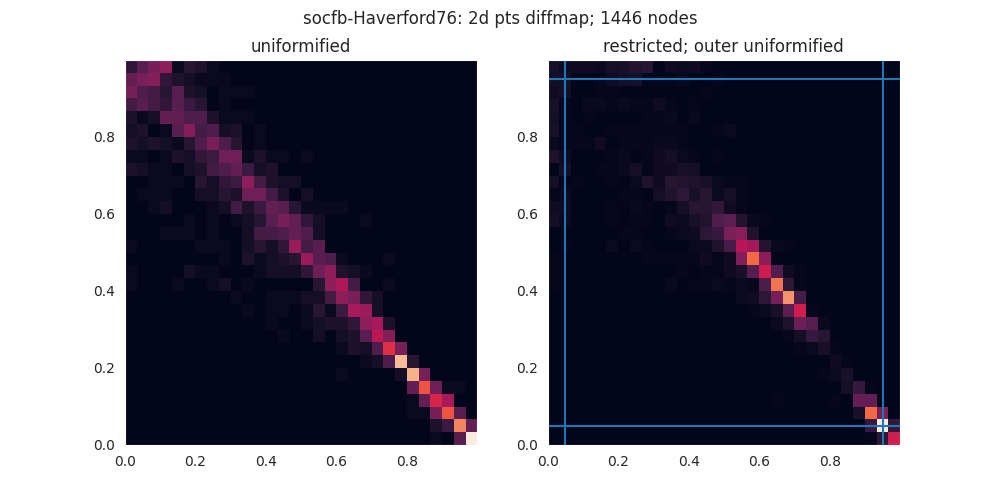
\includegraphics[width=\linewidth]{figures/socfb-Haverford76_2ddiffmap_unif_vs_restrict.png}
%     % \label{fig:sub1}
%   \end{subfigure}

%   \vspace{1em}
%   \begin{subfigure}{\textwidth}
%     \centering
%     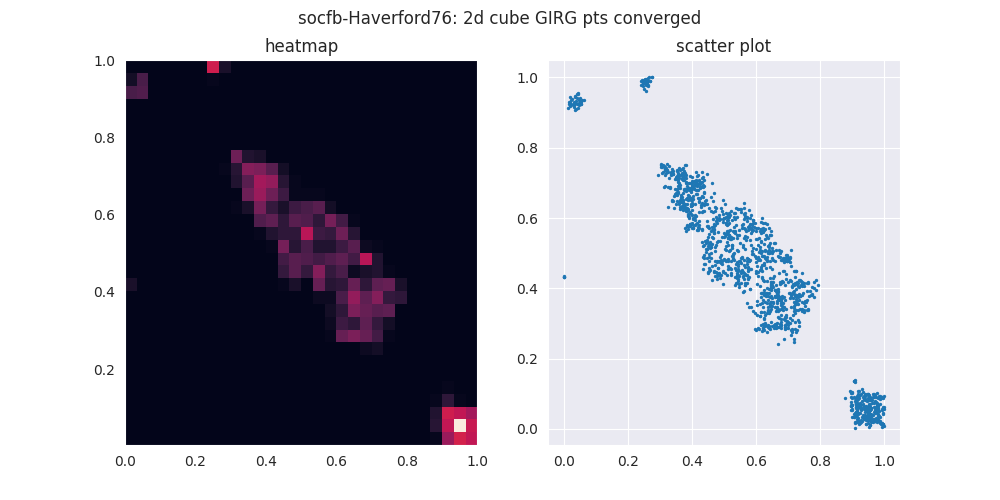
\includegraphics[width=\linewidth]{figures/socfb-Haverford76_2d_cube_GIRG_converged.png}
%     % \label{fig:sub1}
%   \end{subfigure}


%   \caption{two methods for rescaling/shifting diffusion maps into the cube - done here for d=2 truncations. The blue lines for the restricted version show the border at which points are outer uniformified.}
%   \label{fig:uniformifed_vs_restricted_rescaling}
% \end{figure}


\begin{figure}
  \begin{subfigure}{0.47\textwidth}
    \centering
    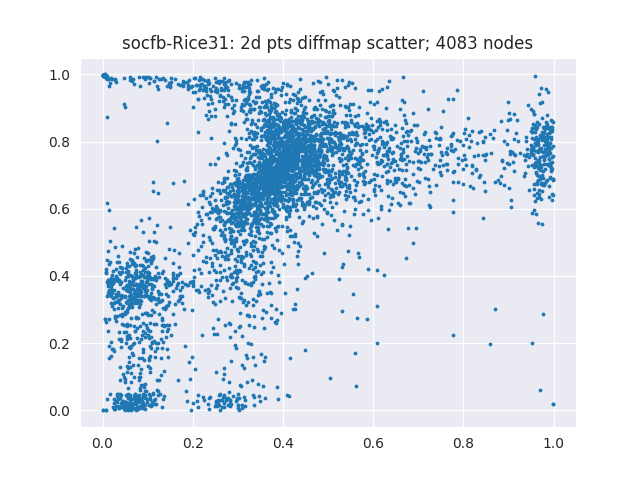
\includegraphics[width=\linewidth]{figures/socfb-Rice31_2ddiffmap_restrict_scatter.png}
    % \label{fig:sub1}
  \end{subfigure}
  \hfill
  \begin{subfigure}{0.47\textwidth}
    \centering
    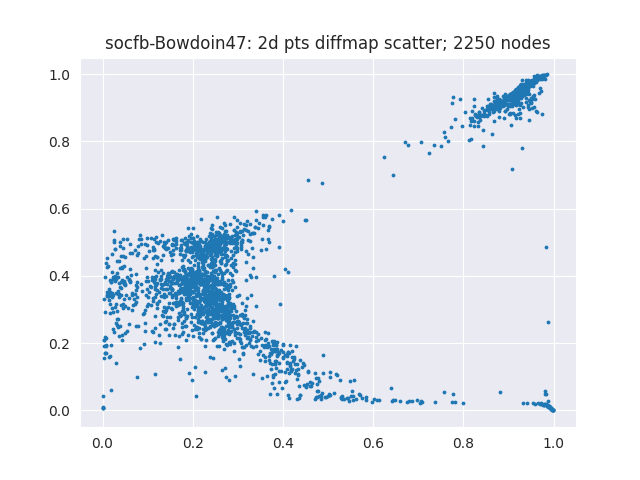
\includegraphics[width=\linewidth]{figures/socfb-Bowdoin47_2ddiffmap_restrict_scatter.png}
    % \label{fig:sub1}
  \end{subfigure}


  \caption{the diffmaps (here 2d, restricted and outer uniformified) don't have much point clustering - it's more higher diffusion level than caring so much about individual edges like in the converged case}
  \label{fig:uniformifed_vs_restricted_rescaling}
\end{figure}



\paragraph{Toroidal GIRGs} Interestingly Toroidal GIRGs are differentiated from Cube GIRGs in that the diffusion map requires $2d$ coordinates to capture the Torus geometry instead of just $d$ for the cube. The natural diffusion map of a 1D Torus GIRG ends up being a 2D circle about the origin; 2 larger eigenvalues $\lambda_2, \lambda_3$ are necessary. 


% A final issue with diffusion maps is that points seem to end up concentrated in corners/edges. My hypothesis is that this is because e.g. on a 1D line segment, it's hard to distinguish somewhat left and very left points - in the end the diffusion cloud bias is still just left leaning. Not sure how much of a problem this is.

\paragraph{Restricted Rescaling} This method works to bias less towards a uniformly distributed prior while still mapping points into a reasonable geometric space.
Empirically, the diffusion map coordinates of the facebook graphs often have $\geq 90\%$ of the nodes concentrated in a small parcel, with only a few nodes having extremely far out locations.
This defeats the simple rescaling method of $x \gets \frac{x - x_{\min}}{x_{\max} - x_{\min}}$ as most nodes will end up very tightly packed - however if we hit all the points with a uniformify procedure hammer, we will lose the more subtle geometry picked up by the diffusion map within the highly connected central parcel.

Instead we only rescale the central nodes: those whose joint coordinate-wise percentiles lie in $[5\%, 95\%]^d$.
These nodes are linearly scaled to the $[0.05, 0.95]^d$ cube. Finally the outlying nodes are percentile rescaled (non-linearly) to the upper/lower cube margins.
This method is shown in comparison for a few graphs in \cref{fig:uniformifed_vs_restricted_rescaling}


TODO 

- fuller analysis of different diffmap modes: 'uniformify', 'cubify' and 'cuboidify', comparing performance on real life and synthetic graphs

- presentation of the small degree stochastic walk tweak which improves diffusion map performance:
\begin{verbatim}
# Empirically this gamma seems to work well. 
# It discourages taking edges to popular nhbs.
gamma = 0.9
M_tilde = scipy.sparse.diags(1 / D) @ A @ scipy.sparse.diags(D ** (-gamma))
M_tilde = scipy.sparse.diags(np.array(1 / M_tilde.sum(axis=-1)).squeeze()) @ M_tild
\end{verbatim}

- is it true that diffusion map tends to cluster representations edges rather than being more uniform? Empricially seems to happen in 2D but not 1D?


\chapter{MCMC}
\section{Introduction}
The binary classification framework is designed to compare the similarity of two distributions of datapoints. Each graph is a datapoint, and the classifier compares graphs only on higher level features meant to distinguish distributions of graphs, not individual graphs. In particuular these features are node permutation invariant - such as average degree, effective diameter and so on.

An alternative framework is to try to fit a GGM model to a graph so as to compare on an edgewise and likelihood basis. For for the GIRG GGM, this means not just fitting $\hat{\alpha}$ to match the local clustering coefficient, $\hat{c}$ to match the number of edges, and $\hat{\tau}$ to match the degree distribution tail, but to further actually try and infer individual node weights $w_u$, and positions $x_u$. 

We saw this already to some extent with the copy-weight GIRGs - where $\hat{w}_u = d_u$ is fit, as the observed real graph node degrees. The $x_u$ are much harder to fit - for a start any maximum likelihood fit $\hat{x}_u$ would be rotation, reflection, and translation invariant (isometries). Finding any one maximum likelihood fit is impractical for all but the smallest graphs. Instead we try a Markov-Chain MonteCarlo (MCMC) approach to sample a set of locations $\{x_u\}$ from the posterior distribution.

\section{Formulation}
MCMC is a method in the bayesian framework of a parametric generative model. Parameter $\theta$ has prior $p(\theta)$. Datapoint $z \sim p(z | \theta)$. In our case of our node specific fitting GIRG GGM, $\theta = (\alpha, c, \{w_u\}_{u \in V}, \{x_u\}_{u \in V})$, and we focus in particular on the locations $x_u$. $z$ for us is one real graph instance $G$.

The posterior likelihood $p(\theta | z) = \frac{p(z | \theta) p(\theta)}{p(z)}$ is infeasible to compute due to the normalising factor $p(z)$. MCMC instead uses the non normalised $Q(\theta) = p(z | \theta) p(\theta)$ which can be evaluated, to set up a Markov Chain with states $\theta \in \Theta$, and transition probabilities derived from $Q(\theta)$. In particular we will use a Metropolis-Hastings style markov chain. With a proper MC state transition probability $p(\theta \to \theta')$, we can perform a random walk on the MC state space that converges in the limit to the posterior distribution $\theta \sim p(\theta | z)$. If the jth step of the random walk yields $\theta^j$, given sufficient burn in and spacing, we can sample $\theta^{j_1}, \theta^{j_2}, ...$ from the posterior. We will be content with just one posterior sampled $\hat{\theta}$ (NB not a maximum likelihood estimator), and use this to evaluate our overall GIRG model fit to the real graph.

I think we do a Gibb's sampling approach. This means both breaking down $\theta$ into subcomponents $\theta_i$, randomly choosing one to propose a new state for, i.e. $\theta' = (\theta'_i, \theta_{-i})$, and using the $Q_i(\theta_i)$ instead of $Q(\theta)$ - i.e. just the marginal non-normalised posterior. In our case $Q(\theta) = p(G | \theta) p(\theta)$, so the uniform prior $p(\theta)$ can be dropped everywhere as $p(\theta) = 1\; \forall \theta$, and then $p(G | \theta) = \prod{u, v \in V; u \neq v} p(e(u,v) | w_u, w_v, x_u, x_v, \alpha, c)$. This lends well to Gibb's sampling - we need concentrate only on $Q_u(\theta_u) = \prod{v \neq u} p(e(u,v) | ...)$.

Key elements of the MCMC approach are 1. burn in time, and 2. proposal distribution. 

Burn in time can be quite long. One key component is a good initialisition. With the GIRG model, the natural initialisation for $x_u$ would be to follow the prior $x_u \sim U([0, 1]^d)$. Instead we use an initialisation based on d-truncated diffusion map from the real graph connectivity. We also try to optimise our code and use multiprocessing to speed up the random walk.

The proposal distribution should be designed to maximise chances of acceptance. It seemed reasonable to stochastically propose either a small local perturbation, or a random jump to anywhere in the cube, with some probability of either (we elected for 70\% small perturbation). A random uniform jump is useful to try and find a completely new location for $x_u$ that could suit (hopefully near to its neighbours) - in fact another good proposal would be to randomly choose a neighbour $v \sim u$, and move $x_u$ to a random offset of $x_v$. A small perturbation $x_u' = x_u + \epsilon$ is good as assuming $x_u$ has high likelihood, somewhere nearby might have even higher.

\paragraph{Acceptance probability} in the Metropolis-Hasting's algorithm, this is 
\begin{align}
  A(x_u', x_u) &= \min \left (1,\;\;  \frac{p_{prop}(x_u | x_u') p(G | x_u') p(x_u')}{p_{prop}(x_u' | x_u) p(G | x_u) p(x_u)}\right )
  \\
  &= \min \left (1,\;\;  \frac{p(G | x_u')}{p(G | x_u)} \right )
  \\
  & \text{as $p_{prop}$ is symmetric and $p(x) = 1\; \forall x$}
\end{align}

\begin{comment}
\section{Bayes Factor likelihood comparisons}
\begin{enumerate}
    \item Using one MCMC posterior sample of $\{x_u\}_{u \in V}$ and maximum likelihood estimates $\hat{\alpha}, \hat{c}, \hat{w}_u$, we estimate the likelihood $p(\cG_{\GIRG} | G)$, and can perform a comaprison $p(\cG_{\GIRG-1d} | G)$ vs $p(\cG_{\GIRG}-2d | G)$ vs $p(\cG_{CL} | G)$ etc.
    \item Results show that $p(\cG_{\GIRG}-1d | G)$ is better than 2D, 3D GIRGs, but not as good as Chunglu
    \item Results show that simply introducing a failure rate of $0.5$ onto the GIRGs (unfortunately not correcting for LCC), the model probabiltiy estimate for 1D GIRG then beats out chunglu (all copyweights)
\end{enumerate}


What the heck is Bayes Factor anyway?

Apparently it's basically comparing $P(M_1 | D)$ and $P(M_2 | D)$. In our case $M_1, M_2$ is e.g. 1D GIRG vs 2D GIRG, and $D$ the data is just one graph instance. We have some prior of $P(M_1)$ vs $P(M_2)$, e.g. 50-50, or some kind of decaying $1D \GIRG > 2D \GIRG > 3D \GIRG > \dots$.

Then the comparison is $P(M_1 | D) = \frac{P(D | M_1) P(M_1)}{P(D)}$. I.e. the ratio $\frac{P(M_1 | D)}{P(M_2 | D)}$ is the ratio $\frac{P(D | M_1) P(M_1)}{P(D | M_2) P(M_2)}$.

We will ignore the priors $P(M_1), P(M_2)$, for now, and focus on the likelihoods $P(D | M_1), P(D | M_2)$. In our case if $M_1$ is a 1D GIRG, and we've decided to fix e.g. $\alpha, e, \{w_u\}_{u \in V}$, and just vary $\theta = c, \{x_u\}_{u \in V}$, then we could monte-carlo sample $\theta \sim p(\theta)$ from the prior to get an estimate, $P(D | M_1) = P(G) = \int_\theta P(G | \theta) p(\theta) d\theta$, where we drop the $| M_1$ as we've fix into the 1D GIRG universe.

This seems inefficient. Instead we can sample $\theta \sim P(\theta | G)$ from the posterior using MCMC, and then evaluate  

\begin{align*}
    1/P(G) 
        &= \int_\theta \frac{1}{P(G)} P(\theta) d\theta
        \\
        &= \int_\theta \frac{P(\theta, G)}{P(G)} \frac{1}{P(\theta, G)} P(\theta) d\theta 
        \\
        &= \int_\theta P(\theta | G) \frac{P(\theta)}{P(\theta, G)} d \theta
        \\
        &= \int_\theta P(\theta | G) \frac{1}{P(G | \theta)} d\theta
        \\
        &= E_{\theta \sim \theta | G} \left [ \frac{1}{P(G | \theta)} \right ]
        % &= \int_\theta P(\theta) P(G | \theta) d\theta
        % \\
        % &= \int_\theta P(\theta) \frac{P(\theta | G)}{P(\theta | G)} P(G | \theta) d\theta
        % \\
        % &= \int_\theta \frac{P(G, \theta)}{P(\theta | G)} P(\theta | G) d\theta
        % \\
        % &= \int_\theta \frac{P(G | \tehta) | \theta}
\end{align*}

The good news is that while MCMC sampling from $P(\theta | G)$, it seems that the likelihood $P(G | \theta)$ is relatively consistent.

TODO think through more penalisation of models by parameter count. Does this $P(G)$ calculation take this into account already? I.e. a high parameter count model can fit many different $G$, so although $G$ is more "plausible" under a higher count model, there are also more alternative outcomes $G'$ so as to dilute the probability?
\end{comment}

\section{Model Comparison}

We seek to show that the GIRG model does a better job at fitting the facebook graphs than the ChungLu model, which is the natural comparison point as essentially a GIRG without geometry. We would also like to determine between 1D, 2D etc. GIRGs what is the best dimensionality.

\subsection{Likelihood comparison of GIRG vs CL fit to real graph}
As a first sanity check, we can sample a $\hat{\theta}_{\GIRG}$ (not MLE but still pretty good) as from the posterior $\theta_{\GIRG} | G$ with MCMC, and more simply fit a $\hat{\theta}_{CL}$. Given that the 1D GIRG is a more parametrised model, it would be total failure if it didn't reproduce the given graph better. For most of the facebook graphs however, $p(G | \hat{\theta}_{\GIRG}, \cG_{\GIRG}) < p(G | \hat{\theta}_{CL}, \cG_{CL})$!
The GIRG model is far too confident about edges, giving $p_{uv} \approxeq 1$ for small $\norm{x_u - x_v}$ and $p_{uv} \approxeq 0$ for large $\norm{x_u - x_v}$. Hence a mistake on a few edges can lead to a large penalisation in likelihood. The ChungLu model is much more forgiving, with all probabilities more medium sized. 

One reasonable tweak is to introduce a failure rate $0 \leq f \leq 1$ to the GIRG model: 
% $p_{uv} = (1-f) \min( ... )$
\begin{equation}
  p_{uv} = (1 - f) \min \left \{ 
    1,
    c \left (
        \frac{w_u w_v / W}{\norm{x_u - x_v}^d}
    \right )^\alpha    
\right \}
\end{equation}
For a social network this means that two highly similar people are not guaranteed/forced to be friends. Indeed there may be a very like-minded person who lives next door to you that you've never met, or had no opportunity / free time to properly get to know.

A failure rate will lower the impact of short non-edges (mistakenly predicted high probability of edge), but for long edges (mistakenly predicted low probablity of edge) we need a baseline edge probability to prevent $p_{uv}$ being too small. A simple fix is to mixin the ChungLu model - i.e. let 
\begin{equation}
  p_{uv} = \eta \; p_{uv}^{CL} + (1 - \eta) \; p_{uv}^{GIRG}
\end{equation}
for $0 \leq \eta \leq 1$. This should not be seen strictly as an ensemble of models or gross addition to the number of parameters of the GIRG model, as the GIRG model already contains fit node weights $(\hat{w}_u)_{u \in V}$. The mixin parameter $\eta$ does also help a lot on short non-edges similarly to failure rate $f$, but it could still be good to have both as even the ChungLu model can demand an edge $u \sim v$ with high probability if $w_u, w_v$ are both very large - though this is very rare.

The intuitive social network interpretation of ChungLu mixin is that it allows for some "random" friendships.


With these two new parameters $f, \eta$, the augmented GIRG model does have a higher specific fit likelihood than the ChungLu model: $p(G | \hat{\theta}_{GIRG}, \cG_{GIRG}) > p(G | \hat{\theta}_{CL}, \cG_{CL})$. In a holistic MCMC setup these two parameters could also have a prior and be sampled from the posterior, but for simplicity we set them to $f=0.3, \eta=0.5$.


\subsection{Percent Edges Captured Metric Comparison}
Another simple framework to compare quality of fit without taking into account increased parametrisation is to analyse the "accuracy" on successfully producing edges / non-edges.

Our MCMC posterior is constrained by directly fitting $\hat{c}$ to produce a similar number of edges $|E|$ as in the real graph. Hence in the classification confusion matrix
\begin{equation}
  \begin{array}{|c|c|}
    \hline
    TP & FN \\
    \hline
    FP & TN \\
    \hline
    \end{array}
\end{equation}
we can equivalently count $\frac{TP}{TP + FN}$ (Recall), the fraction of edges in the real graph that are successfully predicted, or $\frac{TP}{TP + FP}$ (Precision), the fraction of edges in the predicted graph that are also in the real graph, these numbers will be very similar. We call this metric "Percent Edges Captured" (PEC), and focus on this instead of the alternative "Percent Non-Edges Captured" (PNEC). PEC is preferrable as our graphs are all relatively sparse - hence the PNEC is always high as it is dominated by the large number of non-edges.

We see in \cref{fig:converged_pecs} that the converged cube GIRGs can achieve decent PECs. However as the number of nodes in the graph is increased, PEC decreases, e.g. going from about $30\%$ on small graphs of $2000$ nodes to $22\%$ on graphs around $10,000$ nodes, for just a 1d cube GIRG. Not surprisingly for any given graph, $d=3 > 2 > 1$ in terms of PEC performance.



% The results of running the MCMC process is to achieve PEC of about??

% TODO rerun MCMC for larger graphs for longer. We didn't seem to be converging. I.e. it seems like we need a greater than linear iteration scaling to converge??

% \begin{tabular}{|l|c|c|r|}
%   \hline
%   real graph & PEC & PEC CL & Number iterations run \\
%   \hline
%   socfb-Caltech36-1d.pkl & 0.218726 & 0.057174 & 134400 \\
%   socfb-Reed98-1d.pkl & 0.172603 & 0.039337 & 173600 \\
%   socfb-Haverford76-1d.pkl & 0.210710 & 0.058752 & 257600 \\
%   socfb-Simmons81-1d.pkl & 0.168839 & 0.030439 & 268800 \\
%   socfb-Swarthmore42-1d.pkl & 0.181657 & 0.044276 & 296800 \\
%   socfb-Amherst41-1d.pkl & 0.181718 & 0.033742 & 403200 \\
%   socfb-Bowdoin47-1d.pkl & 0.132771 & 0.033619 & 403200 \\
%   socfb-Hamilton46-1d.pkl & 0.147926 & 0.036735 & 414400 \\
%   socfb-Trinity100-1d.pkl & 0.140800 & 0.033099 & 470400 \\
%   socfb-USFCA72-1d.pkl & 0.120164 & 0.017381 & 481600 \\
%   socfb-Williams40-1d.pkl & 0.127645 & 0.029190 & 498400 \\
%   socfb-Oberlin44-1d.pkl & 0.112043 & 0.020820 & 526400 \\
%   socfb-Smith60-1d.pkl & 0.088302 & 0.021486 & 532000 \\
%   \hline
% \end{tabular}


\begin{figure}
  \centering
  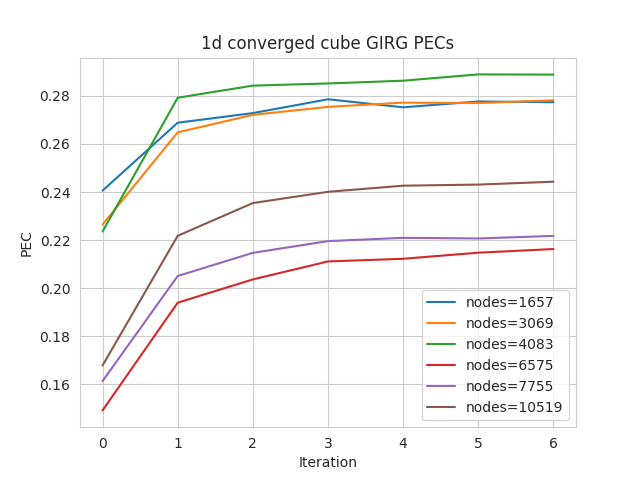
\includegraphics[width=0.49\textwidth]{figures/mcmc_ordered_1d_pec_convergence.png}
  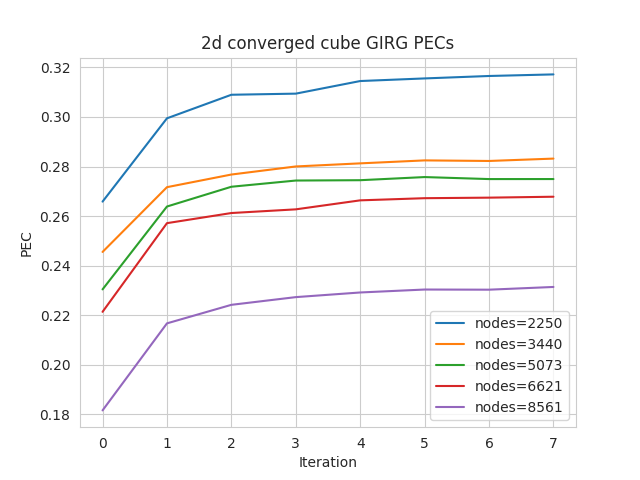
\includegraphics[width=0.49\textwidth]{figures/mcmc_ordered_2d_pec_convergence.png}
  \caption{PEC convergence over iterations for some example graphs.}
\end{figure}


\begin{figure}
  \centering
  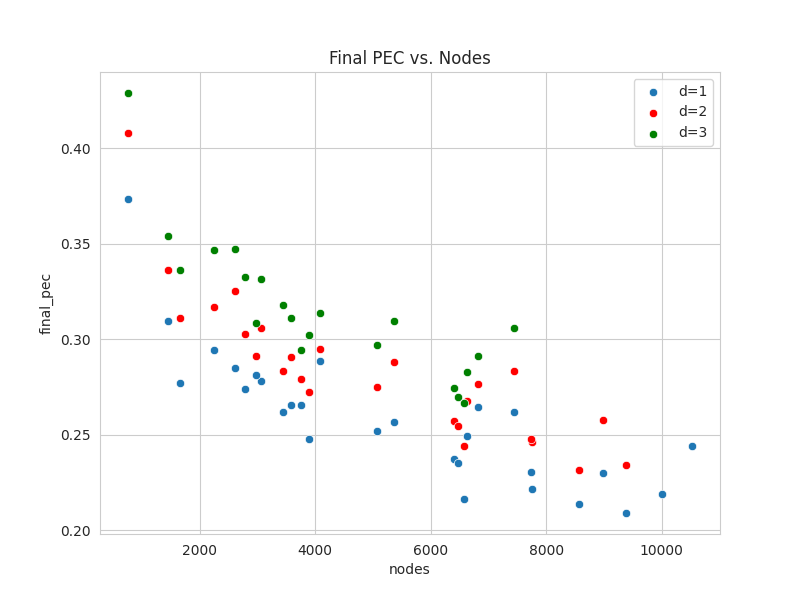
\includegraphics[width=\textwidth]{figures/mcmc_ordered_final_pec.png}
  \caption{converged PECs for 1d, 2d, 3d cube GIRGs. Missing some 3d numbers
  as batch job exceeded allotted time.}
  \label{fig:converged_pecs}
\end{figure}

% \subsection{point initalisation and failure rate}
% Initially I ran MCMC using uniformified diffusion map initialisation, and failure rate $0.0$. The MCMC would converge, but actually take longer than necessary, as the "good" initialisation was being undone in favour of quite spaced out points.

% The evidence for this is shown in some plots of points over time:

% \begin{figure}
%   \centering
%   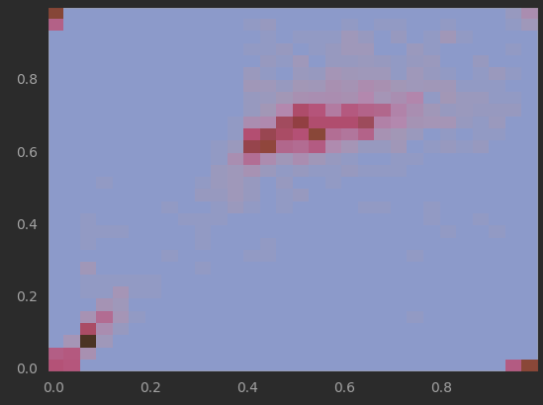
\includegraphics[width=\textwidth]{figures/amherst_2d_pts_restricted.png}
%   \caption{0.05 quantile restricted and uniformed at the edges diffusion map initialisation of MCMC points for socfb-Amherst41}
% \end{figure}

% \begin{figure}

%   \begin{subfigure}{1.0\textwidth}
%   \centering
%   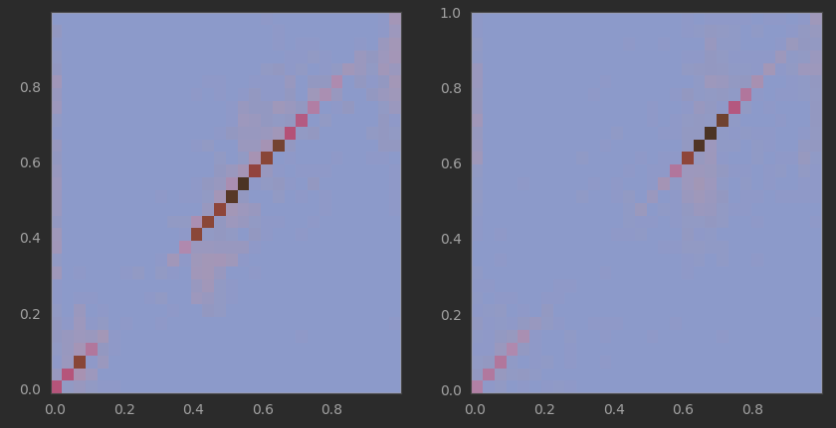
\includegraphics[width=\linewidth]{figures/amherst_failure_mcmc_pts.png}
%   \caption{failure rate $0.3$}
% \end{subfigure}

%   \vspace{1em}

%   \begin{subfigure}{1.0\textwidth}
%   \centering
%   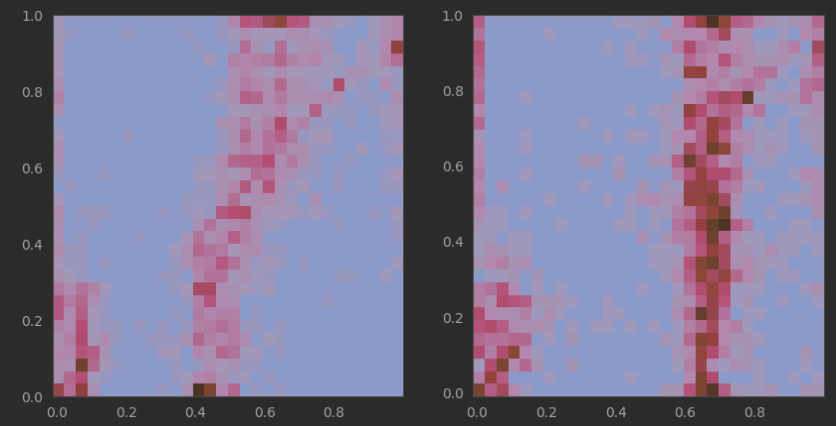
\includegraphics[width=\linewidth]{figures/amherst_nonfailure_mcmc_pts.png}
%   \caption{failure rate $0.0$ (aka no failure rate)}
% \end{subfigure}

%   \caption{MCMC iterated points scatter plot against initialisation, with/without failure rate}
%   \label{fig:amherst_points_over_time}
% \end{figure}


% Run long enough, the MCMC's points converge to the cube:

% \begin{figure}
%   \centering
%   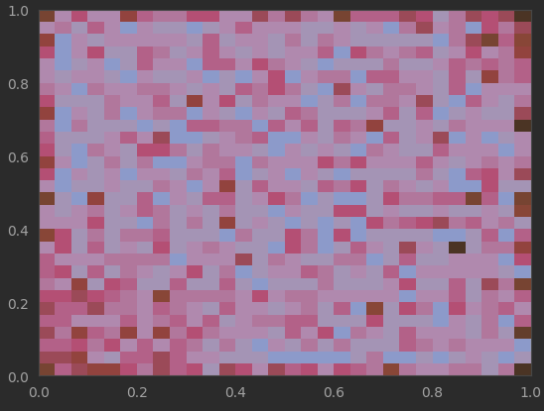
\includegraphics[width=\textwidth]{figures/MCMC_converged_to_cube.png}
%   \caption{failure rate $0.0$ run until convergence for 2D GIRG: points 2D histogram}
% \end{figure}


% \begin{table}[ht]
%   \centering
%   \begin{tabular}{|l|l|}
%   \hline
%   \textbf{LL maximum for 1D} & \textbf{LL maximum for 2D} \\
%   \hline
%   socfb-Amherst41 & socfb-Bowdoin47 \\
%   socfb-Oberlin44 & socfb-Caltech36 \\
%   socfb-Reed98 & socfb-Colgate88 \\
%   socfb-Swarthmore42 & socfb-Hamilton46 \\
%   socfb-Wellesley22 & socfb-Haverford76 \\
%   & socfb-Middlebury45 \\
%   & socfb-Pepperdine86 \\
%   & socfb-Santa74 \\
%   & socfb-Simmons81 \\
%   & socfb-Smith60 \\
%   & socfb-Trinity100 \\
%   & socfb-USFCA72 \\
%   & socfb-Vassar85 \\
%   & socfb-Williams40 \\
%   \hline
%   \end{tabular}
%   \caption{Your Caption}
%   \label{tab:my_label}
%   \end{table}




%   \begin{figure}
%     \centering

%     \begin{subfigure}{0.49\textwidth}
%       \centering
%       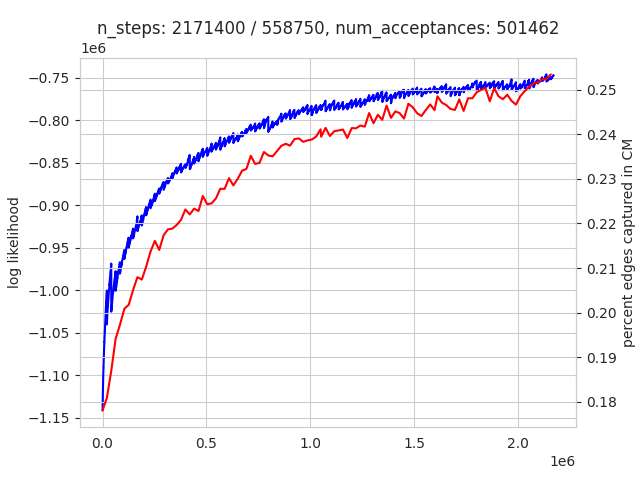
\includegraphics[width=\linewidth]{figures/MCMC_plots/socfb-Amherst41-1d.png}
%       \caption{Amherst41 $d=1$}
%     \end{subfigure}
%     \hfill
%     \begin{subfigure}{0.49\textwidth}
%       \centering
%       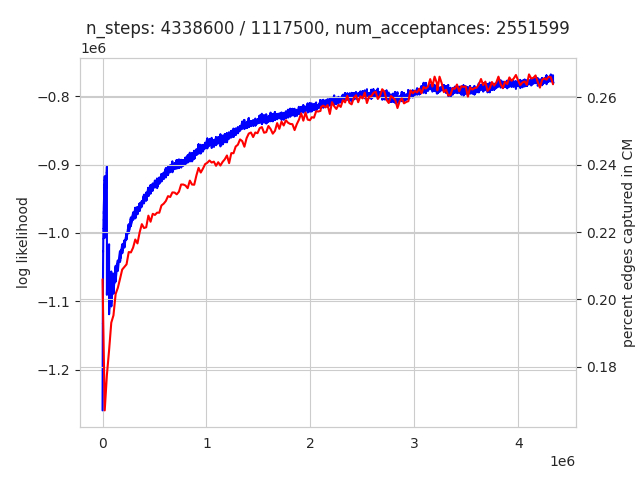
\includegraphics[width=\linewidth]{figures/MCMC_plots/socfb-Amherst41-2d.png}
%       \caption{Amherst41 $d=2$}
%     \end{subfigure}
  
%     \vspace{1em}

%     \begin{subfigure}{0.49\textwidth}
%       \centering
%       \includegraphics[width=\linewidth]{figures/MCMC_plots/socfb-Trinity100-1d.png}
%       \caption{Trinity100 $d=1$}
%     \end{subfigure}
%     \hfill
%     \begin{subfigure}{0.49\textwidth}
%       \centering
%       \includegraphics[width=\linewidth]{figures/MCMC_plots/socfb-Trinity100-2d.png}
%       \caption{Trinity100 $d=2$}
%     \end{subfigure}
  
%     \vspace{1em}
%     \begin{subfigure}{0.49\textwidth}
%       \centering
%       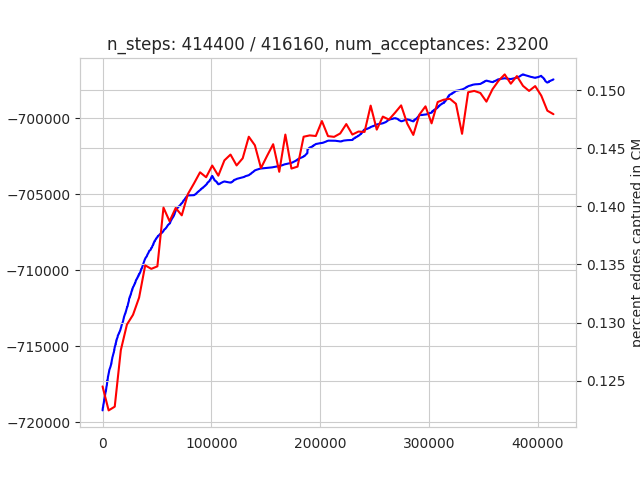
\includegraphics[width=\linewidth]{figures/MCMC_plots/socfb-Hamilton46-1d.png}
%       \caption{Hamilton46 $d=1$}
%     \end{subfigure}
%     \hfill
%     \begin{subfigure}{0.49\textwidth}
%       \centering
%       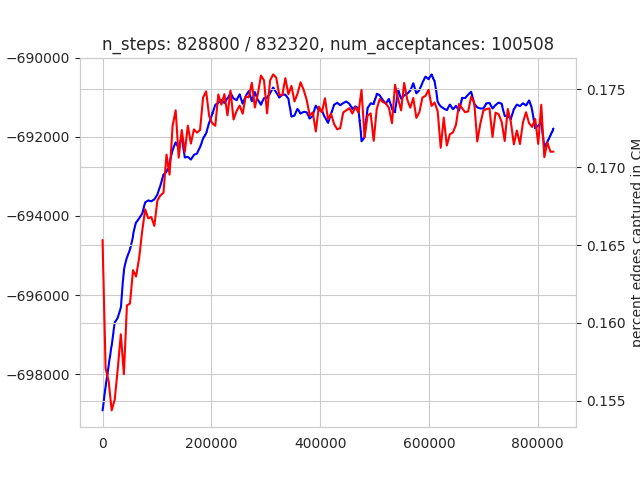
\includegraphics[width=\linewidth]{figures/MCMC_plots/socfb-Hamilton46-2d.png}
%       \caption{Hamilton46 $d=2$}
%     \end{subfigure}
  
%     % \vspace{1em}
%     % \begin{subfigure}{0.49\textwidth}
%     %   \centering
%     %   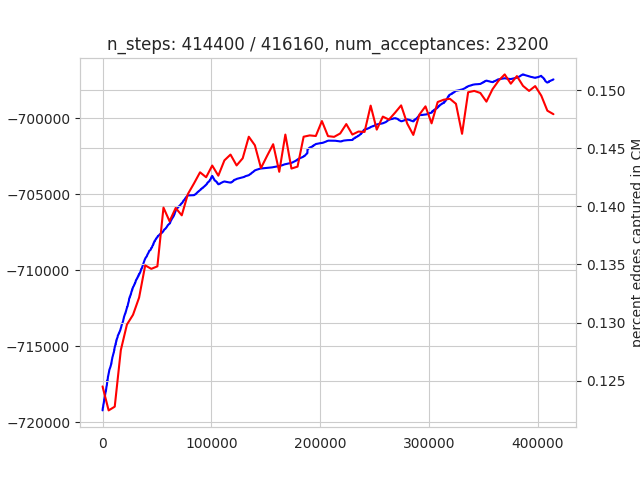
\includegraphics[width=\linewidth]{figures/MCMC_plots/socfb-Hamilton46-1d.png}
%     %   \caption{$d=1$}
%     % \end{subfigure}
%     % \hfill
%     % \begin{subfigure}{0.49\textwidth}
%     %   \centering
%     %   \includegraphics[width=\linewidth]{figures/MCMC_plots/socfb-Hamilton46-2d.png}
%     %   \caption{$d=2$}
%     % \end{subfigure}
  
%     % \vspace{1em}
%     % \begin{subfigure}{0.49\textwidth}
%     %   \centering
%     %   \includegraphics[width=\linewidth]{figures/MCMC_plots/socfb-Hamilton46-3d.png}
%     %   \caption{$d=1$}
%     % \end{subfigure}
%     % \hfill
%     % \begin{subfigure}{0.49\textwidth}
%     %   \centering
%     %   \includegraphics[width=\linewidth]{figures/MCMC_plots/socfb-Reed98-1d.png}
%     %   \caption{$d=2$}
%     % \end{subfigure}
  
%     % \vspace{1em}

  
%     \caption{MCMC runs for socfb-Amherst41, sofcb-Trinity100, socfb-Hamilton46 with failure rate $0.3$ and ChungLu Mixin rate $0.5$ Log likelihood wise, Amherst 1D GIRG does best; for Bowdoin it's 2D GIRG}
%     \label{fig:amherst_non_failure_mcmc}
% \end{figure}


\appendix

\chapter{Appendix}
\minitoc
You can defer lengthy calculations that would otherwise only interrupt
the flow of your thesis to an appendix.


\section{Graph Kernels}
\label{chap:graph_kernels}

In this section we try to compare the bayesian evidence based plausibility of different GGMs in generating Facebook graphs by using the method of \textit{graph kernels}. Unfortunately the whole endeavour was unsuccessful, but we nonetheless briefly detail the framework and our experiments.

\subsection{Bayes Factor Theory}
A bayesian approach to model selection is to compare the posterior probability of different models $p(M_1 | D)$ vs $p(M_2 | D)$, given the model generative processes $P(D | M)$. 
$M_1, M_2$ are possible models of the data, e.g. $M_1 = \cG_{1D\; \GIRG}$ and $M_2 = \cG_{CL}$.
$D$ is a single graph instance $G$, or alternatively a whole dataset of our 100 Facebook graphs, assuming that they all come from the same generative model family.
We have some prior of $p(M_1)$ vs $p(M_2)$, e.g. $50 : 50$. We could even possibly have a set of models $M_{d=1}, M_{d=2}, M_{d=3}, ...$ for different dimensional GIRGs with some kind of decaying $p(1d\; \GIRG) > p(2d\; \GIRG) > p(3d\; \GIRG) > \dots$.

For now focussing on just $M_1$ vs $M_2$,
\begin{equation}
  p(M_1 | D) = \frac{p(D | M_1) p(M_1)}{p(D)} 
  \;
  \implies
  \;
  \frac{p(M_1 | D)}{p(M_2 | D)} = \frac{p(D | M_1) p(M_1)}{p(D | M_2) p(M_2)}
\end{equation}
Model selection is done with the ratio $\frac{p(M_1 | D)}{p(M_2 | D)}$ which is called the \textit{Bayes Factor}.
In order to compute the bayes factor, we will for now ignore the priors $p(M_1), p(M_2)$, and hence focus just on the likelihoods $p(D | M_1), p(D | M_2)$.



\subsubsection{Graph isomorphism problem in computing model evidence}
In our case if $M_1$ is a 1D GIRG, and we've decided to fix 
% $\alpha, e, \{w_u\}_{u \in V}$
$\alpha, \{w_u\}_{u \in V}$
 and just vary $\theta = c, \{\vec{x}_u\}_{u \in V}$, then we could Monte Carlo sample $\theta \sim p(\theta)$ from the prior to get an estimate for
\begin{equation} \label{eq:incorrect_girg_model_likelihood}
  p(D| M_1) = p(G | \cG_{\text{1d-}\GIRG}) = \int_\theta p(G | \theta, \cG_{\text{d-}\GIRG}) p(\theta | \cG_{\text{d-}\GIRG}) d\theta
\end{equation}
% $p(D | M_1) = p(G) = \int_\theta p(G | \theta) p(\theta) d\theta$, 
The simplified notation is dropping the $| M_1$ as we fix into some dimensional GIRG universe, $\int_\theta p(G | \theta) p(\theta) d\theta$.

There's a problem here. Since our data is a graph $D=G$, in the computation we actually need to inspect $p(G | \theta) = \sum_{\sigma} p(G' \stackrel{\sigma}{\cong} G | \theta) p(\sigma)$. Here $\sigma$ is a permutation of the node ID, and $\stackrel{\sigma}{\cong}$ denotes \textit{graph isomorphism} under this permutation. Note here our abuse of notation - normally $p(G | \theta)$ is not a sum over permutations, but rather the probability of generating this exact graph $G$; this will have to be contextually apparent. So instead of evaluating $p(G | \theta)$, we rather want to evalute \q{the probability of producing $G'$, given parameters $\theta$, which is isomorphic to $G$}.

% Hence our simple Monte Carlo computation of $p(G | \theta, \GIRG) < p(G | CL)$ which was sad, is actually not quite valid. So Yay! We can still hope that the GIRG model is better than Chung-Lu, or at least bayesianly more likely.

% To be concrete, \cref{fig:automorphic_isomorphic_graphs} shows an example of graph auto/isomorphisms with different permutations $\sigma$.
% % As a concrete example, let's say $G=(1,2), (2, 3), (2, 4), (2, 5)$. Then we say $G$ is isomorphic to $G'$ with permutation $\sigma= (1,4)$ ($G \stackrel{\sigma}{\to} G'$) where $G' = (4, 2), (2, 3), (2, 1), (2, 5)$.
% So the bayesian evidence compuation is actually to sample $\theta$,  then for each $\sigma \in S_n$ create $G'$ where $G$ is isomorphic to $G'$ with permutation $sigma$ ($G \stackrel{\sigma}{\to} G'$), and calculate $p(G' | \theta)$; add these up and take the average.
% Finally repeat for further $\theta$ samples and take an outer average.


% \begin{tikzpicture}
%     \node[circle, draw] (1) at (0, 0) {1};
%     \node[circle, draw] (2) at (2, 0) {2};
%     \node[circle, draw] (3) at (1, 1.732) {3};
  
%     \draw[-] (1) -- (2);
  
% \end{tikzpicture}

\begin{figure}
    \begin{tikzpicture}[scale=1.5]
        % Graph 1
        \node[circle, draw] (g1v1) at (0, 0) {2};
        \node[circle, draw] (g1v2) at (1, 0) {1};
        \node[circle, draw] (g1v3) at (0.5, 0.866) {3};
    
        \draw[-] (g1v1) -- (g1v2);
    
        % Graph 2 (Automorphism)
        \node[circle, draw] (g2v2) at (3, 0) {1};
        \node[circle, draw] (g2v1) at (4, 0) {2};
        \node[circle, draw] (g2v3) at (3.5, 0.866) {3};
    
        \draw[-] (g2v2) -- (g2v1);
    
        % Graph 3
        \node[circle, draw] (g3v3) at (6, 0) {3};
        \node[circle, draw] (g3v2) at (7, 0) {2};
        \node[circle, draw] (g3v1) at (6.5, 0.866) {1};
    
        \draw[-] (g3v2) -- (g3v3);

        % % Arrows
        % \draw[->, thick] (g2v2) to[out=135,in=45] node[midway, above] {2 $\rightarrow$ 1} (g1v2);
        % \draw[->, thick] (g2v2) to[out=-135,in=-45] node[midway, below] {2 $\rightarrow$ 3} (g3v2);
      
        % Arrows
        \draw[<-, thick] (1.8, 0.2) -- node[midway, above] {$\sigma = (1\; 2)$} (2.3, 0.2);
        \draw[->, thick] (4.7, 0.2) -- node[midway, above] {$\sigma = (1\; 3)$} (5.2, 0.2);

    
        % Labels
        \node[align=center] at (0.5, -0.7) {$G_2$ \\Automorphic to $G_1$};
        \node[align=center] at (3.5, -0.7) {$G_1$};
        \node[align=center] at (6.5, -0.7) {$G_3$\\ Isomorphic to $G_1, G_2$};
    
    \end{tikzpicture}
    \caption{Example automorphic/isomorphic graphs}
    \label{fig:automorphic_isomorphic_graphs}
\end{figure}

\paragraph{Small concrete example} of a labelled graph $G_1 = (V, E) = (\{1, 2, 3\}, \{(1,2)\})$ which is shown in \cref{fig:automorphic_isomorphic_graphs}. $G_1$ is isomorphic to any other labelled graph $H$ if they look the same if you anonymise the nodes.
More formally, if $\sigma: V(G) \to V(H)$ is a bijection mapping nodes to nodes, such that $u \sim v$ in $G$ $\iff \sigma(u) \sim \sigma(v)$ in $H$, then $G$ is isomorphic to $H$ with permutation $\sigma$, written $G \stackrel{\sigma}{\cong} H$.
So $G_1$ is isomorphic to $G_3$ with edge set $\{(3,2)\}$. You can even say that it is automorphic to the graph $H$ with edge set $\{(2, 1)\}$, i.e. just switching nodes $1,2$.
On this graph $G_1$ of 3 nodes, there are $3! = 6$ node ID permutations, each of which produces an isomorphic graph $G'$. For our particular $G_1$, we could group together these 6 isomorphic graphs $G'$ into 3 pairs of automorphic graphs.

% Hence the bayesian evidence compuation is actually to sample $\theta$,  then for each $\sigma \in S_n$ create $G'$ where $G$ is isomorphic to $G'$ with permutation $sigma$ ($G \stackrel{\sigma}{\to} G'$), and calculate $p(G' | \theta)$; add these up and take the average.
Finally repeat for further $\theta$ samples and take an outer average.


Consider a simplified Chung-Lu / GIRG model of three nodes where of $\theta = (\vec{x}_1, \vec{x}_2, \vec{x}_3)$ and all nodes have the same weight $1$.
The Chung-Lu has identical $p(G')$ for each of the 6 ismorphisms.
The GIRG  model does not - if $\vec{x}_1, \vec{x}_2$ are close, and $\vec{x}_3$ is far from both, then it awards higher probability to $G' = (V, \{(1,2)\})$ and $G' = (V, \{(2, 1)\})$.
Furthermore both models always award the same probability to any equivalent class of automorphic graphs - this is because the adjacency matrix is the same for automorphic graphs, which is all that the models care about.

Unfortunately computing the $n!$ length sum $\sum_{\sigma} p(G' \stackrel{\sigma}{\cong} G | \theta) p(\sigma)$ is infeasible for all but tiny graphs. As an alternative, we hoped to use a graph similarity kernel $k$ which compares two graphs $G, H$, giving some measure $k(G, H)$ of how similar they are up to ismorphism (in a node permutation invariant way).
% Apparently one more computable example is the random walk kernel.
Therefore the idea would be to replace the
\begin{align}
  \text{replace the incorrect} \quad p(G | \cG_\GIRG) = \int_\theta p(G | \theta) p(\theta) d\theta
  \\
  \text{with} \quad
% $\mu(G) = \int_\theta k(G, G' \sim \cG_\theta) p(\theta) d\theta$. This is an idea.
E_{G' \sim \cG_{\GIRG}} \left [ k(G, G') \right ]\approxeq \frac{1}{m} \sum_{i=1}^m k(G, G'_i \sim \cG_\GIRG)
\end{align}
which is Monte Carlo computable.
% Therefore the idea would be to replace the incorrect $p(G | \cG_{\text{d-}\GIRG}) = \int_\theta p(G | \theta, \cG_{\text{d-}\GIRG}) p(\theta | \cG_{\text{d-}\GIRG}) d\theta$ with $\mu(G) = E_{G' \sim \cG_{\text{d-}\GIRG}} \left [ k(G, G') \right ]$. This is an idea.

% So when we say $p(G | \theta)$, we actually mean the probability of getting a graph $G'$ which is isomorphic to $G$, given parameters $\theta$.



% TODO do we remove this weird figure - what's it doing here? 
% \begin{figure}
%     \centering

%     \begin{subfigure}{0.49\textwidth}
%       \centering
%       \includegraphics[width=\linewidth]{figures/socfb-Amherst41-1d.png}
%       \caption{$d=1$}
%     \end{subfigure}
%     \hfill
%     \begin{subfigure}{0.49\textwidth}
%       \centering
%       \includegraphics[width=\linewidth]{figures/socfb-Amherst41-2d.png}
%       \caption{$d=2$}
%     \end{subfigure}
  
%     \vspace{1em}
  
%     \begin{subfigure}{0.49\textwidth}
%       \centering
%       \includegraphics[width=\linewidth]{figures/socfb-Amherst41-3d.png}
%       \caption{$d=3$}
%     \end{subfigure}
%     \hfill
  
%     \caption{MCMC runs for socfb-Amherst41, without failure rate}
%     \label{fig:amherst_non_failure_mcmc}
% \end{figure}

% We see in \cref{fig:amherst_non_failure_mcmc} that Bayes Factor model comparison wise, 1D GIRGs are superior, even though according to edge accuracy, 2D GIRGs achieve a slight edge.


\subsection{Graph Kernel Introduction}
Graph Kernels provide a means for a similarity metric between graphs. They're ideally a positive semidefinite function $k: \Gamma \times \Gamma \rightarrow \mathbb{R}$, where $\Gamma$ is the set of all graphs. Such a function exists if and only if there is a corresponding feature map resentation of $\phi: \Gamma \to \cH_\phi$ where $\cH_\phi$ is a Hilbert space, and $k(G, G') = \langle \phi(G), \phi(G') \rangle_{\cH_\phi}$ is just an inner product.

Graph kernels can be contrasted with the Blasius' GGM realism framework . Blasius compares multiple different graph feature combinations on which to train an SVM for distinguishing two graph datasets.
Viewing the graph kernel as an inner product of graph feature maps, these hopefully encapsulate all the relevant information about the graph including the specifically chosen features in Blasius' framework like graph diameter, average degree, etc. The question of which chosen graph features to consider then shifts to which graph kernel to use!

% Instead we can replace this with a single kernel which hopefully encapsulates sufficient relevant information about the graphs - viewed as an inner product between graph . The question of which graph features to use then shifts to which graph kernel to use!

% Another benefit of graph kernels is, as a similarity metric, they give easier direct comparison between graphs.
% In the previous sections' proposed paradigm, we can directly compare the similarity of a real graph $G$ with two synthetic graphs $G_1, G_2$, produced from different models $M_1, M_2$, using $k(G, G_1)$ and $k(G, G_2)$.
% This is simply done by comparing $k(G, G_1)$ and $k(G, G_2)$ - the higher of the two is the more similar.


% Graph Kernels have many uses, but we can use them in particular to help with bayesian model comparison, solving our issue of graph permutations.

% A survey on graph kernels https://appliednetsci.springeropen.com/articles/10.1007/s41109-019-0195-3



% We saw the equation $\mu(G) = E_{G' \sim \cG_{\text{d-}\GIRG}} \left [ k(G, G') \right ]$ in the previous chapter. We can Monte Carlo sample this expectation to get an estimate.


There are a range of graph kernels to choose from, however given the relatively large size of our graphs, runtime can be an issue. We ended up testing two kernels; alas both proved unsatisfactory. Without further expertise on graph kernels, we were forced to abandon this line of attack. We think that graph kernels might be more effective on smaller graphs with more unique structure (our random graph models and the real graphs themselves have a lot of homogenous structure) and particularly graphs with meangingful node labels.

\subsubsection{Random walk kernel}
The \textit{random walk kernel} between two graphs is just a count of the number of common walks in the pair,  of any length $l$. Thißs is generally an infinite sum, so geometric weighting with the factor $\lambda^l$ is used to decay the contribution of longer walks, where $0 < \lambda < 1$ (we tested with $\lambda=10^{-5}$).

The product graph of $G$ and  $G'$ is defined as 
\begin{align}
  G_\times = (V_\times, E_\times) \quad \text{where} \quad V_\times = \{(v, v') | v \in V, v' \in V'\}\\
  \text{and} \quad E_\times = \{((v_1, v'_1), (v_2, v'_2)) | v_1 \sim v_2 \in E_1, v'_1 \sim v'_2 \in E_2\}
\end{align}
This definition can be extended to node-labelled graphs, where we only take product vertices $(v, v') \in V_\times$ if $v \in V, v' \in V'$ have the same label. Common walks in the pair of graphs $G,G'$ are just walks in the product graph.

The naive implementation of the random walk kernel has complexity $O(n^6)$, however this can be sped up to $O(n^3)$. This is still too slow for our purposes. We only made limited tests with small graphs of $n \leq 3000$ nodes - see e.g. \cref{fig:rw_kernel_fitcopycube}.

\subsubsection{Weisfeiler-Lehman kernel}
The \textit{Weisfeiler-Lehman kernel} runs much faster in $O(h|E|)$ time, where $|E|$ is the number of edges in the graph and $h$ is a chosen parameter, the number of rounds of relabelling within the algorithm. The algorithm requires some starting node labels $(l(v))_{v \in V}$ - we colour nodes into a small discreet set of colours by grouping together nodes with similar sized degrees. It also uses a base kernel $k_{\text{base}}$ which is computed at each relabelling round  - we used the simplest/speediest node label \textit{histogram dot product kernel}:
\begin{equation}
  k(G, G') = \langle \vec{f}, \vec{f}' \rangle \quad \text{where} \quad \vec{f} = (f_1, \dots, f_k), \;f_i = |\{ v \in V \;:\; l(v) = i\}|
\end{equation}
The Weisfeiler-Lehman kernel is then defined as
\begin{align}
  k_{WLK}(G, G') = k_{\text{base}}(G_1, G_1') + \dots + k_{\text{base}}(G_h, G_h')
\\
G =G_1,\; G' = G'_1 ; \quad G_{i+1}\; \text{by relabelling} \; G_i: \quad l(v) \gets (l(v), (l(u))_{u \sim v})
\end{align}
% $G=G_1,\; G' = G'_1$, and $G_{i+1}$ is computed iteratively as relabelling each node in $G_i$ with $l(v) \gets (l(v), (l(u))_{u \sim v})$.
This looks odd, but in practice each label is just rehashed as a new integer rather than becoming a highly nested tuple.



\subsection{Experiments}

Unfortunately both kernels failed to pass the basic test of showing higher similarity between two graphs generated from the same GGM than from a different GGM. We tried a variety of combinations, but didn't get very reliable results: see \cref{fig:wl_kernel_gentorus} and \cref{fig:rw_kernel_fitcopycube}.

% E.g. in \cref{fig:rw_kernel_fitcopycube}, the random walk kernel faield the basic test of having $k(G \sim \cG_1, G'_1 \sim \cG_1) > k(G \sim \cG_1, G'_2 \sim \cG_2)$, where $\cG_1$ is a 3D copy weight cube GIRG, and $\cG_2$ is copy weight Chung-Lu.

\begin{figure}
  \centering

  \begin{subfigure}{0.49 \textwidth}
    \centering
    \includegraphics[width=\linewidth]{figures/d=2 alpha=1.2 n=70000 GIRG WL-Kernel with others.png}
    \caption{Weisfeiler-Lehman Kernel of a d=2, alpha=1.2, n=70000 Torus GIRG with other generated graphs (13 per model). All the GIRGs are more similar to the original than Chung-Lu, which is good, but we cannot differentiate between GIRGs of different dimensions.}
    \label{fig:wl_kernel_gentorus}
  \end{subfigure}
  \hfill
  \begin{subfigure}{0.49 \textwidth}
    \centering
    \includegraphics[width=\linewidth]{figures/socfb-Brandeis99 d=3.png}
    \caption{Random Walk Kernel of a d=3 copy weight cube GIRG fit to socfb-Brandeis99 (matching number of edges and mean LCC), with other graphs generated from different GGMs (6 per model type). We hoped for 3d GIRGs to have the highest similarity to the input graph, however instead Chung-Lu graphs matched closest.}
    \label{fig:rw_kernel_fitcopycube}
  \end{subfigure}
\end{figure}


% \begin{figure}
%   \centering
% \includegraphics[width=0.8\linewidth]{figures/d=2 alpha=1.2 n=70000 GIRG WL-Kernel with others.png}
% \caption{WL-Kernel of a d=2, alpha=1.2, n=70000 Torus GIRG with other generated graphs (13 per model). All the GIRGs are more similar to the original than Chung-Lu, but we cannot differentiate between GIRGs of different dimensions.}
% \label{fig:wl_kernel_gentorus}
% \end{figure}

% % socfb-Brandeis99 d=3.png


% \begin{figure}
%   \centering
% \includegraphics[width=0.8\linewidth]{figures/socfb-Brandeis99 d=3.png}
% \caption{RW-Kernel of a d=3 copy weight cube GIRG fit to socfb-Brandeis99 (matching number of edges and local clustering coefficient), with other generated graphs (6 per model type). Chung-Lu graphs have highest similarity to the original, despite it being a 3D GIRG}
% \label{fig:rw_kernel_fitcopycube}
% \end{figure}



% We think that 


% \subsection{Experiments}
% we do the comparison

% Cube Similarity Plots:
% We fit alpha, c for a uniform cube GIRG for dimensions d=1-3, produce a graph, and look at similarity with real graph.


\backmatter

\bibliographystyle{apalike}
\bibliography{refs}

\includepdf[pages={-}]{declaration-originality.pdf}

\end{document}
